\documentclass[a4paper,11pt,twoside]{report}


% -------------- Kodowanie znaków, język polski -------------

\usepackage[utf8]{inputenc}
\usepackage[MeX]{polski}
%\usepackage[T1]{fontenc}
\usepackage[english, polish]{babel}


% ----------------- Przydatne pakiety ----------------------
\usepackage{amsfonts}
\usepackage{mathrsfs} 
\usepackage{amsmath,amsthm,latexsym,xpatch}
\usepackage[dvips]{graphicx,color}
\usepackage{enumerate}
\usepackage{enumitem}
\usepackage{verbatim}
\usepackage{array}
\usepackage{pstricks}
\usepackage{textcomp}
\usepackage{listings}
\usepackage{xcolor}
\usepackage[none]{hyphenat}
\usepackage{float}
\usepackage{flafter}
\usepackage{pdfpages}
\usepackage{subcaption}
\usepackage{caption} \captionsetup[table]{singlelinecheck=false}		
\usepackage{listings,xcolor}

% ---------------- Marginesy, akapity, interlinia ------------------

\usepackage[inner=20mm, outer=20mm, bindingoffset=10mm, top=25mm, bottom=25mm]{geometry}


\linespread{1.15}
%\allowdisplaybreaks
\usepackage{indentfirst} % opcjonalnie; pierwszy akapit z wcięciem
\setlength{\parindent}{5mm}

\hyphenation{Syl-ves-tra}
\hyphenation{Syl-ves-ter-a}

%--------------------------- ŻYWA PAGINA ------------------------

\usepackage{fancyhdr}
\pagestyle{fancy}
\fancyhf{}
% numery stron: lewa do lewego, prawa do prawego 
\fancyfoot[LE,RO]{\thepage} 
% prawa pagina: zawartość \rightmark do lewego, wewnętrznego (marginesu) 
\fancyhead[LO]{\sc \nouppercase{\rightmark}}
% lewa pagina: zawartość \leftmark do prawego, wewnętrznego (marginesu) 
\fancyhead[RE]{\sc \leftmark}

\renewcommand{\chaptermark}[1]{
\markboth{\thechapter.\ #1}{}}

% kreski oddzielające paginy (górną i dolną):
\renewcommand{\headrulewidth}{0 pt} % 0 - nie ma, 0.5 - jest linia


\fancypagestyle{plain}{% to definiuje wygląd pierwszej strony nowego rozdziału - obecnie tylko numeracja
  \fancyhf{}%
  \fancyfoot[LE,RO]{\thepage}%
  
  \renewcommand{\headrulewidth}{0pt}% Line at the header invisible
  \renewcommand{\footrulewidth}{0.0pt}
}



% ---------------- Nagłówki rozdziałów ---------------------

\usepackage{titlesec}
\titleformat{\chapter}%[display]
  {\normalfont\Large \bfseries}
  {\thechapter.}{1ex}{\Large}

\titleformat{\section}
  {\normalfont\large\bfseries}
  {\thesection.}{1ex}{}
\titlespacing{\section}{0pt}{30pt}{20pt} 
%\titlespacing{\co}{akapit}{ile przed}{ile po} 
    
\titleformat{\subsection}
  {\normalfont \bfseries}
  {\thesubsection.}{1ex}{}


% ----------------------- Spis treści ---------------------------
\def\cleardoublepage{\clearpage\if@twoside
\ifodd\c@page\else\hbox{}\thispagestyle{empty}\newpage
\if@twocolumn\hbox{}\newpage\fi\fi\fi}


% kropki dla chapterów
\usepackage{etoolbox}
\makeatletter
\patchcmd{\l@chapter}
  {\hfil}
  {\leaders\hbox{\normalfont$\m@th\mkern \@dotsep mu\hbox{.}\mkern \@dotsep mu$}\hfill}
  {}{}
\makeatother

\usepackage{titletoc}
\makeatletter
\titlecontents{chapter}% <section-type>
  [0pt]% <left>
  {}% <above-code>
  {\bfseries \thecontentslabel.\quad}% <numbered-entry-format>
  {\bfseries}% <numberless-entry-format>
  {\bfseries\leaders\hbox{\normalfont$\m@th\mkern \@dotsep mu\hbox{.}\mkern \@dotsep mu$}\hfill\contentspage}% <filler-page-format>

\titlecontents{section}
  [1em]
  {}
  {\thecontentslabel.\quad}
  {}
  {\leaders\hbox{\normalfont$\m@th\mkern \@dotsep mu\hbox{.}\mkern \@dotsep mu$}\hfill\contentspage}

\titlecontents{subsection}
  [2em]
  {}
  {\thecontentslabel.\quad}
  {}
  {\leaders\hbox{\normalfont$\m@th\mkern \@dotsep mu\hbox{.}\mkern \@dotsep mu$}\hfill\contentspage}
\makeatother



% ---------------------- Spisy tabel i obrazków ----------------------

\renewcommand*{\thetable}{\arabic{chapter}.\arabic{table}}
\renewcommand*{\thefigure}{\arabic{chapter}.\arabic{figure}}
%\let\c@table\c@figure % jeśli włączone, numeruje tabele i obrazki razem


% --------------------- Definicje, twierdzenia etc. ---------------


\makeatletter
\newtheoremstyle{definition}%    % Name
{3ex}%                          % Space above
{3ex}%                          % Space below
{\upshape}%                      % Body font
{}%                              % Indent amount
{\bfseries}%                     % Theorem head font
{.}%                             % Punctuation after theorem head
{.5em}%                            % Space after theorem head, ' ', or \newline
{\thmname{#1}\thmnumber{ #2}\thmnote{ (#3)}}%  % Theorem head spec (can be left empty, meaning `normal')
\makeatother

% ----------------------------- POLSKI --------------------------------
\theoremstyle{definition}
\newtheorem{theorem}{Twierdzenie}[chapter]
\newtheorem{lemma}[theorem]{Lemat}
\newtheorem{example}[theorem]{Przykład}
\newtheorem{proposition}[theorem]{Stwierdzenie}
\newtheorem{corollary}[theorem]{Wniosek}
\newtheorem{definition}[theorem]{Definicja}
\newtheorem{remark}[theorem]{Uwaga}

% If in English, comment this and uncomment below:

% ----------------------------- ENGLISH -----------------------------
%\theoremstyle{definition}
%\newtheorem{theorem}{Theorem}[chapter]
%\newtheorem{lemma}[theorem]{Lemma}
%\newtheorem{example}[theorem]{Example}
%\newtheorem{proposition}[theorem]{Proposition}
%\newtheorem{corollary}[theorem]{Corollary}
%\newtheorem{definition}[theorem]{Definition}
%\newtheorem{remark}[theorem]{Remark}



% ----------------------------- Dowód -----------------------------

\makeatletter
\renewenvironment{proof}[1][\proofname]
{\par
  \vspace{-12pt}% remove the space after the theorem
  \pushQED{\qed}%
  \normalfont
  \topsep0pt \partopsep0pt % no space before
  \trivlist
  \item[\hskip\labelsep
        \sc
    #1\@addpunct{:}]\ignorespaces
}
{%
  \popQED\endtrivlist\@endpefalse
  \addvspace{20pt} % some space after
}

\renewcommand{\qedhere}{\hfill \qedsymbol}
\makeatother





% -------------------------- POCZĄTEK --------------------------


% --------------------- Ustawienia użytkownika ------------------

\newcommand{\tytul}{Implementacja aplikacji wspomagającej diagnostykę nowotworu prostaty, wykorzystującej standard DICOM do integracji z realnym systemem szpitalnym}
\renewcommand{\title}{Implementation of Prostate Cancer (PCa) Computer Aided Diagnosis (CAD) system using DICOM standard for integration in the hospital information system environment.}
\renewcommand{\author}{Łukasz Berwid, Rafał Buzun,  Jakub Karolak}
\newcommand{\album}{268740, 268744, 268758}
\newcommand{\type}{inżyniers} % magisters, licencjac (Master or Engineer in English)
\newcommand{\supervisor}{mgr. inż. Piotr Sobecki}

\lstdefinestyle{sharpc}{language=[Sharp]C, rulecolor=\color{blue!80!black}}


\begin{document}
\sloppy

% \selectlanguage{english} % uncomment this for English 

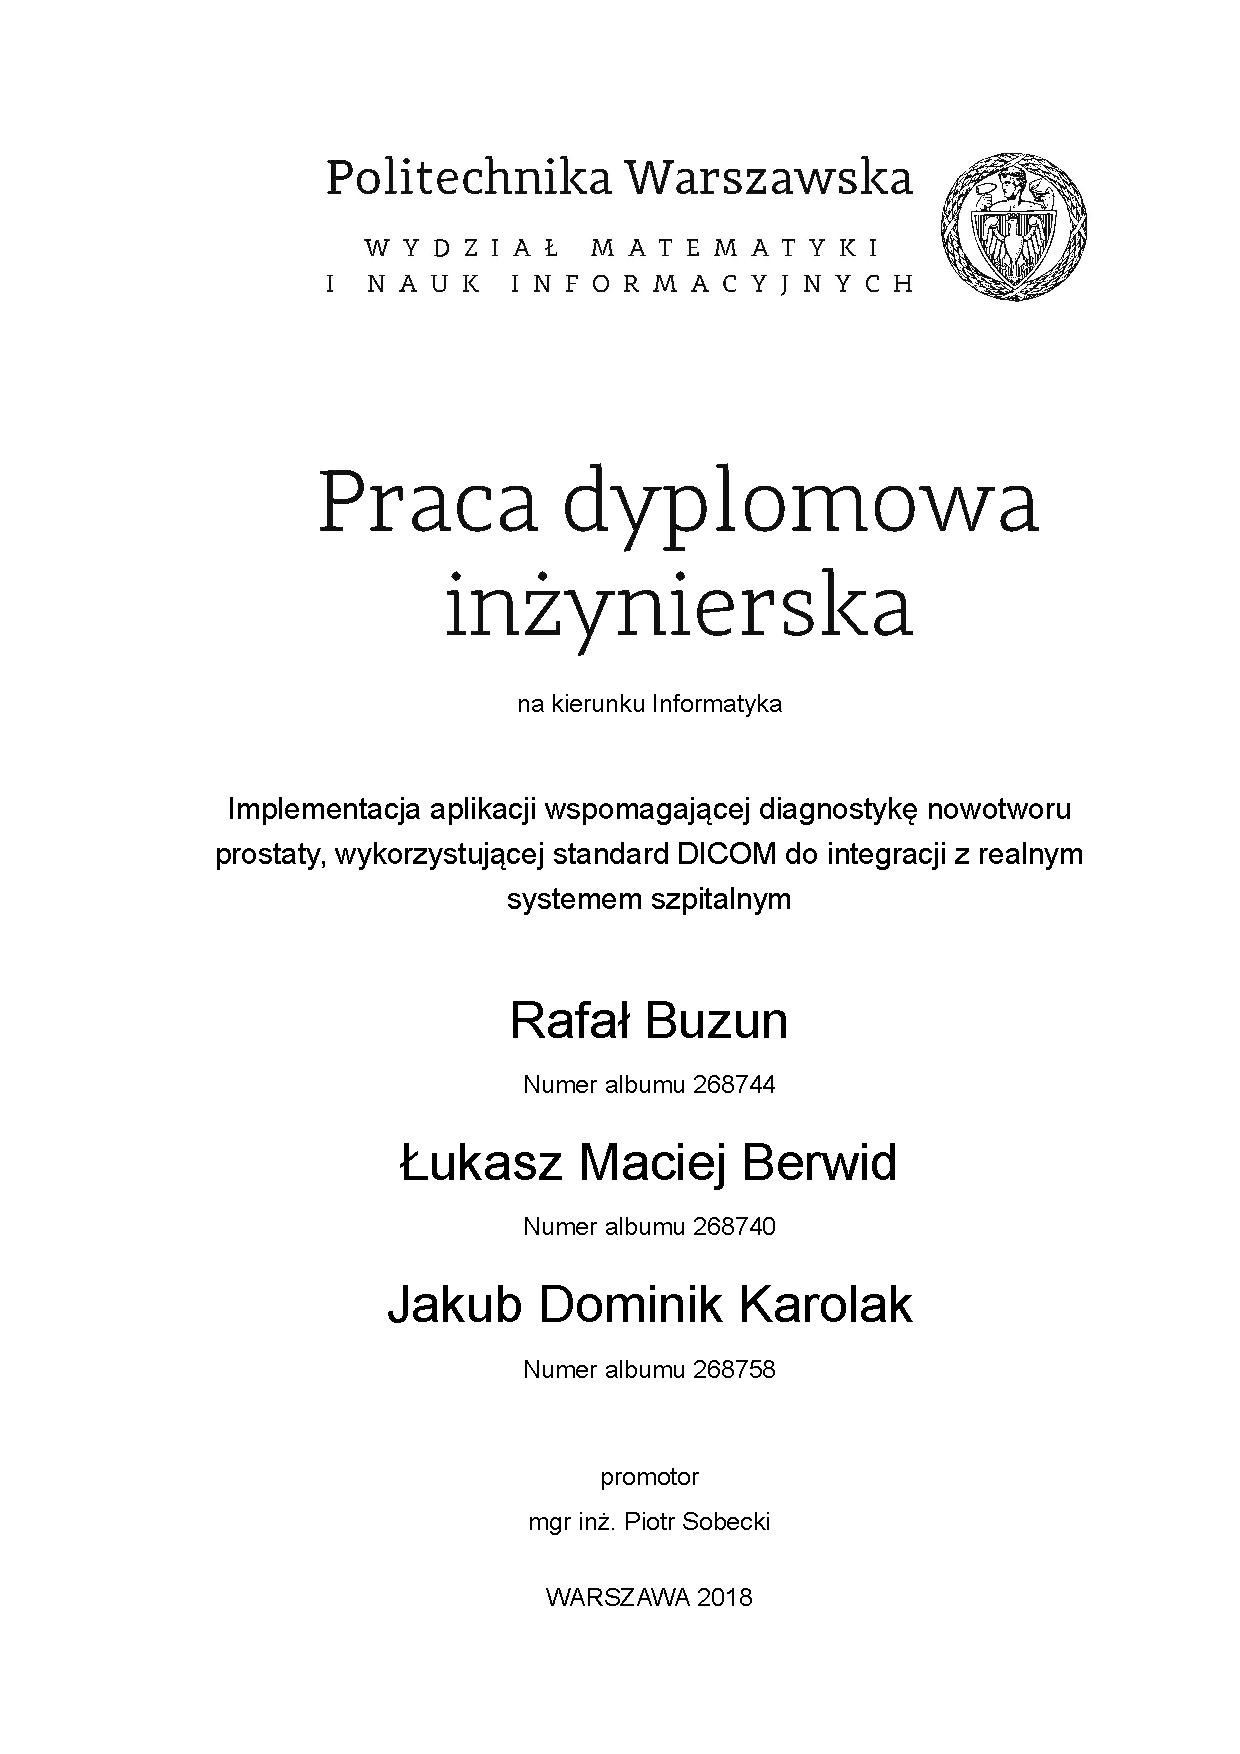
\includepdf[pages=-]{strona-tytulowa-kilku-autorow.pdf}


% ----------------------- Abstrakty -----------------------------

%\selectlanguage{polish}
\begin{abstract}

\begin{center}
\tytul
\end{center}

Celem pracy dyplomowej jest stworzenie narzędzia wspomagającego diagnostykę nowotworu prostaty oraz jego integracja ze szpitalną bazą danych. Proponowane narzędzie będzie umożliwiało obliczanie objętości prostaty bazując na wysegmentowanym fragmencie obrazu pochodzącego z obrazowania metodą multiparametrycznego Rezonansu Magnetycznego. Dodatkowo stworzona zostanie baza badań zawierająca informacje o referencyjnych wartościach objętości gruczołu krokowego pochodzących z estymacji bazującej na obrazowaniu Ultrasonografem. Narzędzie zostanie przygotowane do wdrożenia w szpitalnym systemie informatycznym.

\noindent \textbf{Słowa kluczowe:} przetwarzanie obrazu, analiza danych, bioinformatyka
\end{abstract}

\null\thispagestyle{empty}\newpage

{\selectlanguage{english}
\begin{abstract}

\begin{center}
%\title
\end{center}

The aim of the diploma thesis is to create a tool that supports the diagnostics of prostate cancer and its integration with the hospital database. The proposed tool will be able to calculate prostate volume based on the segmented image from multiparameter Magnetic Resonance imaging. In addition, a database containing information on reference prostate volume values from the estimation based on ultrasonography imaging will be created. The tool will be prepared for implementation in the hospital IT system.

\noindent \textbf{Keywords:} image processing, data analysis, bioinformatics
\end{abstract}}

\null\thispagestyle{empty}\newpage

\null \hfill Warszawa, dnia ..................\\

\par\vspace{5cm}

\begin{center}
Oświadczenie % Declaration - for English
\end{center}

\indent Oświadczam, że moją część pracy \type kiej (zgodnie z podziałem zadań opisanym w~pkt. ...) pod tytułem; ,,\tytul '', której promotorem jest \supervisor \ wykonałem samodzielnie, co poświadczam własnoręcznym podpisem.
\vspace{2cm}


\begin{flushright}
  \begin{minipage}{50mm}
    \begin{center}
      ..............................................

    \end{center}
  \end{minipage}
\end{flushright}

\thispagestyle{empty}
\newpage

\null\thispagestyle{empty}\newpage
% ------------------- 4. Spis treści ---------------------
% \selectlanguage{english} - for English

\thispagestyle{empty}
\tableofcontents
\thispagestyle{empty}
\newpage
% -------------- 5. ZASADNICZA CZĘŚĆ PRACY --------------------
\setcounter{page}{11}
\pagestyle{fancy}

% -------------------- Wstęp -----------------------
\chapter{Wstęp} % Intruduction

Rak prostaty to drugi – zaraz po raku płuc – najczęściej diagnozowany nowotwór u mężczyzn. W ciągu ostatnich lat w Polsce wzrasta zachorowalności na raka stercza, a także – choć w mniejszym stopniu – umieralność. KRN prognozuje, że w naszym kraju w 2015 r. zostanie wykrytych 14 tys. nowych przypadków raka prostaty, a 5 tys. chorych z wcześniej wykrytą chorobą umrze. W 2012 r., zaledwie trzy lata temu, z powodu tego nowotworu zachorowało 11 tys. mężczyzn, a 4,1 tys. zmarło. Odwrotną tendencję obserwuje się w zachodniej Europie i Stanach Zjednoczonych, gdzie odnotowuje się spadek zachorowalności i umieralności na ten nowotwór. Wszystko dzięki zastosowaniu najnowszych metod leczenia i wczesnej diagnostyce. \cite{rynekZdrowia}
\par
Dlatego też, w niniejszej pracy podjęto się zbadania możliwości automatyzacji wykrywania prostaty na zdjęciach rezonansu magnetycznego., poprzez automatyczną segmentację prostaty i obliczanie objętości. Opisane poniżej algorytmy obliczania wielkości gruczołu mogą być wskazówka dla lekarza podczas stawiania diagnozy. 
\par
System powstały jako produkt poniższej pracy dzięki zastosowaniu modularnej architektury może być dostosowany do zaawansowanych systemów szpitalnych oraz rozszerzony o alternatywne algorytmy na przykład oparte o głębokie uczenie maszynowe.
\par
Za implementację oraz wdrożenie algorytmu segmentacji prostaty bazującej na danych konkursowych przy użyciu konwolucyjnych sieci neuronowych oraz moduł prezentacji aplikacji odpowiada Rafał Buzun.
\par
Za stworzenie, opisanie zbioru testowego, przeprowadzenie analizy biznesowej oraz statystycznej wyników badań rezonansu magnetycznego oraz rozpoznanie architektury szpitalnego systemu informatycznego i integrację z systemem PACS odpowiada Jakub Karolak.
\par
Za zaprojektowanie architektury oraz implementacje serwera, w tym obsługę bazy danych i przetwarzanie plików DICOM oraz implementacja wybranych metod obliczania objętości prostaty odpowiada Łukasz Berwid

\section{Diagnostyka raka prostaty}
Objawemi świadczącymi o problemach z gruczołem prostaty jest ból lub pieczenie przy oddawaniu moczu lub nieregularne oddawanie moczu. Takie same objawy ma schorzenie nazywane "łagodnym rozrostem gruczołu krokowego". Mężczyźni nie zwykli bagatelizować takich problemów, więc rak prostaty w 75\% jest wykrywany w bezobjawowym stadium ograniczonym do narządu, dzięki czemu łatwo jest go wyleczyć. 
\par
Pierwszym z badań, które jest wykonywane w przypadku podejrzenia występowania nowotworu jest badanie poziomu PSA we krwi. PSA jest antygenem sterczowym, który daje nam podstawowe informacje na temat problemów z gruczołem pacjenta.
\par
Zazwyczaj następnym badaniem jest badanie palpacyjne per rectum. W przypadku tego badania, lekarz szuka nieprawidłowości w kształcie i twardości stercza. Badanie obarczone jest duża niedokładnością, ponieważ ok. 30\% nowotworów znajduje się w rejonie prostaty nieosiągalnym przez badanie palpacyjne. 
\par
W przypadku podejrzeń nowotworu wykonuje się dwa kolejne badania. Jest to biopsja stercza oraz badanie USG. Biopsja o wyniku pozytywnym jednoznacznie definiuje posiadanie nowotworu. Badanie USG cechuje się mniejszą dokładnością,  jest robione w celu określenia wytycznych do badania MR, czyli rezonansu magnetycznego.
\par
Badanie MR charakteryzuje się większą dokładnością, radiolog za pomocą oprogramowania jest w stanie znaleźć nawet najmniejsze zmiany w strukturze gruczołu. Często po wynikach rezonansu zlecana jest biopsja celowana, która ma sięgnąć do już zbadanych przez rezonans rejonów prostaty. 
Pełny zestaw badań, czyli, badanie PSA, badanie palpacyjne, USG, MR oraz biopsja jest w stanie jednoznacznie postawić diagnozę.
\par
W chwili obecnej, w szpitalu MSWiA w Warszawie, do opisu prawdopodobieństwa istnienia nowotworu w danym miejscu prostaty jest używana skala PI-RADS v2.

\subsubsection{PIRADS} 
Ocena PI-RADS v2 opiera się na wykorzystaniu pięciopunktowej skali opracowanej w oparciu o obserwację, że istnieje zależność pomiędzy trzema badanymi obszarami: T2W, DWI oraz DCE a prawdopodobieństwem, że uwidocznione zmiany mają charakter nowotworowy.Zaszeregowanie do określonej kategorii według PI-RADS v2 powinno opierać się na wynikach badań mpMRI i nie powinno uwzględniać innych czynników, takich jak stężenie PSA, wynik badania per rectum, dane uzyskane z wywiadu lub przebytego leczenia. Przy wynikach rzędu 4-5 w skali PIRADS występuje wysokie prawdopodobieństwo posiadania istotnej klinicznie formy nowotworu. W takich przypadkach, jeśli jeszcze nie została wystawiona diagnoza, należy bezzwłocznie wykonać biopsję.

\subsubsection{PSA}
PSA czyli swoisty antygen sterczowy. Jest to związek wytwarzany w gruczole krokowym (prostacie). Obecność tego enzymu we krwi jest wykorzystywana w diagnostyce, monitorowaniu i leczeniu raka prostaty od 1986 roku. Fakt posiadania podwyższonego poziomu PSA we krwi nie jest zawsze jednoznaczny z chorobą. Badanie to daje około 25\% fałszywie dodatnich wyników. Niestety fakt nieposiadania podwyższonego PSA może być równie mylący. W 20\% przypadków to badanie daje fałszywie ujemny wynik. Standardy Europejskiego Towarzystwa Urologicznego zalecają coroczne oznaczanie PSA u mężczyzn po 50 roku życia. 
Kompletnie zdrowy mężczyzna powinien mieć PSA na poziomie <1,5 ng/ml. Przy tak niskiej wartości zaleca się kolejny pomiar w odstępie 5 lat. 

\subsubsection{PSAD}
W celu poprawienia wykrywalności raka stercza opracowano współczynnik gęstości PSA, tzw.
PSAD, który oblicza się dzieląc stężenia PSA w ng/ml przez objętość stercza. Ten współczynnik pomaga w ustaleniu, czy mamy do czynienia z rakiem stercza, czy też łagodnym rozrostem prostaty, podczas którego także wydziela się antygen PSA. Badania potwierdzają, że isnieje korelacja pomiędzy wartością współczyninka PSAD a występowaniem nowotworu.

\subsubsection{Rezonans magnetyczny}
Rezonans magnetyczny (MRI) to technika obrazowania medycznego stosowana w radiologii do tworzenia obrazów anatomii i procesów fizjologicznych organizmu. Skanery wykorzystują silne pola magnetyczne, gradienty pola magnetycznego i fale radiowe do generowania obrazów narządów w ciele. Rezonans nie obejmuje promieni rentgenowskich ani promieniowania jonizującego, co odróżnia go od tomografii komputerowej lub  skanów PET.
\par
Pełna nazwa badania brzmi \textit{Obrazowanie metodą rezonansu magnetycznego}. Warto jest zaznaczyć fakt obrazowania, ponieważ istnieje jeszcze drugie zastosowanie tego aparatu, mianowicie spektroskopia, wykorzystywana w chemii i fizyce molekularnej. 

\subsubsection{Badanie objętości gruczołu}
W szpitalach używane są trzy metody pomiaru objętości stercza. Pierwszym jest subiektywne badanie per rectum w ktrórym lekarz ręcznie sprawdza objętość prostaty. Dwie pozostałe opierają się na tych samych obliczeniach, różnią się sposobem pozyskiwania danych. Pierwszym z nich jest badanie MR, a drugim TRUS, czyli przezodbytnicze badanie USG. Lekarz ogląda gruczoł w różnych płaszczyznach, zaznaczając punkty skrajne. Po zaznaczeniu najbardziej skrajnych punktów wyliczane są trzy wymiary prostaty: szerokość, wysokość i długość. Aby uzyskać objętość gruczłu krokowego należy zastosować wzór 

\[V = h*w* l * 0.54\]
gdzie
h - wysokość
w - szerokość
l - długość
Stała 0.54 jest próbą przybliżenia kształtu prostaty figurą geometryczną. Gruczoł przypomina elipsoidę, więc zastosowany został wzór na objętość elipsy

\[V = pi/6 * h*w*l\]
gdzie h,w,l, to kolejne wymiary elipsy. 

\section{Architektura szpitala}

Architektura szpitalna składa się z wielu komponentów w poniższej pracy zlokalizowaliśmy komponenty, które będą niezbędne do integracji z opisywanym system. Podstawowym elementem w sieci IT szpitala jest system informacji szpitalnej (HIS), który koncentruje się głównie na potrzebach administracyjnych szpitali. W wielu wdrożeniach system HIS jest kompleksowym, zintegrowanym systemem informatycznym zaprojektowanym do zarządzania wszystkimi aspektami funkcjonowania szpitala, takimi jak zarządzają danymi demograficznymi pacjentów, ubezpieczeniem informacje, planowaniem leczenia klinicznego, działaniem laboratorium oraz zarządzaniem historią pacjenta i badaniami.

\subsubsection{System archiwizacji obrazu PACS}
PACS czyli system archiwizacji i komunikacji obrazu) to technologia obrazowania medycznego stosowana głównie w szpitalach i jednostkach medycznych do bezpiecznego przechowywania i cyfrowej transmisji obrazów elektronicznych i raportów o znaczeniu klinicznym. Korzystanie z PACS eliminuje potrzebę ręcznego przechowywania, wyszukiwania i wysyłania poufnych informacji, filmów i raportów. Daje to możliwość aby dokumentacja medyczna i obrazy były bezpiecznie przechowywane w zewnętrznych serwerach i dostępne z każdego miejsca na świecie przy użyciu oprogramowania PACS, stacji roboczych i urządzeń mobilnych. Ze względu na panujące prawo dotyczące ochrony danych osobowy i tego, że dane medyczne pacjentów są danymi wrażliwymi takie rozwiązania rzadko są stosowane w praktyce. Dane pacjentów są przechowywane na serwerach szpitalnych - tego wymaga prawo.
\par
PACS ma cztery główne komponenty: 
\begin{enumerate}
	\item Sprzętowe urządzenia obrazujące.
	\item Bezpieczna sieć do dystrybucji i wymiany obrazów pacjentów.
	\item stacja robocza lub urządzenie mobilne do przeglądania, przetwarzania i interpretowania obrazów.
	\item Elektroniczne archiwa do przechowywania i wyszukiwania obrazów oraz powiązanej dokumentacji i raportów.
\end{enumerate}

\subsubsection{Radiologiczny System Informatyczny RIS}
System informacji radiologicznej (RIS) to sieciowy system oprogramowania do zarządzania obrazami medycznymi i powiązanymi danymi. RIS jest szczególnie przydatny do śledzenia zleceń obrazowania radiologicznego i informacji rozliczeniowych i jest często używany w połączeniu z PACS do zarządzania archiwami obrazów i rejestrowaniem.

RIS spełnia podstawowe funkcji:
\begin{enumerate}
\item Zarządzanie pacjentem - RIS może śledzić cały przebieg pracy pacjenta w dziale radiologii. Specjaliści mogą dodawać zdjęcia i raporty do EHRs, gdzie mogą być pozyskane i oglądane przez upoważniony personel radiologii.
\item Planowanie - RIS umożliwia personelowi umawianie się na wizyty zarówno w szpitalach, jak i ambulatoriach.
\item Monitorowanie pacjenta - Korzystając z systemu RIS, dostawcy mogą śledzić historię całej radiologii pacjenta od przyjęcia do wypisu i koordynować historię z przeszłymi, obecnymi i przyszłymi spotkaniami.
\item Raportowanie wyników - RIS może generować raporty statystyczne dla pojedynczego pacjenta, grupy pacjentów lub poszczególnych procedur.
\item Śledzenie obrazu - Tradycyjnie, specjaliści używają RIS do śledzenia poszczególnych filmów i związanych z nimi danych. Ponieważ EHR stały się standardem w branży medycznej, a ucyfrowienie obrazów i PACS zostały powszechnie przyjęte, działy radiologii i ich systemy RIS-PACS zostały zintegrowane w kliniczny obieg pracy całego przedsiębiorstwa medycznego.
\end{enumerate}

\subsubsection{Format DICOM}

DICOM jest standardowym protokołem do zarządzania i przesyłania obrazów medycznych i powiązanych danych i jest stosowany w większości szpitali. DICOM to międzynarodowy standard komunikacji i zarządzania obrazami i danymi medycznymi. Celem jest zapewnienie przechowywania, udostępniania, współdziałania systemów używanych do produkcji, wyświetlania, wysyłania, odpytywania, przetwarzania, pobierania i drukowania obrazów medycznych, a także do zarządzania powiązanymi przepływami pracy.
\par
DICOM jest używany na całym świecie do przechowywania, wymiany i przesyłania obrazów medycznych, umożliwiając integrację medycznych urządzeń obrazujących wielu producentów. Dane pacjenta i powiązane obrazy są wymieniane i przechowywane w znormalizowanym formacie.
Standaryzacja ułatwia dzielenie i interpretację informacji między różnymi urządzeniami do przetwarzania obrazu.

\section{Metody wspomagania pracy specjalisty}
W chwili obecnej praca radiologa jest ściśle powiązana z pracą przy użyciu dostarczanego oprogramowania zintegrowanego z infrastrukturą szpitalną. Na rynku istnieje wiele różnych narzędzi, które mogą wspomóc pracę lekarza jak na przykład oprogramowanie Future Processing \cite{FP}, które zapewnia możliwość automatycznej segmentacji obrazów dla mózgu oraz płuc, jednak obecnie nie jest dostępny moduł wykonujący to dla gruczołu prostaty. Z uwagi na zasady formalne istniejące w szpitalach w Polsce sprzęt wykorzystywany w szpitalach nie zapewnia takiej funkcjonalności.
\par
W szpitalu MSWiA z którym współpracowaliśmy w trakcie pisania tej pracy podstawowym narzędziem było oprogramowanie dostarczane przez firmę Philips \cite{Philips}. Radiolog odczytuje, opisuje i analizuje wyniki badania na komputerze. Jednakże wiele badań dostarczanych jest przez pacjenta w formie papierowej. Problemy wynikające z używania dokumentacji papierowej oraz elektronicznej jednocześnie są opisane w dalszej części pracy.
\par
Pomimo tego, że na rynku istnieją rozwiązania pozwalające na automatyzację pracy lekarza poprzez na przykład automatyczne wykrywanie i oznaczanie zmian w organach. Narzędziach do przeglądania obrazów DICOM wykorzystywanych obecnie w szpitalach przez radiologów brakuje modułów automatyzujących pracę. Są to, w większości, przeglądarki zdjęć, które radiolog musi później sam ręcznie analizować. 
\par
Proponujemy stworzenie systemu zapewniającego automatyczną segmentację oraz liczenie objętości prostaty na podstawie zdjęć. Dzięki temu będziemy mogli znacząco skrócić czas jaki lekarza poświęca na analizę obrazów oraz zapewnić szybką informację mającą wpływ na diagnozę.


\section{Słownik pojęć}
Pojęcia których będziemy używać w poniższej pracy:
\begin {enumerate}
\item DICOM - (Digital Imaging and Communications in Medicine) Międzynarodowy standard służący do przesyłania, przechowywania, pobierania, przetwarzania oraz wyświetlania obrazów medycznych. Darmowy standard umożliwiający unifikację zdjęć medycznych pochodzących z maszyn wielu producentów.
\item Segmentacja – Proces podziału obrazu na części określane jako obszary (regiony), które są jednorodne pod względem pewnych wybranych własności.
\item Slice - Warstwa obrazu DICOM zawierająca jeden obraz
\item Maska - Obraz przedstawiający wysegmentowaną prostatę
\item Komponent - Usługa siwciowa lub element jednego z serwisów spełniający jedno określone zadanie
\item Endpoint - Adres pozwalający na dostęp do API aplikacji z zewnątrz
\item API - Interfejs pozwalający na komunikowanie się aplikacji między sobą 
\item Backend - Część serwerowa aplikacji 
\item Frontend - Warstwa prezentacji aplikacji, w przypadku naszej pracy to strona internetowa
\item HTTP - Internetowy protokół komunikacyjny
\item Web serwis - Usługa sieciowa, do której można się odwołać za pomocą wywołań funkcji określonych przez jej API za pomocą protokołu komunikacyjnego
\item JSON - Format wymiany danych komputerowych
\item Base64 - Rodzaj kodowania 
\item RIS – (Radiological Information System) System zarządzania pacjentami 
\item PACS - (Picture Archiving And Communication System) System archiwizacji zdjęć medycznych
\item Użytkownik – osoba mająca dostęp do aplikacji oraz bazy danych
\item Baza danych – baza z badaniami pacjentów, zawiera obraz w DICOM oraz dodatkowe informacje z badania
\item Anonimizacja – proces usuwający dane wrażliwe pacjenta
\end {enumerate}

% -------------------- Opis danych -----------------------
\chapter{Dane szpitalne}
Analiza problemu została rozpoczęta przez spotkanie z doświadczonym radiologiem (> 12 lat doświadczenia). Radiolog przedstawił problemy z którymi zmaga się w codziennej pracy i które uważa, że mogłoby zostać rozwiązane za pomocą dodatkowego oprogramowania. Ze względu na prowadzone prace analityczne w trakcie wytwarzania oprogramowania przyjęta została zwinna metoda wytwarzania oprogramowania. Po finalnym ustaleniu wymagań, przeprowadzona została analiza szpitalnej architektury informatycznej szpitala MSWiA w Warszawie oraz pozyskaliśmy dane dotyczące pacjentów. 
\par
Pierwszym krokiem było zgromadzenia danych pacjentów. Następnie poczynione zostały kroki w kierunku integracji docelowego programu wspomagającego pracę radiologa ze szpitalną bazą danych HIS. Z powodu umowy zawartej między szpitalem a dostawcą oprogramowania nie byliśmy w stanie zintegrować się z systemem informatycznym szpitala w standardowy sposób, ponieważ umowa zawiera zapis, iż wszelkie zmiany w kodzie klienta bazy danych mogą być wprowadzane jedynie przez pracowników firmy dostarczającej oprogramowanie.
\par
Kolejnym kierunkiem jaki został przez nas obrany było wyszukiwanie przeglądarki zdjęć DICOM. Jako główne kryterium wyboru zastosowane zostało kryterium zostało zdefiniowane czy narzędzie jest w łatwy sposób rozszerzalne. Po znalezieniu odpowiedniego rozwiązania nastąpiła próba instalacji tej przeglądarki na szpitalnym komputerze. Nie byliśmy w stanie zainstalować oprogramowania z powodu prawnych regulacji dotyczących bezpieczeństwa danych pacjentów znajdujących się na szpitalnych serwerach.
\par
Finalnie zdecydowaliśmy na pozyskanie kopii zanonimizowanych danych pacjentów na dysk twardy i przenoszenie ich na komputer, który nie jest podłączony do sieci szpitalnej. 

\section{Proces pozyskania danych}
Kompleksowe dane pacjentów w szpitalu MSWiA są przechowywane w formie papierowej. Każdy pacjent ma indywidualną dokumentację, w której znajdują się wyniki wszystkich badań wykonanych poza szpitalem MSWiA, wywiady z wizyt u lekarzy specjalistów oraz wyniki badań krwi zrobionych w szpitalu. W szpitalnej bazie danych przechowywane są wywiady środowiskowe, wyniki oraz opisy badań MR. 
\par
Nie została wyrażona zgoda na instalację zewnętrznego oprogramowania na komputerach podłączonych do sieci szpitalnej. Jest to spowodowane regulacjami prawnymi dotyczącymi ochrony wrażliwych danych pacjentów. Otwarte oprogramowanie używane przez nas mogłoby naruszyć regulacje bezpieczeństwa szpitala. Po podjęciu decyzji o przenoszeniu danych nośnikiem fizycznym należało się skupić na module anonimizującym. Szpitalna baza danych posiada taką funkcję, więc dane pacjentów kopiowane na dysk twardy są już anonimowe. Został użyty dysk twardy, ponieważ plik zawierający kompleksowe badanie jednego pacjenta zajmuje średnio ponad Gigabajt danych. 
\par
Na komputerze niepodłączonym do sieci szpitalnej doktor może dokonać analizy i predykcji za pomocą naszego oprogramowania. Następnie musi sprawdzić identyfikator pacjenta w arkuszu kalkulacyjnym i odnieść się z wynikami wygenerowanymi przez nas do prawdziwego przypadku. Rozwiązanie takie jest bezpieczne, co jest kluczowe w kontekście działania szpitala jednak jest nie wygodne oraz wolne.
\par
Procedura pozyskiwania danych polegała na otworzeniu karty pacjenta leczonego przez współpracującego z nami lekarza (dr n. med. Katarzyna Sklinda), znalezieniu jego wywiadu środowiskowego oraz opisu badania w bazie danych RIS. Następnie należało ręcznie wypełnić wszystkie pola w arkuszu kalkulacyjnym, które dotyczyły badanego pacjenta. Dane z wywiadu środowiskowego zostały zakodowane, w celu przyspieszenia wypełniania arkusza oraz zachowania ogólnej estetyki. Legendę opisu tych danych przedstawimy w dalszej części pracy. 
\par
Dokumentacja medyczna pacjentów zajmowała od 1 do 30 stron w postaci wyników opisowych.  Zadaniem było wyznaczenie wartości wszystkich klinicznych deskryptorów wspólnych dla informacji znajdujących się w dokumentacji medycznej. 
\par
Po uzupełnieniu arkusza kalkulacyjnego należało jeszcze wykonać niezbędne obliczenia objętości oraz PSAD. 
\par
W początkowych fazach projektu rozważane było użycie systemu OCR na zeskanowanych kartach pacjentów. System OCR (z ang. Optical Character Recognition) to oprogramowanie pozwalające na znajdowanie i rozpoznawanie fragmentów tekstu w plikach graficznych. Jednak z uwagi na niejednolity format kart oraz zmiany nanoszone ręcznie przez lekarza takie rozwiązanie okazało się nieefektywne.
\par
Procedura pozyskiwania danych jest wyjątkowo nieoptymalna oraz podatna na błędy. Przy obecnej infrastrukturze szpitalnej ręczne przepisywanie danych jest jedynym sposobem na digitalizację zasobów pacjentów. Wypełnienie danych jednego pacjenta w badaniu było procesem trwającym 15 minut. W szpitalu MSWiA lekarz radiolog dziennie wykonuje około 4 badań rezonansu magnetycznego, więc można założyć, że około godziny dziennie poświęca na na przeglądanie papierowej dokumentacji. Po konsultacjach z doktor podjęta została decyzja aby stworzyć program, który pozwoli przyspieszenie tego procesu. Lekarze którzy dostarczyli swojej ekspertyzy przyznali, że w codziennych obowiązkach pomógłby im program wyliczający objętość prostaty na podstawie plików DICOM. Jest to jedna z płaszczyzn, na których informatyka jest w stanie pomóc oszczędzać czas lekarzy, co przekłada się na komfort oraz zdrowie pacjentów.
\par

\section{Dane szpitalne}
W badaniach szczególną uwagę należało zwrócić poszczególne aspekty: \\
\begin{description}
\item[wiek pacjenta] - mężczyźni od 50 do 75 roku życia znajdują się w grupie ryzyka
\item[wywiad środowiskowy] - ważnym aspektem podczas wywiadu jest obciążenie rodzinne, czyli fakt występowania raka prostaty w najbliższej rodzinie pacjenta. Warto oczywiście zwrócić uwagę w jakim momencie diagnozy znajduje się pacjent. Czy ma stwierdzony nowotwór prostaty? Kolejną ważną informacją jest historia choroby pacjenta. Warto odnotować, iż niektórzy pacjenci byli badani po zakończeniu leczenia radioterapią bądź chemioterapią. Wtedy lekarz sprawdza czy udało się wyeliminować nowotwór, czy może pacjent jest w fazie nawrotu choroby.
\item[biopsja] - jeśli była przeprowadzona to jaki był jej wynik? Kiedy była przeprowadzona? W której części prostaty znaleziono zmiany nowotworowe?
\item[wynik w skali Gleasona] - w przypadku pacjenta ze stwierdzonym nowotworem bardzo dużą rolę odgrywa skala Gleasona. Jest to skala opracowana z myślą o klasyfikacji nowotworów prostaty. Składa się ona z dwóch części, opisujących różne charakterystyki nowotworu. Po określeniu części składowych sumuje się je, aby otrzymać całościowy wynik Gleasona. Im wyższa punktacja tym bardziej niebezpieczny jest nowotwór.
\item[PSA] - wynik ostatniego badania PSA we krwi. Specyfika antygeny PSA była przytoczona we wcześniejszej części tej pracy. 
\item[Objętość prostaty] - wyliczona na podstawie wymiarów określonych w opisie badania USG oraz MR. Objętość prostaty potrzebna jest to wyliczenia współczynnika PSAD, oraz do ogólnej diagnozy. 
\item[PIRADS] - najbardziej znaczące jest ognisko o najwyższej ocenie w skali PIRADS. Gdy pacjent ma ocenę 5, co zdarzało się w 25\% zbadanych przypadków, to istnieje bardzo wysokie prawdopodobieństwo posiadania nowotworu prostaty w obserwowanym przez radiologa miejscu. 
\end{description}
\par
\ref{Dane szpitalne} przedstawia wybrane kolumny uzyskane z danych szpitalnych
\\
\begin{table}[h!]
\caption{Dane szpitalne}
\centering
\begin{tabular}{|l|p{10cm}|} \hline 
Nazwa kolumny & Opis \\ \hline 
PW & unikalne ID nadawane pacjentowi w naszym badaniu                                                             \\ \hline 
Data & Data badania MR                                                                                              \\ \hline 
Dane kliniczne & opisane poniżej, w legendzie                                                                       \\ \hline 
Hist-pat & dane z badania histopatologicznego, czyli biopsji prostaty, także opisane w legendzie poniżej            \\ \hline 
Data hist-pat & Data wykonania biopsji                                                                              \\ \hline 
Gleason & klasyfikacja patomorfologiczna raka gruczołu krokowego                                                    \\ \hline 
Płat & płat prostaty, w którym znajduje się zmiana nowotworowa                                                      \\ \hline 
Liczba biopsji                                                                                                       \\ \hline 
PSA & swoisty antygen sterczowy w ng/ml, opisane niżej                                                              \\ \hline 
Liczba PSA & liczba wykonanych badań PSA                                                                            \\ \hline 
H, W, L & Wysokość, szerokość i długość stercza wyznaczone z badania USG                                                                  \\ \hline 
Objętość z usg & liczona równaniem X*Y*Z*0,54                                                                     \\ \hline 
PSAD USG & zależność między objętością prostaty, a PSA                                                              \\ \hline 
H, W, L & Wysokość, szerokość i długość stercza wyznaczone z badania MR                                                                   \\ \hline 
Objętość z MR & liczona równaniem X*Y*Z*0,54                                                                         \\ \hline 
PSAD MR & zależność między objętością prostaty, a PSA                                                               \\ \hline 
PI-RADS V2 & radiologiczna skala wykorzystywana do wyznaczania prawdopodobieństwa wystąpienia zmian nowotworowych   \\ \hline 
Płat & oznaczenie płatu prostaty z największym oznaczeniem PI-RADS V2                                               \\ \hline 
Oznaczenie strefy & dokładna część prostaty, w której znajduje się zmiana                                           \\ \hline 
\end{tabular}
\label{Dane szpitalne}
\end{table}


\section{Wstępna analiza}
U wszystkich pacjentów z nowotworem poziom PSA jest zdecydowanie podwyższony (norma to około 1 ng/ml), jednakże u pacjentów, u których nie stwierdzono zmian nowotworowych PSA może być podwyższone. Skala PI-RADS V2 zapewnia dobrą dokładność, aczkolwiek, z założenia, nie może nigdy określić stuprocentowej pewności. Jedynym badaniem determinującym istnienie raka stercza jest bezpośrednia biopsja przezodbytnicza. 
\par 
Wstępna analiza wykazała rozbieżność między objętościami wyliczonymi z badania USG oraz MR. Średnia różnica pomiędzy objętościami otrzymanymi w tych dwóch badaniach wynosi 14 $cm^3$. Lekarz nie ma w momencie badania dokładnych wymiarów prostaty. Sposób wyliczania jej objętości jest przybliżeniem jej kształtu przez elipsoidę, co jest źródłem utraty dokładności pomiaru.
\par 
Najniższe wyniki PSA mają pacjenci, którzy przeszli resekcję prostaty, co potwierdza tezę, że pacjenci z wyciętą prostatą nie chorują już na raka prostaty. Najwyższe wyniki, natomiast, mają pacjenci ze stwierdzoną, przez biopsję, zmianą nowotworową.

\section{Statystyki}

Tabela \ref{Podstawowe statystyki} przedstawia statystyki zebrane z utworzonego zbioru danych
\begin{table}[h!]
	\caption{Podstawowe statystyki}
	\centering
	\begin{tabular}{|p{5cm}|l|} \hline  
		Nazwa & Wartość \\ \hline
		Liczba pacjentów & 222  \\ \hline 
		Średni wiek pacjenta & 67  \\ \hline 
		Liczba pacjentów u których zdiagnozowano raka & 69  \\ \hline 
		Średnia objętość z USG & 52,02  \\ \hline 
		Odchylenie standardowe objętości z USG & 30,43  \\ \hline       
		Średnia objętość z MR & 50,28  \\ \hline       
		Odchylenie standardowe objętośći z MR & 32,63  \\ \hline       
		Średnie PSA & 12,05  \\ \hline   
		Odchylenie standardowe PSA & 36,46  \\ \hline         
	\end{tabular}
	\label{Podstawowe statystyki}
\end{table}

Pierwsza statystyka jaka została umieszczona na wykresie to rozkład PSA względem wieku. Chcieliśmy uzyskać informację jak wiek pacjentów przekłada się na potencjalna zachorowalność na raka prostaty.

\begin{minipage}{\linewidth}
	\centering
	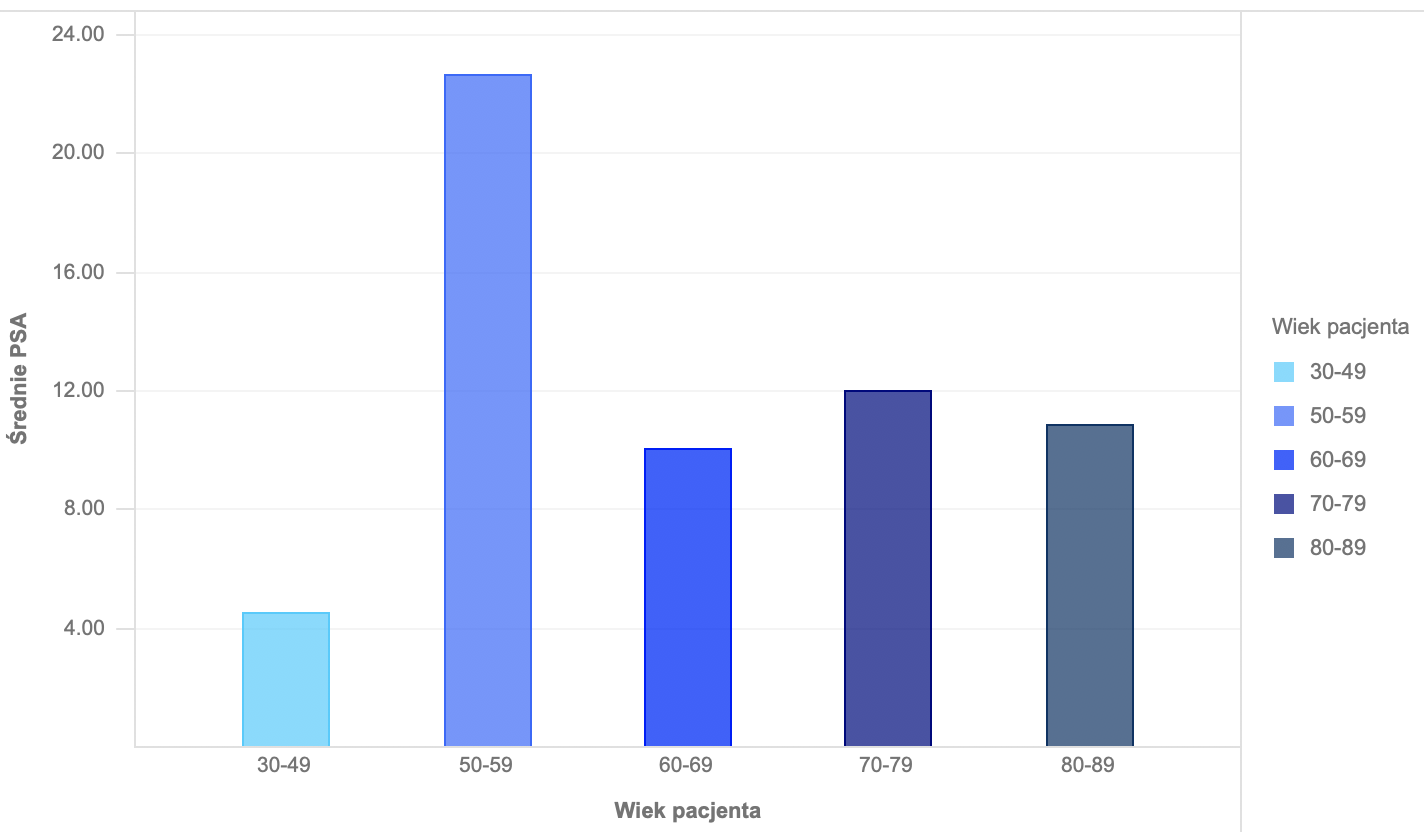
\includegraphics[width=\textwidth]{Wykresy/AgePSA.png}
	\captionof{figure}{PSA względem wieku}
\end{minipage}
\\
Wiek pacjentów został pogrupowany. Widać, że największe średnie PSA mają mężczyźni między 50 a 60 rokiem życia. Jest to obserwacja, którą dało się przewidzieć, ponieważ mężczyźni często dopiero zaczynają się badać po 50. roku życia. 
\\
Następnie chcieliśmy sprawdzić czy istnieje korelacja pomiędzy poziomem PSA i wynikiem uzyskanym w skali Gleasona.
\\
\begin{minipage}{\linewidth}
	\centering
	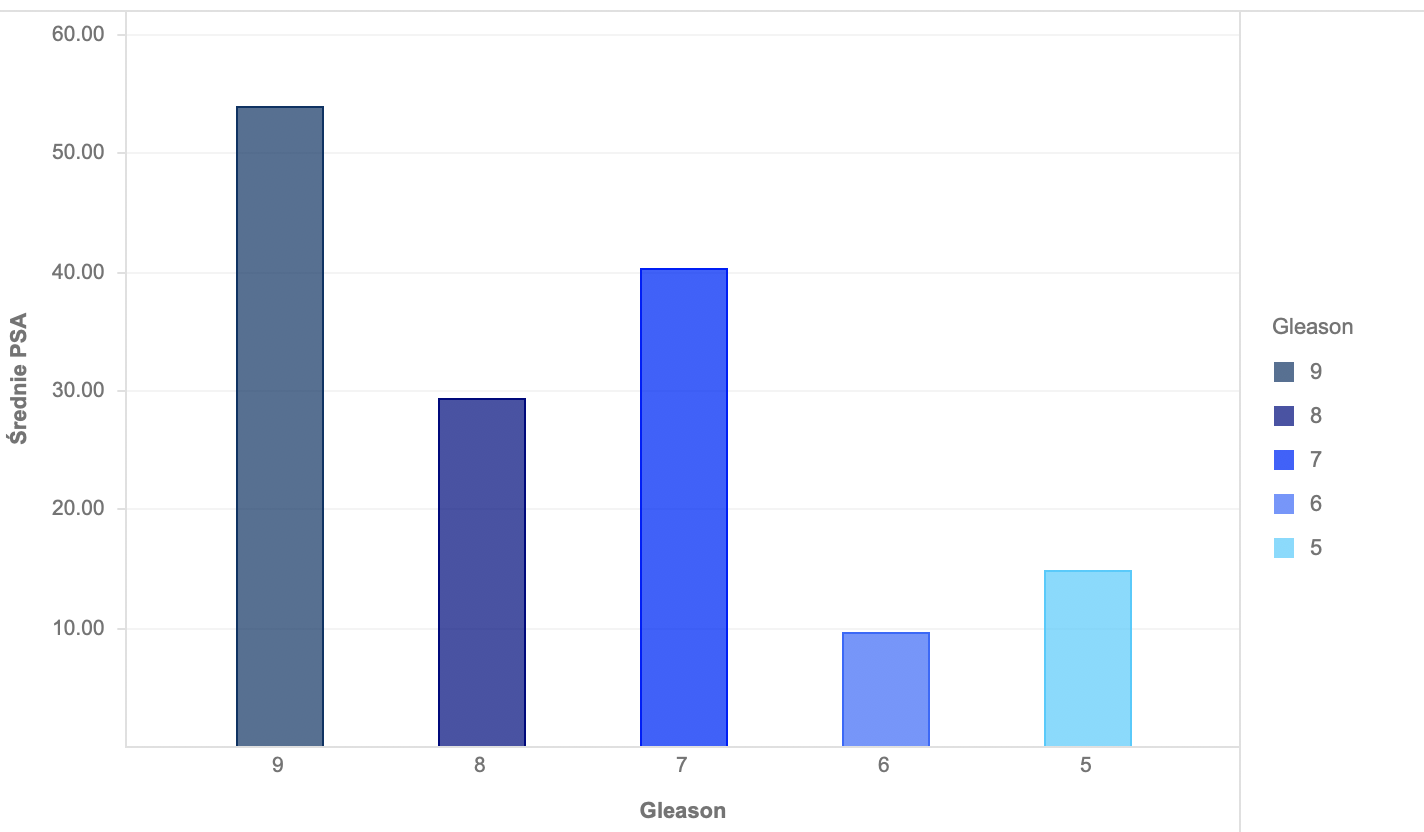
\includegraphics[width=\textwidth]{Wykresy/PSAGleason.png}
	\captionof{figure}{PSA względem Gleasona}
\end{minipage}
\\
U dwóch badanych pacjentów zdiagnozowano raka z oceną Gleasona na poziomie 9. Średnie PSA tych pacjentów wynosiło ponad 50 ng/ml co jest pięćdziesięciokrotnym przekroczeniem normy.
\\
Kolejnym badaniem jakie przeprowadziliśmy było sprawdzenie powiązania czy PSAD rośnie wraz z punktacją Gleasona
\\
\begin{minipage}{\linewidth}
	\centering
	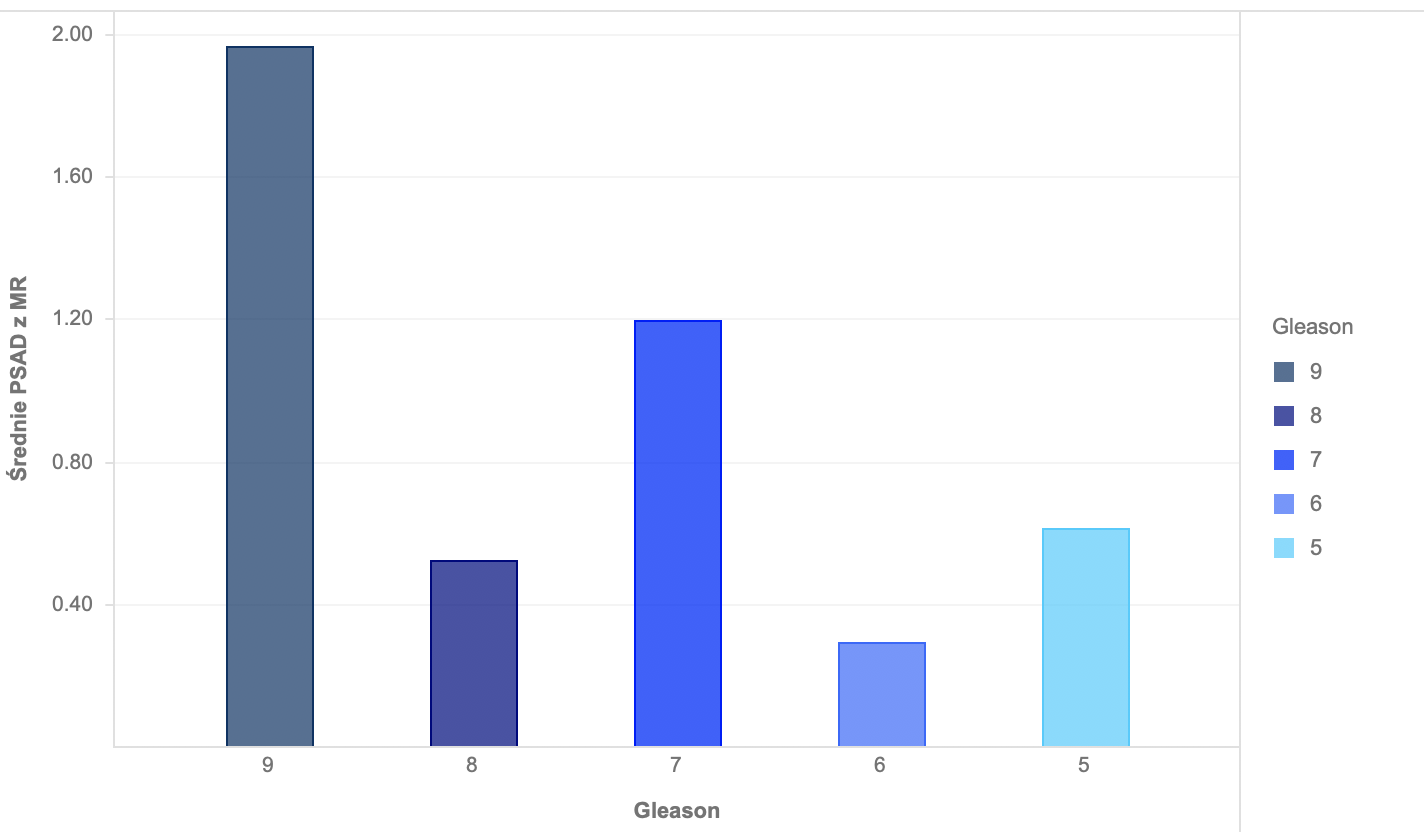
\includegraphics[width=\textwidth]{Wykresy/PSADGleason.png}
	\captionof{figure}{PSAD względem Gleasona}
\end{minipage}
\\
Na tym wykresie można zobaczyć Jak skala Gleasona wpływa na PSAD, czyli połączenie PSA oraz objętości prostaty. 
\\
Ostatnim testem było sprawdzenie czy istnieje zależność pomiędzy PSA oraz PIRADS.
\\
\begin{minipage}{\linewidth}
	\centering
	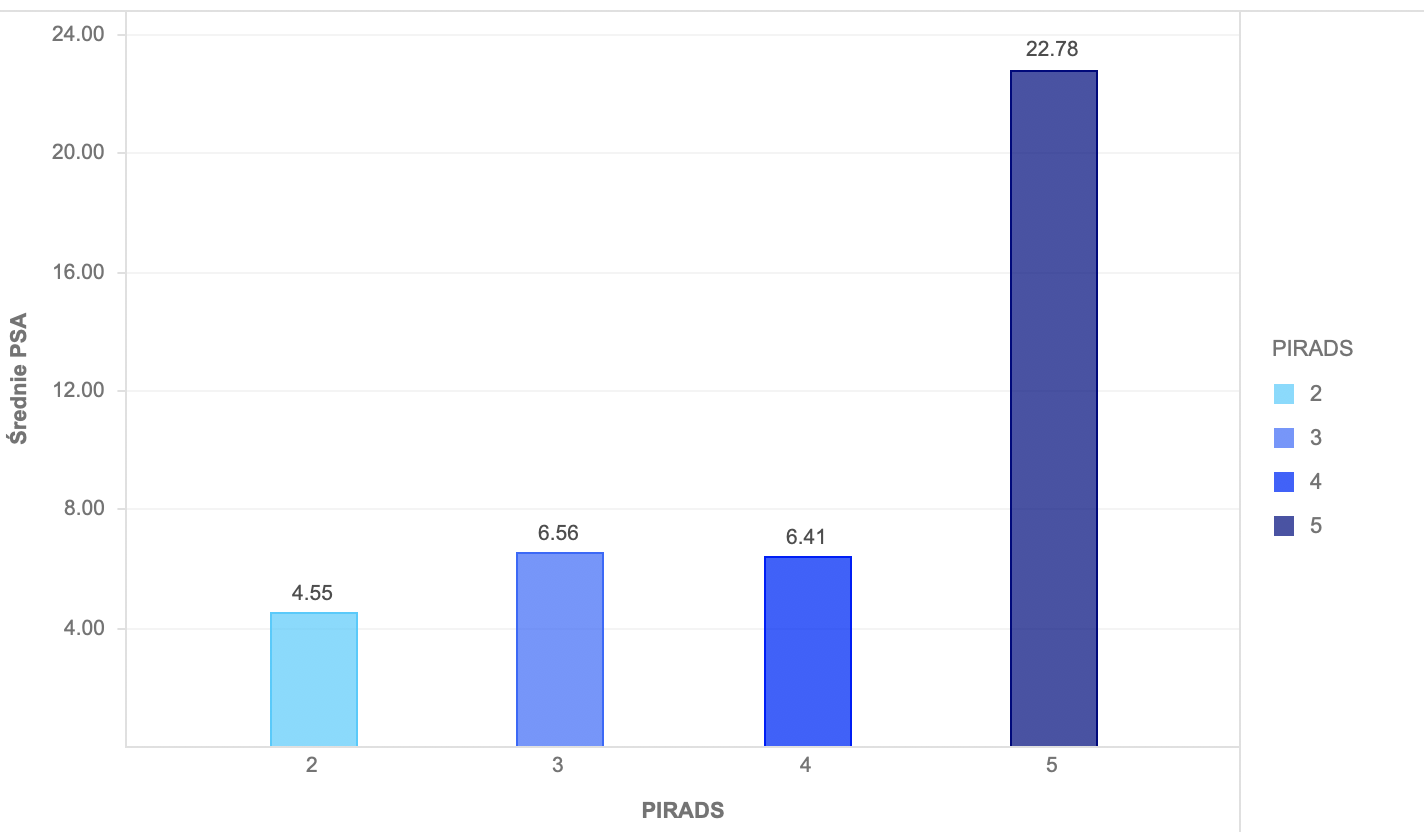
\includegraphics[width=\textwidth]{Wykresy/PIRADSPSA.png}
	\captionof{figure}{PSA względem PIRADS}
\end{minipage}
\\
Na wykresie poziomy PIRADS 2,3 i 4 mają stosunkowo podobne wyniki średniego PSA, natomiast poziom PIRADS 5 ma zdecydowanie zawyżony poziom PSA. 


\section{Ciekawe przypadki}
Podczas analizy danych pacjentów udało się zidentyfikować trzy najbardziej interesujące przypadki. Kryterium wyboru ich ciekawości było czysto subiektywne. Przypadki opisane są za pomocą identyfikatora PW, który został nadany pacjentom w celu anonimizacji ich danych.
\par
\begin{description}
\item  PW86 - PSA na poziomie 483,3 ng/ml, najwyższe dotychczas spotkane. Podwyższone PSA, oczywiście jest następstwem raka znalezionego w obu płatach prostaty.
\item  PW35 - ognisko PI-RADS V2 o mocy 5 znalezione w prawym płacie prostaty, natomiast po biopsji stwierdzono raka w lewym płacie.
\item  PW143 - 65 wykonanych badań PSA. Na każdym z nich wynik jest podwyższony, natomiast ani badanie rektalne, ani MR ani biopsja nie wykazały obecności raka.
\end{description}


% -------------------- Opis rozwiązania -----------------------
\chapter{Specyfikacja} % Cel i założenia projektu

Celem pracy dyplomowej jest stworzenie narzędzia wspomagającego diagnostykę nowotworu prostaty. Powinno ono wspierać pracę lekarza w diagnozie oraz zapewnić automatyczne znajdowania prostaty na zdjęciach rezonansu magnetycznego. Priorytetem aplikacji jest to aby posiadała modularną strukturę, która zapewni łatwą integracja ze szpitalną bazą danych oraz szybki rozwój lub zamianę istniejących komponentów. Aplikacja aby zapewnić łatwy dostęp do szpitalnych baz danych musi posiadać komponent odpowiadający za integrację z systemem PACS. Na potrzeby poniższej pracy utworzyliśmy naszą instancję bazy danych w oparciu o otwarte rozwiązanie ORTHANC \cite{Orthanc} w celach deweloperskich.
\par
Narzędzie będzie w stanie przyjąć nowe dane pacjenta w formacie DICOM, przetworzyć zdjęcia zawarte w pliku, wykonać segmentację gruczołu prostaty oraz wyświetlić użytkownikowi przewidywaną maskę. Ponadto użytkownik jest w stanie samodzielnie modyfikować predykcję maski używając do tego opcji edycji. W takim wypadku jako segmentacja zostaje zapisana najnowsza wersja maski stworzonej przez lekarza. Dzięki temu w ramach prowadzonej diagnostyki przeprowadzanej przez specjalistów powstają wysokiej jakości zbiory danych potrzebne do wprowadzenia metod wspomagania opartych o narzędzia sztucznej inteligencji. Kolejny moduł to moduł liczenia objętości wysegmentowanego gruczołu. Aplikacja powinna zapewniać kilka alternatywnych algorytmów obliczania, dzięki czemu będziemy mogli porównywać otrzymane wyniki.
\par
Ponieważ chcemy dostosować aplikację pod jak największą ilość środowisk, serwer backendowy powinien być możliwy do instalacji na każdym systemie operacyjnym.

\section{Opis biznesowy}

Aktualnie jest dostępnych wiele przeglądarek formatu DICOM, lecz żadna z nich nie zawiera modułu pozwalającego na segmentację gruczołu prostaty. Jedną z ważniejszych informacji jakie wykorzystuje się przy diagnostyce raka gruczołu prostaty jest objętość. Na tej podstawie szacuje się parametr PSAD, który silniej niż w przypadku PSA koreluje z obecnością nowtworu w prostacie. Ponadto, żadne z narzędzi używanych obecnie w szpitalu nie posiada modułu pozwalającego na liczenie objętości gruczołu.
\par
Nasze rozwiązanie ułatwia pracę lekarza przedstawiając aproksymowaną objętość gruczołu prostaty. Dodatkowo użytkownik jest w stanie samodzielnie poprawić predykcję używając opcji edycji maski. Dzięki takiej informacji wraz z rozwojem systemu mamy dostęp do coraz dokładniejszych danych dotyczących segmentacji pacjenta. Aplikacja ułatwi pracę lekarza oraz zgromadzi dane zawierające dokładne segmentacje utworzone przy użyciu algorytmu, które następnie podlegają kontroli lekarza. Narzędzie dostarcza również informacje na temat objętości gruczołu krokowego biorąc pod uwagę precyzję urządzenia na którym zostały wykonane zdjęcia. 
\par
Objętość jest kluczową informacją dla lekarza przy wystawianiu diagnozy. Wizualizacja wysegmentowanego gruczołu prostaty oraz obliczona wartość objętości pomoże lekarzowi w diagnostyce, a dzięki łatwemu rozszerzaniu aplikacji rozwój i modyfikacje modułu obliczania objętości lub segmentacji można łatwo zmieniać algorytmy, za pomocą, których je wyznaczamy.

\section{Wymagania funkcjonalne}

Podstawowym wymaganiem aplikacji jest możliwość liczenia segmentacji, objętości oraz integracja ze szpitalnym systemem PACS. Metody realizacji każdego z nich zostały opisane w dalszej części pracy. 

Podstawą interakcji użytkownika z systemem jest strona WWW - użytkownik powinien
być w stanie otworzyć ją na dowolnym komputerze z dostępem do internetu, wyposażonym
w przeglądarkę:
\begin {enumerate}
\item Google Chrome w wersji 49 lub wyższej
\item Mozilla Firefox w wersji 52 lub wyższej
\item Safari w wersji 10.1 lub wyższej
\end {enumerate}
Posiadanie przeglądarki innej niż wymienione lub w starszej wersji nie oznacza że strona nie będzie działać, jednak nie da się zagwarantować że będzie to działanie w pełni poprawne.
Każdy z użytkowników ma dostęp do tych samych danych oraz takie same możliwości
Funkcjonalność aplikacji WWW rozbita jest na trzy podstrony:
\begin {enumerate}
\item Wyświetlenie listy dostępnych pacjentów z aplikacyjnej bazy danych lub ze szpitalnego systemu PACS po wpisaniu danych logowania lekarza.
\item Dodanie nowego pacjenta z pliku lub ze szpitalnej bazy danych. Dane szpitalne przed wysłaniem na stronę serwera powinny być zanonimizowane tak aby serwer nie przechowywał żadnych danych wrażliwych.
\item Wyświetlenie danych pacjenta w tym obrazu z rezonansu magnetycznego, maski uzyskanej poprzez segmentacje obrazu, danych z pliku DICOM oraz wartości objętości gruczoły na podstawie aktualnej maski.
\end {enumerate}

\section{Diagram przypadków użycia}

Po wejściu na stronę internetową wyświetlana jest lista pacjentów znajdujących się obecnie w bazie danych. Dodatkowo po wcześniejszym połączeniu się z systemem szpitalnym PACS ma możliwość wyświetlenia pacjentów ze szpitalnej bazy danych. W ramach środowiska deweloperskiego dane, którymi inicjalnie zasilona jest aplikacyjna baza danych pochodzą z konkursu. \cite{konkurs}
Lekarz ma możliwość dodania nowego pacjenta z pliku lub ze szpitalnej bazy danych. Aby dodać pacjenta z pliku wystarczy w przeglądarce wybrać pacjenta, obraz DICOM zostanie pobrany z bazy PACS aplikacja, zanonimizowany po stronie przeglądarki, a następnie wysłany do serwera. Dodatkowo użytkownik ma możliwość dodania pacjenta z pliku DICOM poprzez przeciągnięcie zbioru zdjęć pacjenta na okno przeglądarki. W przypadku gdy wybrany pacjent nie znajduje się jeszcze w bazie danych aplikacja tworzy nowa encję opisującą tego pacjenta, w przeciwnym przypadku, jeżeli obraz nie znajduje się jeszcze w bazie danych dla pacjenta o takim identyfikatorze, aplikacja dodaje kolejne zdjęcia dla już istniejącego pacjenta.
Następnie lekarz ma możliwość oglądania zdjęć pacjenta, oraz danych jakie o tym pacjencie aktualnie znajdują się w bazie danych. Strona wyświetla kolejne obrazy, które zostały dodane dotyczące wybranego przypadku. Dodatkowo wyświetlane są informacje z pliku DICOM dotyczące informacji o pacjencie i wyników badań jeżeli taki znajdowały się w pliku, który  został wysłany do bazy danych. Ponadto aplikacja wyświetla maskę przedstawiającą wynik procesu segmentacji prostaty. Użytkownik ma możliwość ukrycia maski oraz jej edycji za pomocą dostarczonych narzędzi. 
Aplikacja dodatkowo liczy objętość wysegmentowanej prostaty na podstawie masek znajdujących się w bazie danych. W aplikacji dostępne jest kilka alternatywnych algorytmów liczenia objętości. Wartość nie jest przeliczana automatycznie w przypadku edycji. Lekarz po edycji wszystkich masek, naciska przycisk na stronie, który uruchamia proces liczenia objętości 
\par
Na poniższym rysunku przedstawiono w postaci diagramu UML zbiór przypadków użycia platformy dla lekarza i dla administratora systemu (programisty).
\par
\begin{minipage}{\linewidth}
	\centering
	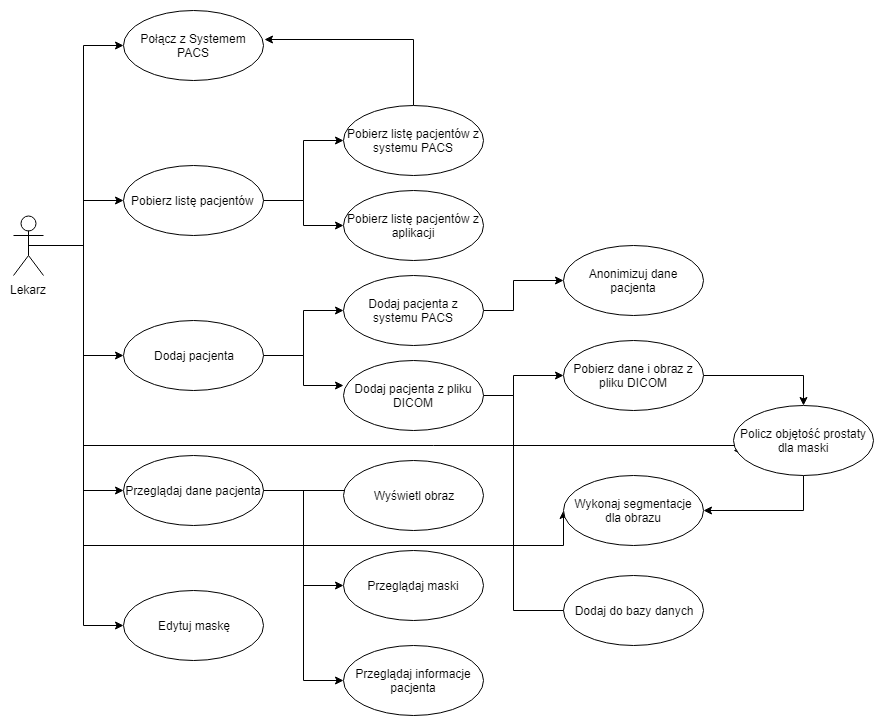
\includegraphics[width=0.5\textwidth]{useCase.png}
	\captionof{figure}{Diagram przypadków użycia}
\end{minipage}
\par

W tabeli \ref{Przypadki użycia} zebrano szczegółowe opisy przypadków użycia.

\begin{table}[h!]
\caption{Przypadki użycia}
\centering
\begin{tabular}{|p{3cm}|p{7cm}|p{6cm}|} \hline 
	Nazwa & Opis & Odpowiedź systemu \\ \hline 
	Połącz z systemem PACS & Użytkownik po podaniu informacji dostępu do szpitalnego systemu PACS zostaje z nim połączony & Lista pacjentów znajdujących się w wybranym systemie \\ \hline 
	Pobierz pacjenta z systemu PACS & Pobranie obrazu lub obrazów w formacie DICOM i wysłanie ich po uprzedniej anonimizacji do serwera aplikacyjnego & Informacja o sukcesie lub błędzie przy dodawaniu użytkownika \\ \hline 
	Dodaj pacjenta z pliku & Wysłanie pliku lub plików DICOM do serwera aplikacyjnego & Informacja o sukcesie lub błędzie przy dodawaniu użytkownika \\ \hline 
	Wyświetl listę pacjentów dostępnych w systemie & Pobiera listę pacjentów dostepnych w systemowej bazie danych, inicjalnie baza danych jest zasilona danymi pochodzącymi z archiwum danych pacjentów ze zdiagnozowanym rakiem prostaty & Lista identyfikatorów dostępnych pacjentów \\ \hline 
	Zobacz pacjenta & Wyświetla dane dotyczące danego pacjenta aktualnie znajdujące się w bazie danych, w szczególności listę obrazów rezonansu magnetycznego oraz maskę z wysegmentowaną prostatą & Dane pacjenta \\ \hline 
	Segmentuj & Oblicza segmentację dla wybranego obrazu & Maska opisująca prostatę na wybranym obrazie \\ \hline 
	Policz objętość & Liczy objętość na podstawie listy masek na podstawie wybranego algorytmu & Wartość objętości prostaty\\ \hline 
\end{tabular}
\label{Przypadki użycia}
\end{table}

\section{Wymagania niefunkcjonalne}

Tabla \ref{Wymagania niefunkcjonalne} przedstawia wymagania niefunkcjonalne w naszym systemie.

\begin{table}[h!]
\caption{Wymagania niefunkcjonalne}
\centering
\begin{tabular}{|r|r|p{10cm}|} \hline 
	Obszar wymagań & Nr wymagania & Opis \\ \hline 
	Użyteczność & 1 & Aplikacja będzie aplikacją internetową dostępną na systemach Linux lub Windows. Aplikacja będzie zawierać przyjazne użytkownikowi karty z opcją segmentacji oraz obliczania objętości prostaty. Dodatkowo lekarz będzie miał możliwość dodawania kolejnych pacjentów \\ \hline 
	Niezawodność & 2 & Aplikacja będzie w stanie wykonywać funkcjonalności opisane wyżej. Ponadto Aplikacja będzie zapisywać logi z błędami oraz przyczyną awarii \\ \hline 
	Wydajność & 3 & Aplikacja WWW powinna działać płynnie na każdym
komputerze z dowolnym systemem operacyjnym wyposażonym
w odpowiednią przeglądarkę. Obliczenia zależnie od rozmiarów danych wejściowych aplikacja powinna wykonywać takim czasie aby praca użytkownika nie była przez nią spowolniona, przy tym nie blokując interfejsu użytkownika \\ \hline 
	Utrzymanie & 4 & Aplikacja będzie miała architekturę modułową, która będzie łatwo rozszerzalna. Cały kod aplikacji zostanie udokumentowany. W ramach środowiska developerskiego powstanie obraz Docker.  \\ \hline 
\end{tabular}
\label{Wymagania niefunkcjonalne}
\end{table}

\section{Środowisko sprzętowe i programowe}

Opiszemy w dużym skrócie technologie wykorzystane w poniższej pracy, decyzje jakie stały za poszczególnymi wyborami, oraz alternatywne technologie i przyczyny dlaczego się na nie nie zdecydowaliśmy. 

\subsubsection{Języki i technologie }

\begin{description}
\item [Docker] \hfill \\
Podstawą całej architektury backendowej aplikacji jest wykorzystanie kontenerów czyli środowiska, w którym każdy serwis uruchamiany jest w odizolowanym środowisku zawierającym wszystkie zależności wymagane do jego działania. Ponieważ każdy z nas miał inne środowisko deweloperskie, Docker zapewnia nam, że serwisy będą działały w dokładnie ten sam sposób na każdej maszynie. Ma to również zalety dla środowisk produkcyjnych, ponieważ niezależnie czy udostępnimy naszą aplikację jako program on-premise czy zdecydujemy się na umieszczenie go w chmurze, konfiguracja będzie tak samo nieskomplikowana. Zapewnia to niezależność poszczególnych komponentów oraz odizolowanie aplikacji od systemu operacyjnego. Zdecydowaną przewagą Docker’a nad wirtualizacją jest możliwość uruchomienia aplikacji w wydzielonym kontenerze, ale bez konieczności emulowania całej warstwy sprzętowej i systemu operacyjnego. Do zarządzania kontenerami użyliśmy udostępnianego przez Docker narzędzia docker-compose. W ten sposób w przypadku potrzeby modyfikacji jednego z serwisów, aplikacja dalej pozostaje aktywna a zmianie ulega tylko jeden moduł.
\item [Środowisko .NET Core] \hfill \\
Serwis backendowy, który odpowiada za integrację z bazą danych oraz komunikację z warstwą prezentacji został napisany przy użyciu frameworku .NET Core. Główną zaleta tego wyboru jest wieloplatformowość rozwiązania. Dzięki nowemu środowisku uruchomieniowemu aplikacja może działać na dowolnym systemie operacyjnym. Korzystamy z najnowszej na chwilę pisania pracy wersji (2.1), która wspiera większość pakietów dostępnych dla .NET Framework. Dodatkowo głównym założeniem przy powstawaniu systemu było aby był oparty o architekturę mikroserwisów przy użyciu kontenerów, które również są wspierane przez framework.
\item [Język programowania C\# ] \hfill \\
System został wykonany z wykorzystaniem języka programowania C\# oraz platformy programistycznej .NET Framework. Wybór tej technologii był podyktowany doświadczeniem zespołu w jej wykorzystaniu. .NET Framework został wykorzystany do napisania modułu backendowego odpowiedzialnego za obsługę akcji użytkownika oraz komunikację z bazą danych. Ponieważ serwer powinien działać na wszystkich systemach operacyjnych użyliśmy .NET core oraz ASP.NET MVC Core.
\item [Entity Framework Core] \hfill \\
Entity Framework Core jest dedykowanym framework'iem dla aplikacji działających w środowisku .NET Core zapewniający dostęp i zarządzanie bazą danych. Jest to narzędzie typu ORM (ang. Object RelationalMapping). Dzięki użyciu tego narzędzia jako warstwy dostępu do bazy danych mogliśmy w łatwy sposób stosować podejście code-first przy projektowaniu aplikacji. Dodatkowo w przeciwieństwie do wersji z .NET Framework Entity Framework zapewnia wydajność porównywalną do natywnych wywołań zapytań bazodanowych za pomocą dedykowanego sterownika dla .NET czyli ADO.NET.
\item [SQL Server 2016] \hfill \\
Microsoft SQL Server jest systemem służącym do zarządzania bazą danych stworzonym przez firmę Microsoft. Platforma spełnia wszystkie podstawowe funkcjonalności jakich oczekujemy od bazy danych ale dodatkowo ponieważ w przypadku operowania na dużych wolumenach danych, co jest bardzo prawdopodobne w przypadku danych szpitalnych, oferuje wiele możliwości optymalizacji oraz zaawansowane narzędzia do utrzymania oraz analityki. Jest to platforma preferowana do projektów działających w .NET Framework. Pomino stosowania w projekcie podejścia \textit{Code first} nie wykluczamy, że w przypadku rozwoju platformy będzie trzeba je zmienić.
\item [Język programowania Python ] \hfill \\
W aplikacji wykorzystaliśmy język Python do modułu odpowiadającego za segmentację prostaty na obrazie. Wybór ten podyktowany jest dużą ilością dostępnych pakietów do uczenia maszynowego oraz głębokiego uczenia. Python jest wspierany na wszystkich większych systemach operacyjnych oraz łatwo tworzy się kontenery wykorzystujące Pythona. Ponadto brak procesu kompilacji wspomagał proces prototypowania algortytmu, co w przypadku uczenia maszynowego ma duże znaczenie. 
\item [Framework Flask ] \hfill \\
Aby zapewnić komunikację za pomocą protokołu http między serwisem segmentacji, a pozostałymi elementami systemu potrzebowaliśmy biblioteki, która udostępnia taką funkcjonalność.Framework zapewnia elementarną implementacją serwera http, który pozwala na komunikację z pozostałymi komponentami. Ponieważ segmentacja wspiera tylko i wyłącznie jeden punk dostępowy uznaliśmy, że wybór rozwiązania bardziej rozbudowanego jest nieuzasadniony. Django czy Pyramid, to dwa bardzo popularne rozwiązania dla serwerów http zaimplementowane w języku Python jednak o wiele bardziej rozbudowanej konfiguracji nie przynosząc zarazem odczuwalnych korzyści.
\item [Biblioteka Keras] \hfill \\
Do implementacji algorytmu segmentacji gruczołu krokowego na zdjęciach potrzebowaliśmy biblioteki pozwalającej na tworzenie sieci neuronowych. Podczas poszukiwań najbardziej odpowiedniego rozwiązania kierowaliśmy się kilkoma kryteriami. Przede wszystkim chcieliśmy aby rozwiązanie było napisane w języku Python oraz wspierało użycie biblioteki TensorFlow. Dodatkowo chcieliśmy aby biblioteka umożliwiała szybkie prototypownie oraz była przenośna między systemami operacyjnymi. Keras jest obecnie jednym z najpopularniejszych bibliotek do takiego zastosowania. Zapewnia wysoko poziomowy interfejs ułatwiający tworzenie rozwiązań opartych o uczenie maszynowe. Decyzja o użyciu frameworku zapadła na podstawie spełniania wszystkich powyższych założeń oraz doświadczeniem zespołu w jego wykorzystaniu.
\item[Tensorflow] \hfill \\
TensorFlow jest biblioteką typu otwarty kod do obliczeń numerycznych i uczenia maszynowego. Biblioteka łączy ze sobą szereg modeli i algorytmów głębokiego uczenia. Korzysta z Pythona, aby zapewnić wygodne API do budowania aplikacji, a obliczenia wykonywane są w C ++. Biblioteki nie wykorzystaliśmy bezpośrednio tylko przez nakładkę Keras, która udostępnia wysokopoziomowe API.
\item [OpenCV, OpenCvSharpCore] \hfill \\
OpenCV \cite{OpenCV} to biblioteka oprogramowania do nauki i uczenia maszynowego typu open source. Jest to chyba najpopularniejsza biblioteka do przetwarzania obrazów. Do integracji z .NETem użyliśmy wrappera działającego w środowisku .NET Core OpenCVSharpCore. Zapewnia dostęp do metod biblioteki poprzez kod C\#. W naszej pracy została wykorzystana w module liczącym objętość do znajdowania otoczki maski oraz liczenia pola powierzchni poligonów.
\item [React] \hfill \\
  React okazał się idealnym rozwiązaniem, ponieważ jest jedynie biblioteką dostarczającą komponenty, która może być rozszerzalna przez kolejne biblioteki. Projekt ten dojrzałym framework'iem stworzonym i rozwijanym przez Facebook. Przygotowując aplikację SPA postanowiliśmy znaleźć rozwiązanie, które najbardziej dopasuje sie do naszych wymagań. 
\end{description}

Ponadto wszystkie wymienione technologie zostały wybrane do realizacji pracy, ponieważ zespół, który nad nią pracował, miał doświadczenie w pracy z nimi wyniesione z poprzednich projektów realizowanych w ramach studiów i pracy zawodowej.

\subsubsection{Rozważane alternatywne technologie}
W momencie pisania pracy ustaliliśmy, że najpopularniejszymi aktualnie rozwiązaniami są następujące projekty:
	  
\begin{description}
	\item [Java] \hfill \\
	Jeden z najpopularniejszych obecnie języków programowania, teoretycznie spełniający wszystkie nasze wymagania. Zapewnia modularność, jest wspierany przez wszystkie języki programowania, ma wiele dostępnych bibliotek gotowych do użycia w aplikacji. Odrzuciliśmy ten wybór z powodu dużej ilości konfiguracji potrzebnej do utworzenia systemu jaki tutaj opisujemy. Dodatkowo ponieważ przetwarzamy pliku zajmujące często nawet powyżej 100MB obawialiśmy się problemów z wydajnością zwalniania pamięci w Javie. W przypadku przetwarzania dużych wolumenów danych Java wymaga dużej ingerencji w mechanizm zwalniania pamięci.
\item[Angular] \hfill \\
  	Projekt Angular jest jednym z najpopularniejszych obecnie rozwiązań do tworzenia warstwy prezentacji aplikacji. Początkowo wydawał się być doskonałym wyborem dla naszego zastosowania (dojrzały projekt, wspierany przez Google), aczkolwiek wymuszał on używanie konkretnych rozwiązań stworzonych na potrzeby tego konkretnego frameworka do wykonywania zapytań. Z tego powodu zdecydowaliśmy się zrezygnować z tego projektu, ponieważ naruszał nasze kryterium dotyczące modularności.
\item[Vue] \hfill \\
	Vue jest coraz bardziej popularnych frameworkiem, który wyróżnia się modularnością, przenośnością oraz niskim progiem wejścia. Nie dopasował się do naszych wymagań ze względu na niedojrzałość projektu, przez co dostępne komponenty nie spełniały naszych oczekiwań. Wciąż jest to rozwiązanie nie wspierane przez dużych klientów biznesowych.
\end{description}

% -------------------- Opis aplikacji -----------------------
\chapter{Opis aplikacji}
W tym rozdziale przedstawione zostaną efekty pracy. Na wstępie przedstawimy wysoko poziomową architekturę całego rozwiązania. Następnie opiszemy poszczególne moduły zawarte w aplikacji oraz zasadę ich działania, przedstawiając szczegóły techniczne implementacji. Dzięki podziałowi aplikacji na osobne serwisy działające niezależnie, zawarte w dalszej części opisu modułów również opiszemy niezależnie. Kontenery oddzielają aplikacje od siebie oraz infrastruktury, na której działają zapewniając dodatkową warstwę ochronną dla aplikacji.

\section{Architektura systemu}

System składa się z modułów realizujących ściśle określone zadania, niezależne zadania, dlatego też łatwo wydzielić je jako osobne serwisy działające niezależnie od siebie. Każdy z serwisów działa jako osobny kontener. Konteneryzacja polega na tym, że umożliwia się uruchomienie wskazanych procesów aplikacji w wydzielonych obiektach, które z punktu widzenia aplikacji są odrębnymi instancjami środowiska uruchomieniowego. Każdy kontener posiada wydzielony obszar pamięci, odrębny interface sieciowy z własnym prywatnym adresem IP oraz wydzielony obszar na dysku.

\begin{minipage}{\linewidth}
	\centering
	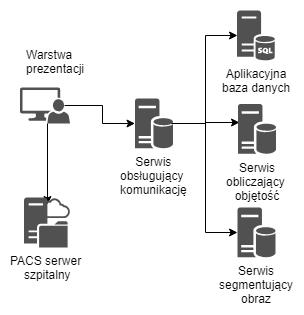
\includegraphics[width=0.5\textwidth]{Architektura.png}
	\captionof{figure}{Schemat architektury aplikacji}
\end{minipage}

Komunikacja serwera backendowego z serwerem PACS odbywa się za pośrednictwem aplikacji internetowej, z której korzysta klient. Jest to zrobione specjalnie i daje nam możliwość łatwej integracji z systemem szpitalny. W zasadzie jest to jedyna opcja jaką znaleźliśmy w trakcie naszego badania architektury szpitalnej nie wymagająca ustawiania specjalnego połączenia VPN między naszym serwisem a serwerami szpitalnymi. Dzięki temu zyskujemy niezależność. Aplikacja może działać na dowolnym środowisku przy tym zapewniając klientowi dostęp i wysyłanie danych pacjenta na nasze serwisy do przetwarzania.
Rozwiązanie w którym nasz serwer komunikuje się bezpośrednio z bazą danych szpitalnych ma kilka dużych wad. Przede wszystkim przesyłamy poufne dane pacjentów przez sieć. Aby to robić bezpiecznie potrzebowalibyśmy dedykowanego bezpiecznego połączenia, którego nie udało nam się uzyskać przez cały okres pisania pracy.
\par
Reszta architektury jest standardowa w przypadku aplikacji o architekturze mikroserwisowej. Mamy główny serwer odpowiadający za komunikację z użytkownikiem i obsługę bazy danych. Serwisy do liczenia objętości i segmentacji są niezależne i nie mają bezpośredniego dostępu do bazy danych.
Jedyna modyfikacja jaką można by wykonać w przypadku intensywnego użytkowania aplikacji to skonfigurować osobne bazy dla każdego serwisu aby uniknąć niepotrzebnego przesyłania danych przez sieć. Jednak w naszym przypadku proponowane rozwiązanie jest bezpieczniejsze, łatwiejsze w utrzymaniu i w zupełności wystarczające.

\section{Komunikacja między modułami}

Komunikacja między komponentami odbywa się za pomocą protokołu \textit{http}. Każdy z serwisów udostępnia swoje punkty dostępu. W przypadku serwisu kalkulującego objętość oraz wykonującego segmentację dostęp jest jedynie z poziomu kontenera.
\par
Serwisy są lokalizowane dzięki mechanizmom Dockera, który tworzy podsieć dla wszystkich działających w obrębie jednego Docker-compose. Dostęp do serwisów odbywa się przez adres postaci http://\textit{nazwa-serwisu}:\textit{port} (jeżeli nie zmieniony to serwis działa na porcie 80). Dostęp z zewnątrz zapewnia jedynie serwis obsługujący komunikacje, a pozostałe serwisy są niedostępne.
\par
Każdy z naszych serwisów udostępnia REST API. Najwięcej metod ma moduł do komunikacji z klientem, którego pełna dokumentacja jest opisana w Załączniku 1. Może być przydatne w przypadku chęci użycia naszego rozwiązania z inną warstwą prezentacji np. aplikacją okienkową.

\chapter{Opis modułów}

W poniższym rozdziale opiszemy poszczególne moduły. Wytłumaczymy drogę dojścia do rozwiązania oraz ewentualne modyfikacje jakie można zastosować przy dalszym rozwoju. Skupiliśmy się na unikaniu zależności pomiędzy modułami. Wszystkie moduły zaprojektowaliśmy w sposób modularny, tak aby dowolnie móc je wymieniać. 

\section{Moduł segmentacji}

Moduł odpowiada za znajdowanie na obrazie wejściowym prostaty. Algorytm działa na zdjęciach w formacie PNG i zwraca również obraz w tym samym formacie. Do obliczeń użyliśmy konwolucyjnych sieci neuronowych, na podstawie danych z konkursu \cite{konkurs}, które składały się  z obrazów badań MRI oraz wysegmentowanych masek przez specjalistów. Problem segmentacji gruczołu prostaty jest niezwykle istotny z perspektywy lekarzy, którzy na podstawie wysegmentowanej maski gruczołu są w stanie łatwiej postawić diagnozę dotyczącą raka prostaty.

\subsubsection{Segmentacja obrazu}

Segmentacja obrazu jest procesem dzielenia obrazu cyfrowego na wiele segmentów). Celem segmentacji jest uproszczenie i / lub zmiana reprezentacji obrazu na obszary, które są bardziej znaczące i łatwiejsze do analizy. Segmentacja obrazu jest używana do lokalizowania obiektów i granic (linii, krzywych itp.) w obrazach. Jest to proces przypisywania etykiety do każdego piksela na obrazie, tak że piksele z tą samą etykietą mają pewne cechy. Proces polega na podziale obrazu na  obszary, które są jednorodne pod względem pewnych wybranych cech. Przez obszar najczęściej rozumiemy zbiór pikseli obrazu. Zadanie segmentacji nie tylko wymaga zrozumienia co się znajduje na obrazie, lecz również ustalenia gdzie się ten obszar znajduje. Celem segmentacji jest wyeksponowanie  poszukiwanych własności obrazu, które są istotniejsze od pozostałych. Istnieje wiele algorytmów segmentacji, najpopularniejszymi są: progowanie obrazu, wykrywanie krawędzi, rozszerzanie obszaru. W przypadku każda z wyżej wymienionych metod jest zestawem reguł które są przygotowane przez człowieka podczas tworzenia algorytmu. Algorytmy te nie zależą w żaden sposób od danych na których będą wykonywać obliczenia. W ostatnich latach głębokie sieci neuronowe oraz konwolucyjne sieci neuronowe wykazały, że radzą sobie z problemem klasyfikacji lepiej niż statyczne rozwiązania.\cite{imageOrg}. Sieci na podstawie dużej ilości danych dobierają zestaw filtrów, który dajne najlepsze wyniki segmentacji dla danych treningowych. W naszej pracy postanowiliśmy zastosować sieci neuronowe, ponieważ rozwiązania oparte o głębokie uczenie od lat wygrywają konkursy na najlepsze wyniki  klasyfikacji oraz segmentacji. 

\subsubsection{Sieci neuronowe}

Głęboka sieć neuronowa (DNN) to sztuczna sieć neuronowa z wieloma warstwami między warstwami wejściową i wyjściową. DNN znajduje matematyczne przekształcenie, aby zmienić dane wejściowe na dane wyjściowe, niezależnie od tego, czy jest to relacja liniowa czy nieliniowa. Sieć przechodzi przez warstwy obliczające prawdopodobieństwo każdego wyjścia. Każda manipulacja matematyczna uważana za warstwę. Złożone głębokie sieci neuronowe mają wiele warstw. Celem jest, aby ostatecznie sieć została nauczona w zakresie rozkładania obrazu na funkcje, identyfikowania trendów istniejących we wszystkich próbkach i klasyfikowania nowych obrazów według ich podobieństw bez konieczności wprowadzania danych przez człowieka.
\par
Konwolucyjna  sieć neuronowa (CNN) to rodzaj sztucznej sieci neuronowej wykorzystywanej w rozpoznawaniu i przetwarzaniu obrazów, która jest specjalnie zaprojektowana do przetwarzania obrazów. W przeciwieństwie do sieci użytej do głębokiego uczenia maszynowego, każda ukryta warstwa aktywacyjna jest obliczany jako iloczyn kartezjański wyników kolejnych warstw. Jednak w sieciach konwolucyjnych każda ukryta aktywacja jest obliczana przez pomnożenie małego lokalnego sygnału wejściowego względem wag. Wagi są następnie dzielone na całej przestrzeni wejściowej. Po obliczeniu ukrytych jednostek, maksimum warstwa pomaga usunąć zmienność ukrytych jednostek. W szczególności każda jednostka gromadząca maksimum otrzymuje aktywacje ze znalezionej ilości splotowych pasm, i wyprowadza maksimum aktywacje z tych splotów. Większość CNN uzytych do rozpoznawania obrazu ma niższe warstwy sieciowe, które są splotowe, a wyższe warstwy sieciowe są w pełni połączone.

\subsubsection{U-Net}
Sieć U-Net jest zbudowana na podstawie architektury pełnych sieci konwolencyjnych(ang. Fully Convolutional Network) zmodyfikowaną w taki sposób, aby uzyskiwać lepsze rezulataty segmentacji na obrazach medycznych. Lepsze rezultaty pochodzą z kształtu architektury U, który skutkuje większą ilością cech w scieżce wstępującej co przekłada się na lepszy przepływ informacji o kontekście i lokalizacji na obrazach o niskiej rozdzielczości.

\begin{minipage}{\linewidth}
	\centering
	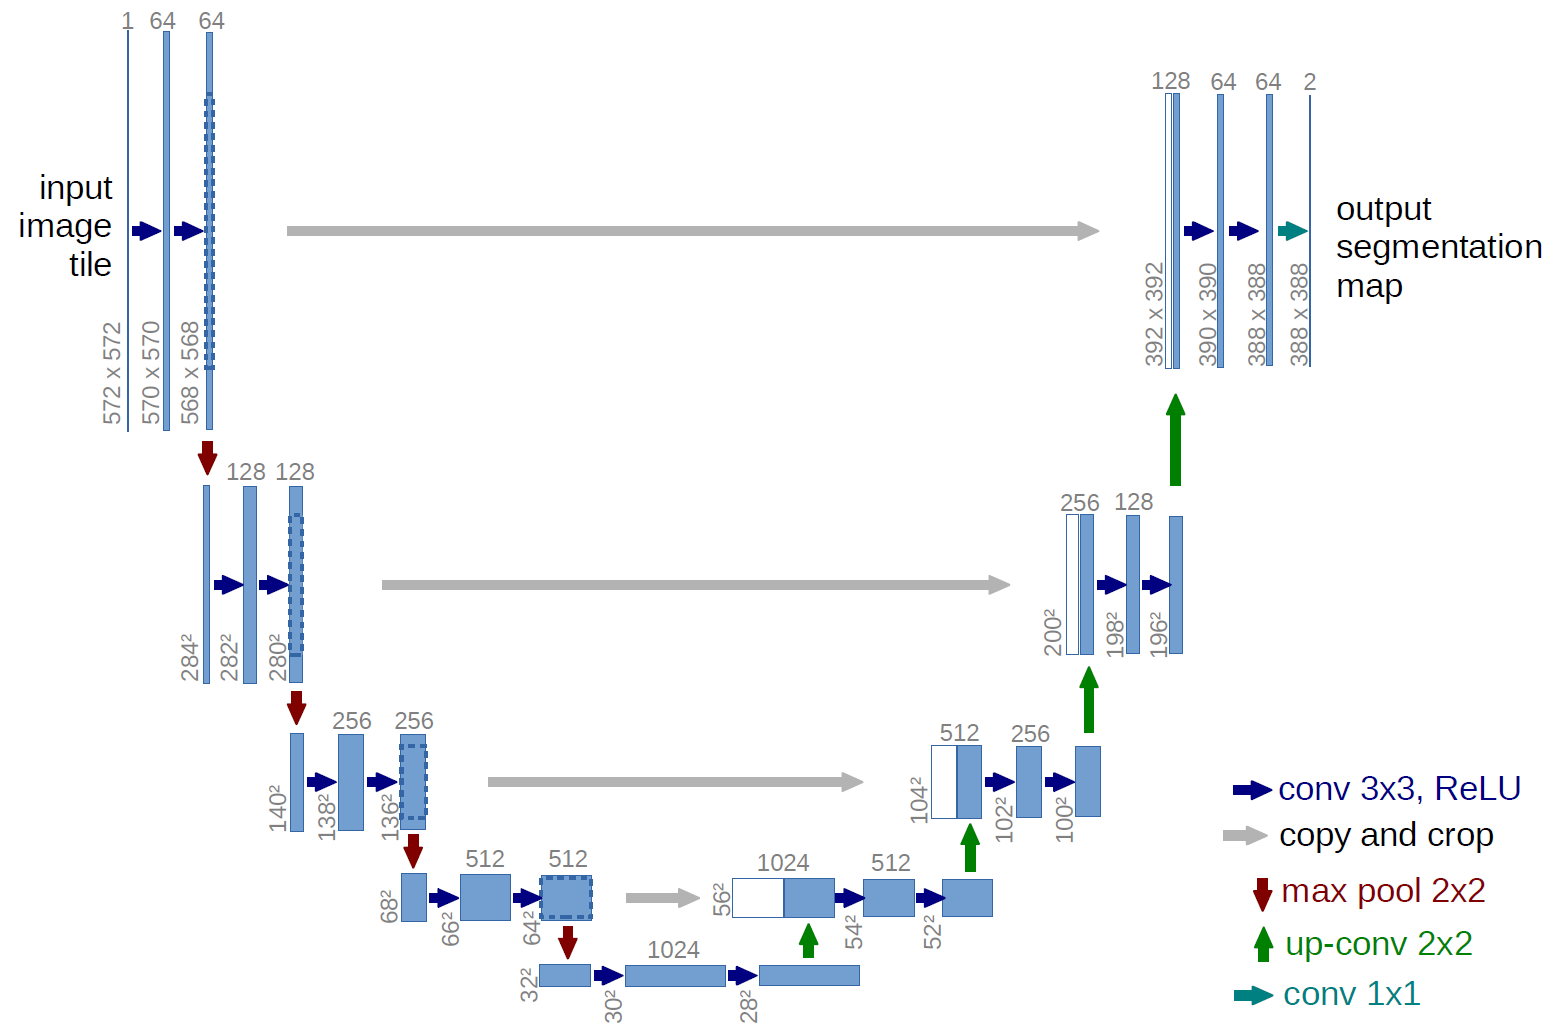
\includegraphics[width=10cm]{unet-architecture.png}
	\captionof{figure}{Architektura sieci UNet}
\end{minipage}


W procesie uczenia sieci neuronowych najbardziej czasochłonnym elementem jest proces trenowania. Uczenie sieci neuronowych odbywa się na kartach graficznych ze względu na ich lepsze przystosowanie do przetwarzania dużej ilości operacji w sposób równoległy. Procesor ma za zadanie przełączanie kontekstów, ale nie zapewnia wysokiej przepustowości. Musi przełączać się między wieloma zadaniami i przechowywać konteksty podczas przełączania i dbać o pamięć współdzieloną. Procesor może być wykorzystywany do zadań o niskiej przepustowości i wysokiej latencji. Z drugiej strony procesor graficzny został zaprojektowany z myślą o dużym obciążeniu pracą i wysokiej przepustowości.

\subsection{Opis danych}

Najlepszym źródłem pozyskania danych dla naszych celów badawczych są strony konkursowe ponieważ zawierają obrazy z już odnalezioną prostatą na zdjęciu. Organizowanych jest wiele konkursów \cite{konkurs} w celu opracowania stabilnego algorytmu wyznaczania gruczołu prostaty, jednak my po analizie zdecydowaliśmy się na dane z konkursu \textit{Automated Segmentation of Prostate Structures Challange} \cite{konkretny}.

\begin{description}
	\item [Dane] \hfill \\
	Dostarczone dane składały się z plików DICOM zawierających dane pacjentów oraz z maski zawierających obszary gdzie znajduje się prostata. Dane były przygotowane przez lekarzy, oraz podległy wcześniejszemu procesowi anonimazacji, stąd w plikach nie ma żadnych danych wrażliwych na temat pacjentów. Osoby poddano badaniom za równo pod maszynami o mocy 1.5T oraz 3T z użyciem cewki endorektalnej oraz cewki powierzchniowej. Maski zostały przygotowane  przez zespól lekarzy z uniwersytetów Boston University School of Medicine oraz Case Western University. Zdjęcia zostały przygotowane w formacie nrrd, gdzie zaznaczone są dwa regiony: część obwodową gruczołu krokowego (PZ) oraz centralny gruczoł(CG). 
	
	\begin{minipage}{\linewidth}
		\centering
		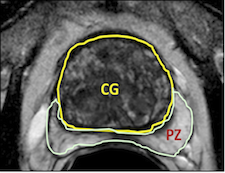
\includegraphics[width=0.5\textwidth]{segmentation/prostate_seg.png}
		\captionof{figure}{Zaznaczone regiony prostaty na zdjęciu z badania MR}
	\end{minipage}
	
	\begin{description}
		\item[Zbiór treningowy] 60 pacjentów, łącznie 1073 obrazów
		\item[Zbiór testowy] 10 pacjentów, 147 obrazów
		\item[Zbiór walidacyjny] 10 pacjentów, 146 obrazów
	\end{description}


	\item [Obrazy wejściowe] \hfill \\
	Dane zostały przetransformowane z formatu DICOM w taki sposób, aby wyeksportować tag pixelData i przekonwertować do postaci tablicy zawierającą tylko intensywność pixeli.
	
	\begin{minipage}{\linewidth}
		\centering
		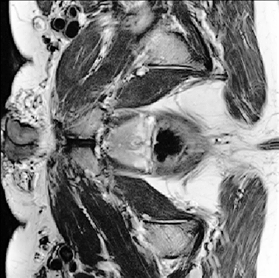
\includegraphics[width=0.5\textwidth]{segmentation/example_MRI_image.png}
		\captionof{figure}{Przykładowy obraz z badania MRI}
	\end{minipage}


	\item [Oznaczone maski] \hfill \\
Przygotowane maski podzielone zostały na dwa regiony gruczołu PZ oraz CG. Obszar CG został oznaczony wartościami 2, obszar PZ wartościami 1 natomiast pozostały obszar wartością 0.  Ponieważ nasz problemy był bardziej ogólny nie było potrzeby wprowadzenia rozróżnienia między strefami prostaty. Dlatego dane poddaliśmy procesowi normalizacji maski do wartości z przedziału [0;1].

\begin{minipage}{\linewidth}
	\centering
	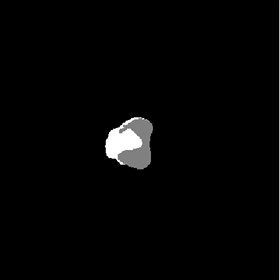
\includegraphics[width=0.5\textwidth]{segmentation/example_mask.png}
	\captionof{figure}{Przykładowy obraz z badania MRI}
\end{minipage}


\end{description}

\subsection{Opis rozwiązania}

W przypadku analizy obrazów medycznych problemem jest mały zbiór danych testowych dobrej jakości. Postanowiliśmy do tego celu wykorzystać dane pochodzące z konkursu opisane powyżej. Eksplorację danych rozpoczęliśmy od przeglądania obrazów DICOM. Na wstępie zauważyliśmy, że granice pomiędzy tkankami miękkimi nie są dobrze podkreślone. Co więcej dane jakie dostaliśmy są niskiej rozdzielczości. Segmentacja gruczołu krokowego nie jest zadaniem trywialnym z powodu podobnych intensywności obrazu między gruczołem prostaty a sąsiadującą tkanką oraz z powodu niejednorodności intensywności obrazu w okolicy prostaty. Co więcej, gruczoł krokowy ma dużą różnorodność wyglądu i kształtów u różnych pacjentów.
Z uwagi na bardzo ograniczony zbiór testowy zastosowaliśmy mechanizmy \textit{Data augmentation}, dzięki czemu w efektywny sposób zwiększyliśmy zbiór testowy. Rozwiązanie jest  procesem stosowanym przy przetwarzaniu obrazów medycznych, polega na zwielokrotnieniu zbioru testowego poprzez zastosowanie na obrazach inicjalnych podstawowych operacji przetwarzających obraz takich jak np. rotowanie obrazu, stosowanie filtru Gaussowskiego lub progowania.
\par
Przed wyborem rozwiązania przerowadziliśmy analizę aktualnie wykorzystywanych algorytmów do segmentacji obrazów. Jednym z założeń było znalezienie rozwiązania, które pomimo niewielkiego zbioru danych treningowych poradzi sobie z obrazami o niskiej rozdzielczości. Najbardziej dopasowanym rozwiązaniem okazała się uproszczona sieć U-net, która powstała jako zgłoszenie do konkursu Automated Segmentation of Prostate Structures \cite{zgloszenie}. Wybraliśmy te rozwiązanie ponieważ sieć jest symetryczna, dzięki czemu zyskujemy większą dokładność znajdowania regionów obrazu oraz pomija kilka warstw co skutkuje lepszymi rezultatami przy małej ilości danych. Rozwiązanie nauczyliśmy ponownie na danych opisanych w rozdziale powyżej. Architekturę sieci przedstawia poniższy diagram. 

\begin{minipage}{\linewidth}
	\centering
	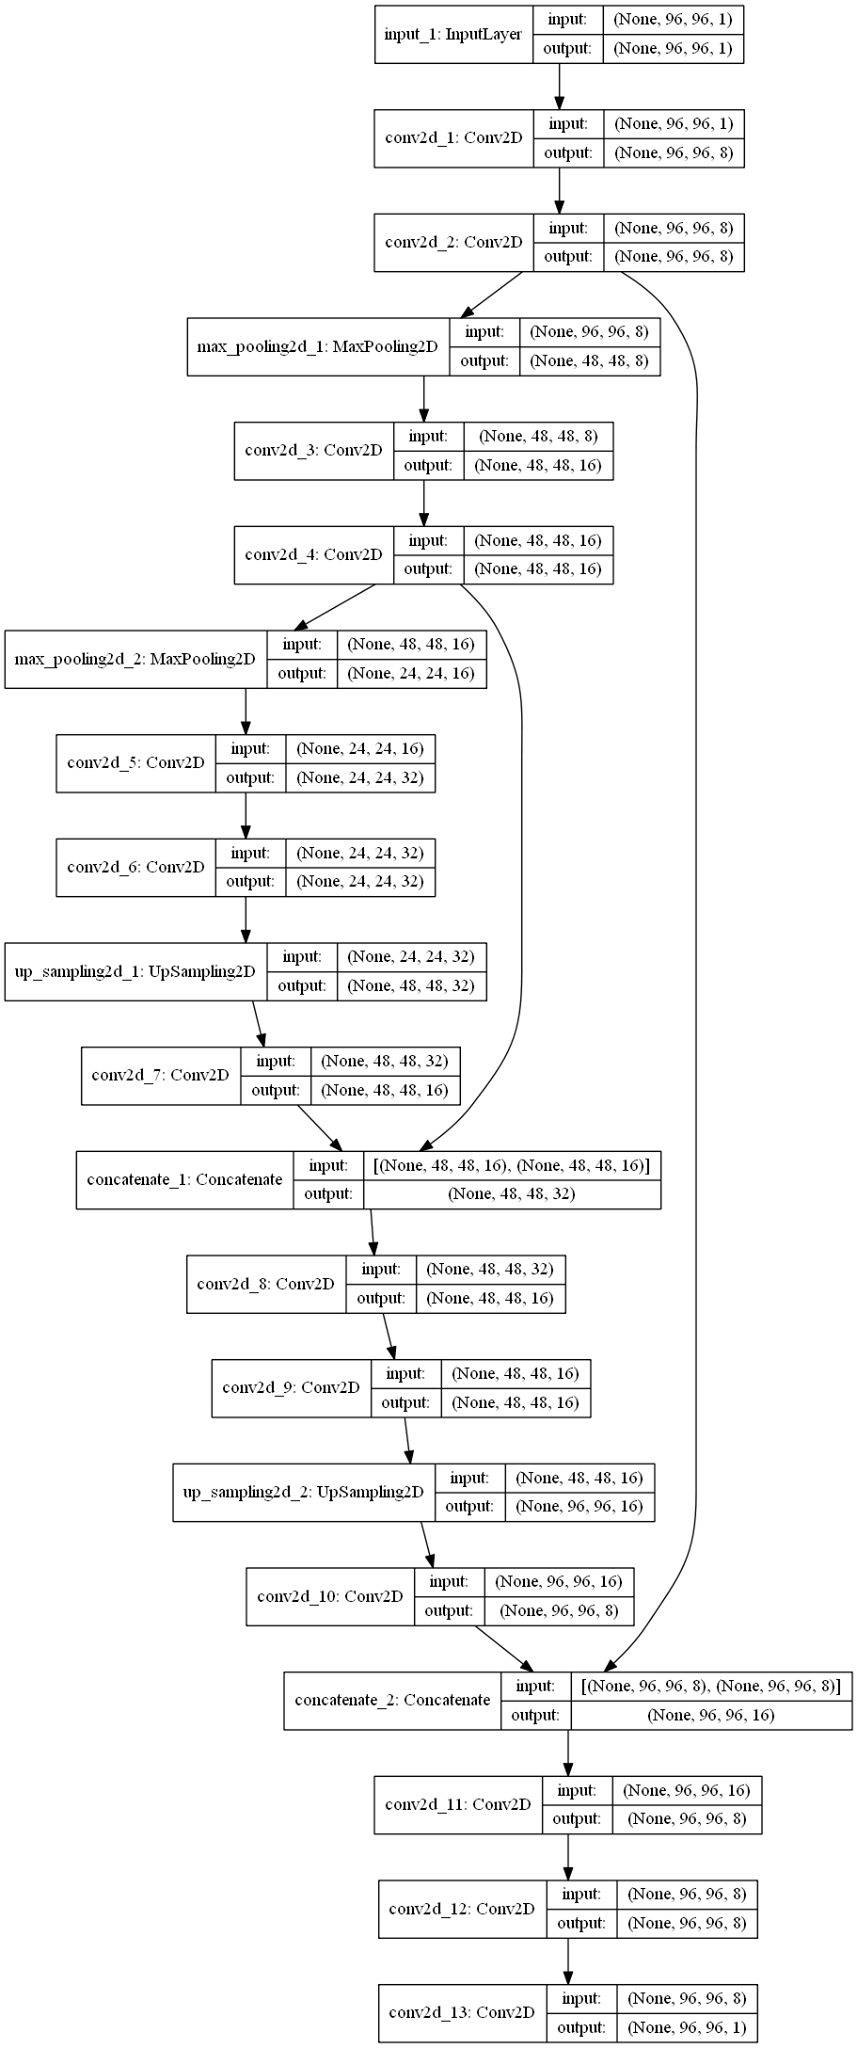
\includegraphics[width=0.65\textwidth]{segmentation/our_architecture.png}
	\captionof{figure}{Architektura sieci}
\end{minipage}


Architektura ta dzieli się na trzy części:

\begin{description}
	\item [Warstwa zstępująca] Zbiera informacje na temat kontekstu i znaczenia regionu. Interpretuje znaczenie obszaru poprzez zmniejszanie wielkości przestrzennej w każdym z bloku. Wszytkie bloki w tej ścieżsce składają się z następujących warstw:
	\begin{description}
		\item [Conv2D] 3x3 Warstwa konwolucyjna + funckja aktywacji ReLu
		\item [Conv2D] 3x3 Warstwa konwolucyjna + funckja aktywacji ReLu
		\item [MaxPooling2D]2x2 Max Pooling
	\end{description}
   Każdy blok podwaja liczbę konwolucji oraz zmniejsza rozmiar przestrzenny o  połowę.
	
	\item [Wąskie gardło] Znajduje się pomiędzy dwoma ścieżkami. Składa się z dwóch warstw konwolucyjnych
		\begin{description}
		\item [Conv2D] 3x3 Warstwa konwolucyjna + funckja aktywacji ReLu
		\item [Conv2D] 3x3 Warstwa konwolucyjna + funckja aktywacji ReLu
		\end{description}
	
	\item [Warstwa wchodząca] Składa się warstw powiększających dane przestrzenne regionu oraz jest łączona z symetrycznie odbitymi blokami ścieżki zstępującej co pozwala ustalić obszar oraz jego kontekst. Wszytkie bloki w tej ścieżsce składają się z następujących warstw:
	\begin{description}
		\item [UpSampling2D] 2x2 Warstwa powiększająca
		\item [Conv2D] 3x3 Warstwa konwolucyjna + funckja aktywacji ReLu
		\item [Concatenate] Połączenie informacji o lokalizacji przestrzennej z informacja o konteksie obszaru
		\item [Conv2d] 3x3 Warstwa konwolucyjna + funckja aktywacji ReLu
		\item [Conv2d] 3x3 Warstwa konwolucyjna + funckja aktywacji ReLu
		
	\end{description}

\end{description} 


\par 


Rozwiązanie oparte na prostej architekturze U-Net rozszerzyliśmy o odwrócenie wartości pixeli. Pomysł ten pojawił się obserwując jak lekarz diagnozuje obrazy z badania MRI oraz na co zwraca uwagę. W celu poradzenia sobie ze słabym kontrastem Pani doktor odwracała kolory pixeli.

Po augmentacji obrazów wykonaliśmy \textit{cross walidację} parametrów uczenia podając liczbę epok równą 30 oraz \textit{batch\_size} wynoszący 32.

\subsection{Wyniki}

Do ustalenia skuteczności użyliśmy miary wykorzystywanej w zadaniach segmentacji tj. współczynnika podobieństwa Sørensena. Miara ta mówi jak podobne są dwa obiekty. 
\[dice\_coefficient =  \dfrac { \sum (2 * TRUE\_SEG \cap PRED\_SEG) }  { \sum TRUE\_SEG +  \sum PRED\_SEG} \]
gdzie: \\
TRUE\_SEG - Binarny obraz zawierjący prawidłową maskę segemntacji \\
PRED\_SEG - Binarny obraz zawierjący predykcję maski segemntacji \\
Jej wartość to wspólny obszar regionu segmentacji podzielony przez całkowity rozmiar dwóch obrazów.


Po nauczeniu sieci osiągneliśmy współczynnik podobieństwa równy około 0.70 na danych testowych. Wartość ta pokrywa się z wartością uzyskaną w zgłoszeniu do konkursu. Jest to wynik zadawalający, który pozwala nam na liczenie objętości gruczołu alternatywmi metodami.

\par

Analizując wyniki segmentacji zauważyliśmy, że sieć radzi sobie bardzo dobrze w momentach, gdy granica pomiędzy organami jest mocno zarysowna. Problematyczne są zdjęcia rozmazane, na których gruczoł zlewa się z otaczająco go tkanką.

\begin{figure}[htb]
	\centering % <-- added
	\begin{subfigure}{0.25\textwidth}
		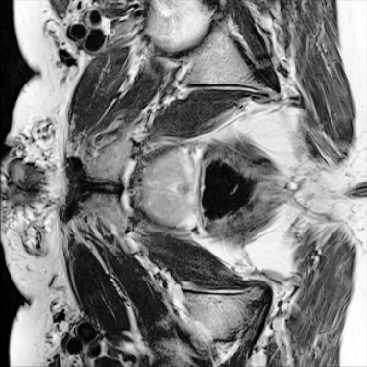
\includegraphics[width=\linewidth]{segmentation/segmentation_train_1.png}
		\caption{Obraz wejściowy}
		\label{fig:1}
	\end{subfigure}\hfil % <-- added
	\begin{subfigure}{0.25\textwidth}
		
\includegraphics[width=\linewidth]{segmentation/segmentaion_mask_1.png}
		\caption{Poprawna maska}
		\label{fig:2}
	\end{subfigure}\hfil % <-- added
	\begin{subfigure}{0.25\textwidth}
		
\includegraphics[width=\linewidth]{segmentation/pred_mask_1.png}
		\caption{Predykcja maski}
		\label{fig:3}
	\end{subfigure}
	
	\medskip
	\begin{subfigure}{0.25\textwidth}
		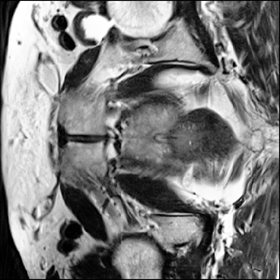
\includegraphics[width=\linewidth]{segmentation/segmentation_train_2.png}
		\caption{Obraz wejściowy}
		\label{fig:4}
	\end{subfigure}\hfil % <-- added
	\begin{subfigure}{0.25\textwidth}
		
\includegraphics[width=\linewidth]{segmentation/pred_mask_2.png}
		\caption{Poprawna maska}
		\label{fig:5}
	\end{subfigure}\hfil % <-- added
	\begin{subfigure}{0.25\textwidth}
		
\includegraphics[width=\linewidth]{segmentation/segmentation_mask_2.png}
		\caption{Predykcja maski}
		\label{fig:6}
	\end{subfigure}
	\caption{Przykłady wyników}
	\label{fig:images}
\end{figure}

\subsection{Alternatywne podejścia}
\begin{enumerate}
\item Rozszerzecznie zbioru treningowego poprzez augmentację danych zawierających obrazy przetworzone filtrem Gaussowskim powinno poprawić przypadki w których zdjęcie jest rozmyte.
\item Zwiększenie rozdzielczości obrazów wejściowych również powinno polepszyć wyniki segmentacji.
\end{enumerate}
Każde z wyżej opisanych podejść jest warte rozważenia, jednak z uwagi na stopień skomplikowania nie podjęliśmy się badaniu ich w pracy inżynierskiej.


\section{Moduł obliczania objętości}

Jedynym z celów pracy było zaproponowanie alternatywnej metody do liczenia objętości. Obecnie w szpitalu objętość gruczoły obliczana jest za pomocą aproksymacji przedstawionej wzorem:

\[V = (h_{max} - h_{min}) * S_{max} * 0.54\]
\\
gdzie 
\\
\(h_{max}\) - wysokość górnego końca gruczoły prostaty                     
\\
\(h_{min}\) - wysokość dolnego końca gruczoły prostaty                     
\\
\(S_{max}\) - pole powierzchni warstwy o największym, każdym liczonym jako:  

\[S_d = (i_{d_{max}} - i_{d_{min}}) * (j_{d_{max}} - j_{d_{min}})\] 

gdzie \\
\(i_{d_{max}}\) - pozycja najdalej wysuniętego pixela prostaty poziomo \\
\(i_{d_{min}}\) - pozycja najmniej wysuniętego pixela prostaty poziomo \\
\(j_{d_{max}}\) - pozycja najdalej wysuniętego pixela prostaty pionowo \\
\(j_{d_{min}}\) - pozycja najmniej wysuniętego pixela prostaty pionowo \\
d - indeks warstwy \\

Metoda polega na znalezieniu prostopadłościanu w który możemy wpisać gruczoł i obliczenie jego objętości. Następnie wartość jest przemnażana przez stałą aby przybliżyć kształt elipsoidą. Metoda wydaje się być niedokładna, co potwierdzają lekarze. Obecnie najdokładniejszą metodą jest zbadanie objętości po wycięciu gruczołu. Dowiedzieliśmy się, że wyniki uzyskane z aproksymacji objętości oraz wartości uzyskane po ekstrakcji są bardzo rozbieżne. 


Objętość voxela liczona jest wzorem:

\[ V_{d_{ij}} = PixelSpacing_0 * PixelSpacing_1 * SliceThickness\]
gdzie \\
\(PixelSpacing_0\) - pierwsza wartość atrybutu PixelSpacing (0028, 0030) z pliku DICOM \\
\(PixelSpacing_1\)  - druga wartość atrybutu PixelSpacing (0028, 0030) z pliku DICOM \\
\(SliceThickness\) - atrybut SliceThickness (0018, 0050) z pliku DICOM \\

Ze wzoru wynika, że wartości atrybutów nie wpływają na poprawność wyniku, stąd w dalszej części opisu dla uproszczenia przyjmiemy parametry pochodzące z pliku DICOM jako stałe równe 1. Przy współczynnikach jednostkowych wartość objętości warstwy jest równa polu powierzchni maski dla danej warstwy. Stąd w dalszej części będziemy posługiwać się polem powierzchni jako czynnikiem determinującym objętość.

\par
Postanowiliśmy zaproponować alternatywne rozwiązanie. Objętość w dalszych obliczeniach będziemy obliczać jako sumę voxeli znajdujących się w każdej z warstw obrazu. 

\[ V_{total} = \sum_{i=0}^{n} \sum_{d_i, j=0}^{m} V_{d_{ij}} \ gdzie\ d_{ij}\ pixelem\ maski \]
gdzie \\
n - liczba warstw pliku DICOM \\
m - liczba pixeli na warstwie \\

Aby zobrazować niedokładność aproksymacji elipsoidą postanowiliśmy porównać objętości za pomocą algorytmu aproksymującego oraz sumy objętości objętości kolejnych warstw voxeli na bazie masek określonych przez lekarzy. 

\begin{minipage}{\linewidth}
	\centering
	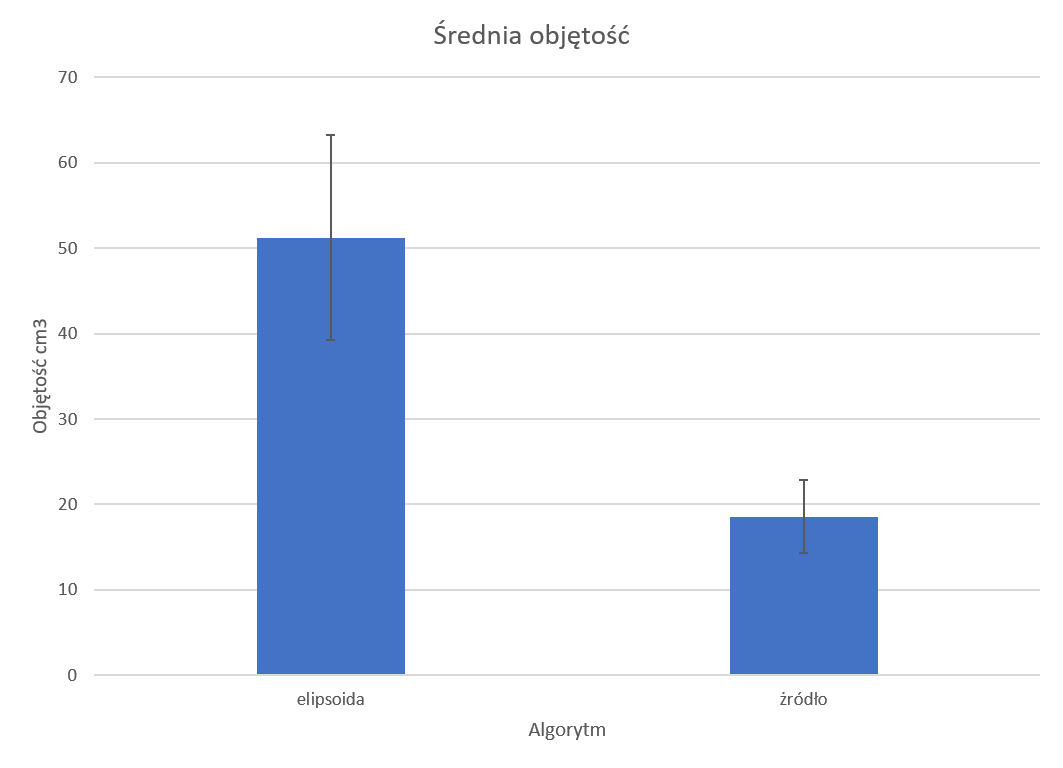
\includegraphics[width=\textwidth]{WstepObjetosc.png}
	\captionof{figure}{Średnia objętość uzyskana przy obliczaniu objętości przybliżając elipsoidą oraz przy sumowaniu voxeli}
\end{minipage}

Średnio różnica pomiędzy objętością obliczoną poprzez aproksymację elipsoidą daje wynik większy o 14954 (około 15 punktowy wynik w skali procentowej względem sumy objętości voxeli) dla tych samych masek. Ponieważ nie wykorzystujemy masek wyznaczonych przez lekarza tylko bazujemy na algorytmie segmentacji wymaga to dostosowania algorytmu do potrzeb tej pracy. W dalszej części przyjmiemy objętość wyznaczoną sumą jako wartość źródłową i będziemy oznaczać jako \textit{źródło}.

\subsection{Liczenie objętości}

Po pierwsze proponujemy aby wszystkie obrazy nie były traktowane jako całość, a objętość całej prostaty jest liczona metodą przekrojów jako objętość kolejnych warstw nachodzących po sobie, a końcowa objętość jest suma objętości. 

\[V = \sum_{i=0}^{n-1} ((S_i + S_{i+1}) * (h_{d_{i+1}} - h_{d_i})) / 2 \]
\\
gdzie\\
n - liczba warstw \\
\(d_i\) - indeksy kolejnych warstw obrazu \\
\(S_i\) - objętość kolejnych warstw obrazu \\
\(h_{d_i}\) - lokalizacja warstwy o indeksie \(d_{i}\) \\

Liczenie pola powierzchni maski została opisana w kolejnej sekcji. \\
W przypadku naszego systemu algorytm należy poprawić o niedokładność segmentacji prostaty. Zdarzają się sytuacje gdzie kolejna warstwa nie jest warstwą ostatnią na której znajduje się prostata a algorytm nie znalazł na zdjęciu prostaty. W tym przypadku bierzemy kolejną następującą po niej niepustą warstwę.

\subsection{Liczenie pola powierzchni}
Z uwagi na niedokładności masek zwracanych przez algorytm segmentacji proponujemy 3 alternatywne funkcje poprawiające obraz:
\begin{enumerate}
\item Pole powierzchni prostokąta na którym można opisać maskę. Najprostszy algorytm, wzorujący się bezpośrednio na obecnym podejściu stosowanym w szpitalu. Jednak w tym przypadku każdą warstwę opisujemy innym prostokątem, przez co wyniki powinny być dokładniejsze
\item Znalezienie otoczki wypukłej największego spójnego fragmentu maski. Alternatywnym podejściem do rozwiązania problemu jest algorytm znajdujący otoczkę wypukła dla największego spójnego elementu. Jest rozwiązaniem gdzie wyszukujemy kształt o największym polu powierzchni, a następnie liczymy tylko jego pole pomijając miejsca gdzie również została znaleziona prostata. W tym przypadku pole powierzchni jest policzone dużo dokładniej, niż w pierwszym przypadku jednak gdy maska nie jest spójna mogą być mocno zaniżone. 
\item Znalezienie otoczki wypukłej dla wszystkich elementów maski. Jest to modyfikacja poprzedniego algorytmu , w której szukamy otoczki wypukłej dla wszystkich pixeli maski.
\end{enumerate}

Następnie pole powierzchni liczone jest jako pole poligonu uzyskanego w procesie poprawiania obrazu. Poniżej przedstawiamy różnice wynikające z zastosowania każdego z algorytmów.

Przykład pierwszy, w którym wysegmentowana maska jest jednym spójnym elementem. \\ \\


\begin{figure}[htb]
	\centering % <-- added
	\begin{subfigure}{0.25\textwidth}
		
\includegraphics[width=\linewidth]{Mask/1/maska.png}
		\caption{Maska przykład 1}
		\label{fig:1}
	\end{subfigure}\hfil % <-- added
	\begin{subfigure}{0.25\textwidth}
		
\includegraphics[width=\linewidth]{Mask/1/square.png}
		\caption{Maska przykład 1 Wpisana w prostokąt}
		\label{fig:2}
	\end{subfigure}\hfil % <-- added
	
	\medskip
	\begin{subfigure}{0.25\textwidth}
		
\includegraphics[width=\linewidth]{Mask/1/hull.png}
		\caption{Maska przykład 1 Otoczka wokół największego elementu}
		\label{fig:3}
	\end{subfigure}\hfil % <-- added
	\begin{subfigure}{0.25\textwidth}
		
\includegraphics[width=\linewidth]{Mask/1/hull.png}
		\caption{Maska przykład 1 Otoczka wypukła}
		\label{fig:4}
	\end{subfigure}\hfil % <-- added

	\caption{Przykłady wyników}
	\label{fig:images}
\end{figure}


Algorytmy liczenia otoczek wypukłych dają ten sam rezultat w przypadku gdy maska jest spójna. Przykład obrazuje naddatek jaki pojawia się przy aproksymowaniu maski prostokątem. Prostata jest kształtem, który nie odpowiada, żadnemu kształtowi geometrycznemu, stąd przybliżanie go czworokątem jest nieefektywne.

Przykład drugi, w którym wysegmentowana maska nie jest spójna. \\ \\

\begin{figure}[htb]
	\centering % <-- added
	\begin{subfigure}{0.25\textwidth}
		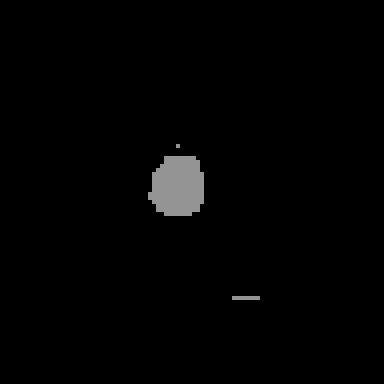
\includegraphics[width=\linewidth]{Mask/2/mask.png}
		\caption{Maska przykład 2}
		\label{fig:1}
	\end{subfigure}\hfil % <-- added
	\begin{subfigure}{0.25\textwidth}
		
\includegraphics[width=\linewidth]{Mask/2/square.png}
		\caption{Maska przykład 2 Wpisana w prostokąt}
		\label{fig:2}
	\end{subfigure}\hfil % <-- added
	
	\medskip
	\begin{subfigure}{0.25\textwidth}
		
\includegraphics[width=\linewidth]{Mask/2/biggest.png}
		\caption{Maska przykład 2 Otoczka wokół największego elementu}
		\label{fig:3}
	\end{subfigure}\hfil % <-- added
	\begin{subfigure}{0.25\textwidth}
		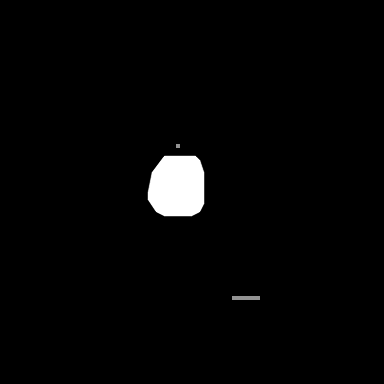
\includegraphics[width=\linewidth]{Mask/2/hull.png}
		\caption{Maska przykład 2 Otoczka wypukła}
		\label{fig:4}
	\end{subfigure}\hfil % <-- added
	
	\caption{Przykłady wyników}
	\label{fig:images}
\end{figure}

Widać dużą różnicę między algorytmami liczenia otoczek wypukłych. Ponieważ prostata jest znaleziona częściowo w kilku elementach obrazu, algorytm liczący otoczkę dla całości obrazu daje o wiele większy wynik niż liczący tylko dla największego spójnego fragmentu. Przykład obrazuje jak ważną rolę pełni algorytm segmentacji w procesie liczenia objętości.

\subsection{Analiza wyników}
Aby przeanalizować wyniki osiągnięte przez proponowany przez nas algorytm segmentacji oraz liczenia objętości postanowiliśmy porównać wyniki liczenia objętości algorytmem szpitalnym na danych konkursowych (segmentacja prostaty została wykonana przez lekarza) oraz proponowane przez nas metody liczenia objętości na maskach uzyskanych w przez aplikacyjny system segmentacji wraz z metodami poprawy obrazu. Zbiór testowy składał się z 13 pacjentów pochodzących z danych konkursowych. Wartości uzyskane dla każdego z nich, oraz różnice pomiędzy wynikiem oraz wartością źródłową przedstawia tabela \ref{Objętości pacjenci}.

\begin{table}[h!]
\caption{Wartości objętości}
\centering
\begin{tabular}{|l|c|c|c|c|c|} \hline  
Pacjent             & Źródło	&  Otoczka element	 & Wpisanie w kwadrat	& Otoczka cała          \\ \hline
Prostate3T-01-0001	& 47960,50	& 21678,25(26282,25) & 	28081(19879,5)	    & 23481,5(24479)        \\ \hline
Prostate3T-01-0006	& 58901,50	& 49371,75(9529,75)	 & 68668(-9766,5)	    & 55471,75(3429,75)     \\ \hline
Prostate3T-01-0007	& 24694,75	& 9917,75(14777)	 & 24806,5(-111,75)	    & 18679,75(6015)        \\ \hline
Prostate3T-01-0008	& 48364,75	& 27709,5(20655,25)	 & 44875(3489,75)	    & 34201,75(14163)       \\ \hline
Prostate3T-01-0009	& 129628,75	& 81372,25(48256,5)	 & 107769(21859,75)	    & 86835,75(42793)       \\ \hline
ProstateDx-02-0002	& 141604,50	& 89050,5(52554)	 & 638992(-497387,5)	& 248745,5(-107141)     \\ \hline
ProstateDx-02-0003	& 185655,25	& 145749(39906,25)	 & 221833(-36177,75)	& 168329,25(17326)      \\ \hline
ProstateDx-02-0004	& 176572,00	& 91919,25(84652,75) & 	162448,5(14123,5)	& 116387,75(60184,25)   \\ \hline
ProstateDx-02-0005	& 117470,00	& 50078(67392)	     & 7532 1(42149)	    & 59246,75(58223,25)    \\ \hline
ProstateDx-03-0002	& 67898,75	& 98652(-30753,25)	 & 137690(-69791,25)	& 111755(-43856,25)     \\ \hline
ProstateDx-03-0003	& 133893,00	& 66159,75(67733,25) & 	147515,5(-13622,5)	& 109883(24010)         \\ \hline
ProstateDx-03-0004	& 81947,50	& 124994,5(-43047)	 & 265676(-183728,5)	& 192162,75(-110215,25) \\ \hline
ProstateDx-03-0005	& 125858,25	& 113662,5(12195,75) & 	172718,5(-46860,25)	& 137877,5(-12019,25)   \\ \hline 
\end{tabular}
\label{Objętości pacjenci}
\end{table}

Rozbieżność pomiędzy wynikami przeprowadzonymi na maskach uzyskanych poprzez segmentację przez lekarza i przez algorytm różnią się znacząco. 
\par
Największym problemem jaki zaobserwowaliśmy jest w przypadku gdy maska zostanie wykryta przez algorytm na warstwie, która znajduje się dużo przed faktycznym początkiem prostaty. Najbardziej jest to widoczne na przykładzie pacjenta \textit{ProstateDx-02-0002}, dla którego wyniki uzyskany przez nasz algorytm są nawet dwukrotnie większe. Prostata znajduje się między 9 a 18 warstwą, jednak algorytm segmentacji wykrył obecność prostaty już na warstwie 4. 
\par 
Dla przypadków, w których maski są znalezione na tych samych warstwach (to znaczy początek i koniec na obrazach o tym samym indeksie w przypadku danych konkursowych oraz algorytmu segmentacji), jak na przykład \textit{Prostate3T-01-0007} uzyskujemy wyniki zbliżone do wartości źródłowej. Błąd tutaj wynika z niedokładności algorytmu segmentacji.
 

\begin{minipage}{\linewidth}
	\centering
	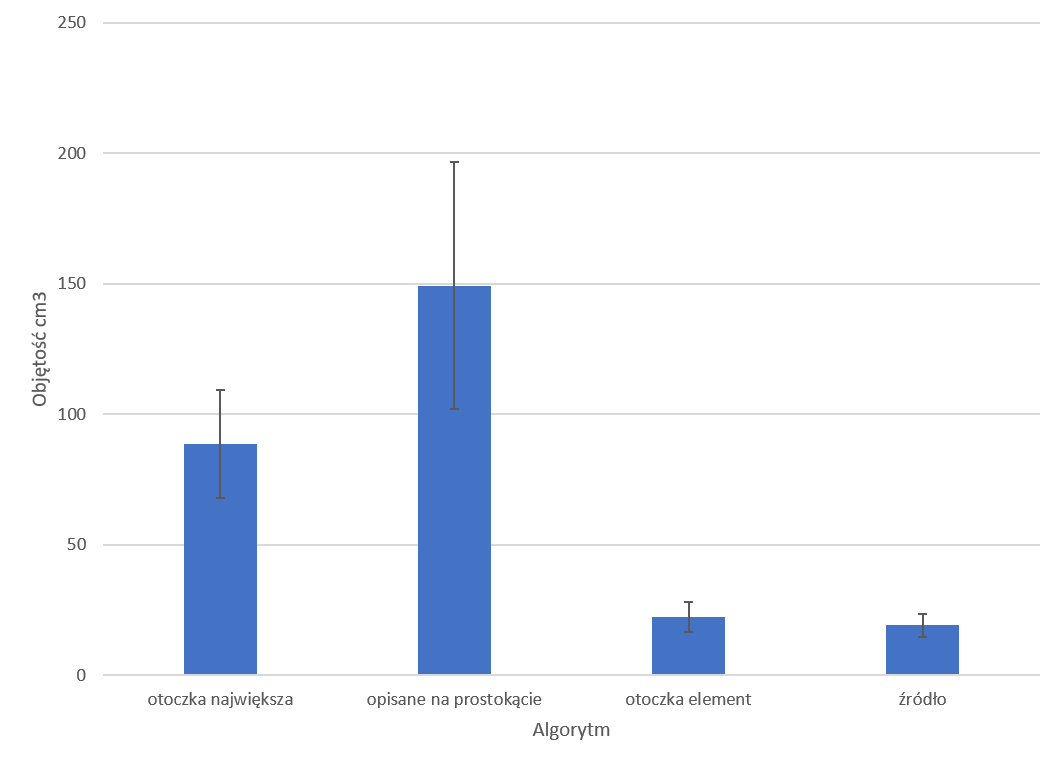
\includegraphics[width=\textwidth]{WynikiObjetosc.png}
	\captionof{figure}{Porównanie metod liczenia}
\end{minipage}

Tabela \ref{Analiza statystyczna algorytmów} przedstawia statystyki porównujące opisywane algorytmy z danymi źródłowymi. Jak widać najlepszą metodą przybliżenia jest otoczka wypukła wokół wszystkich elementów maski. Nie występuje w nim niedoszacowanie, które można zaobserwować w algorytmie znajdującym otoczę tylko wokół największego kształtu maski. Algorytm aproksymujący kształt maski prostokątem następnie sumujący voxele na każdej warstwie okazał się rozwiązaniem wysoce nieskutecznym z uwagi na duże przeszacowanie. Algorytm daje złe wyniki w szczególności gdy maska nie jest spójna. Wówczas występuje duże przeszacowanie.

\begin{table}[h!]
\caption{Analiza statystyczna algorytmów}
\centering
\begin{tabular}{|l|c|c|c|c|} \hline  
Algorytm & Różnice średniej (\%) & Różnice odchylenie (\%) & Min & Max \\ \hline 
Otoczka element	       & 28\%	            & 19\%	                & 9917,75	          &   145749           \\ \hline
Wpisanie w kwadrat	   & -56\%	            & -213\%	                & 24806,5	          &   638992           \\ \hline
Otoczka cała	       & -2\%	            & -34\%	                & 18679,75	          &   248745,5         \\ \hline
\end{tabular}
\label{Analiza statystyczna algorytmów}
\end{table}

Z zaproponowanych algorytmów jedynym który osiągnął większa dokładność niż algorytm aproksymujący elipsoidą jest algorytm znajdujący otoczkę wypukłą dla całej maski. Pierwszy miał około 15 procentowe przeszacowania, natomiast drugi około 2\% niedoszacowanie względem danych źródłowych. Pokazuje to, że istnieją lepsze algorytmy niż obecnie najczęściej stosowany.

\subsection{Alternatywne podejścia}
Algorytmy opisane powyżej są jednymi z wielu możliwości poprawienia efektywności badania objętości prostaty w sposób analityczny. Jak widać w dużej mierze objętość opiera się o dokładność segmentacji. Wartymi do rozważenia modyfikacjami jest również
\begin{description}
\item Pole powierzchni prostokąta na którym można opisać największy spójny element uzyskany w procesie segmentacji. Z uwagi na małe zróżnicowanie względem opisanych przez nas metod nie uwzględniliśmy jej w algorytmach udostępnianych przez naszą aplikację
\item Wybór elementów wokół których szukamy otoczki wypukłej na podstawie pewnej funkcji. Jest to zagadnienie skomplikowane, ponieważ możliwych funkcji jest bardzo dużo. Na przykład moglibyśmy szukać otoczki wokół wszystkich elementów maski znajdujących się w określonej odległości od środka największego elementu maski.
\item Przy poprawianiu maski uwzględniamy wszystkie warstwy. Czyli w przypadku gdy aktualna maska jest niespójna z poprzedzającą oraz następującą po sobie, wówczas zamiast niej bierzemy maskę będącą średnią dwóch wymienionych.
\end{description}

\section{Moduł backedowy}

Moduł zaimplementowany w .NET Framework odpowiada za komunikację z warstwą prezentacji, komunikację między resztą serwisów oraz dostępem do bazy danych. Podstawowe funkcje
\begin{enumerate}
\item Udostępnia API do komunikacji z naszym modułem frontendowym oraz umożliwiający integrację z dowolnym innym systemem, który mógłby wykorzystywać nasze API. Interfejs zapewnia pełen dostęp do tabel czyli wszystkie operacje \textit{CRUD} jakie mogą być potrzebne przy rozwoju systemu. Dodatkowo daje zapewnia komunikację użytkownika ze wszystkimi kontenerami. W tym przypadku zakres operacji jest ograniczony do minimum.
\item Obsługę bazy danych. W tym obsługę dodawania nowych pacjentów z plików oraz systemu PACS, migrację bazy danych oraz obsługę kwerend i procedur.
\item Komunikację z pozostałymi komponentami backendowymi.
\end{enumerate}

Staraliśmy się w pracy zastosować wszystkie najlepsze praktyki wykorzystywane przy projektowaniu oprogramowania takie jak zasady \textit{SOLID} oraz wzorce projektowe jak \textit{Dependency Injection}. Za spełnienie tego ostatniego w aplikacji odpowiada kontener Autofac.

\subsection{Diagram zależności}
\begin{minipage}{\linewidth}
	\centering
	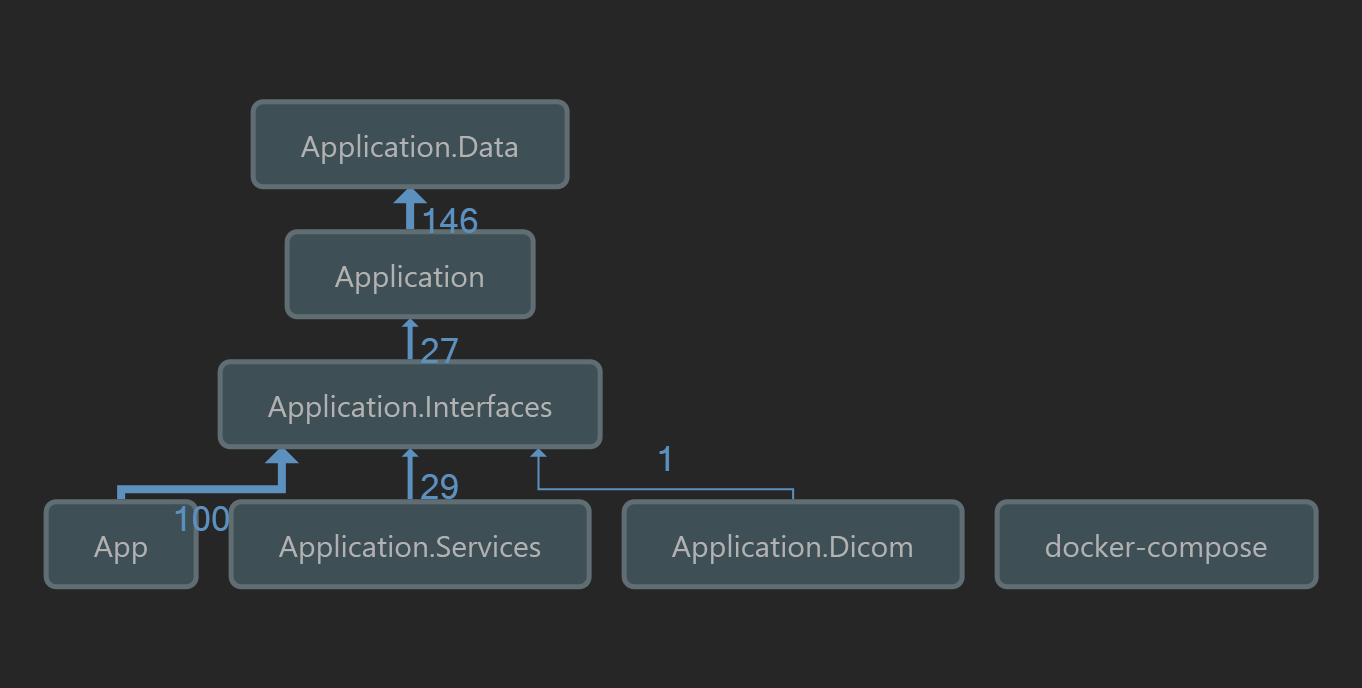
\includegraphics[width=\textwidth]{Backend/ApplicationDependencies.png}
	\captionof{figure}{Diagram zależności}
\end{minipage}

Jak widać podstawowe projekty w systemie to
\begin{enumerate}
\item Application.Data - który jest warstwą dostępu do danych w aplikacji, definiuje encje oraz zarządza połączeniem z bazą danych.
\item Application - definiuje podstawowe obiektu współdzielone między modułami takie jak modele, wyjątki, logowanie, mapowanie obiektów.
\item Applicaition.Interfaces - projekt definiuje wszystkie kontrakty za pomocą których klasy komunikują się ze sobą
\item Applicaition.Services - zawiera implementację interfejsów zdefiniowanych w projekcie \textit{Interfaces}.
\item Application.Dicom - odpowiada za obsługę plików DICOM. Moglibyśmy zaimplementować go w projekcie \textit{Services} jednak z uwagi na złożoność zdecydowaliśmy umieści go w osobnym module.
\end{enumerate}

Projektując architekturę rozwiązania zależało nam aby komponenty były ze sobą luźno powiązane, przez co unikniemy niepotrzebnych nad którymi trudno zapanować. Moduły podstawowe są zależne tylko do projektu \textit{Interfaces} co zapewnia oczekiwane luźne łączenie i komunikację pomiędzy nimi. Warto zauważyć, że projekt który udostępnia nasze REST API jest zależny tylko od projektu \textit{Interfaces}.

\subsection{Baza danych}

Plik wejściowy jest plikiem binarnym zawierającym wiele informacji o pacjencie, w przypadku aplikacji, którą tworzymy przy każdym odwołaniu do kolejnych warstw przetwarzanie pliku jest bardzo nieefektywne. Dlatego postanowiliśmy plik przetwarzać tylko raz przy dodawaniu, a przy odwołaniach zwracać dane z bazy danych.
\par
Ponieważ według standardu DICOM \cite{standardDICOM} zawiera ponad 4 tysiące tagów. Po przeanalizowaniu plików wejściowych zauważyliśmy, że w naszym przypadku uzupełniona jest tylko część danych. 
\par
W bazie danych przechowujemy wybrane dane istotne z punktu widzenia działania aplikacji oraz potrzeb lekarza. Wybraliśmy strukturę gdzie dla jednego pacjenta informację na temat obrazów oraz danych są wspólne i nie zmieniają się dla kolejnych warstw obrazu. Dlatego jedyne informacje dotyczące obrazu są przechowywane dla każdego pliku osobno. Poniżej zamieszczono diagram encji jakie znajdują się w bazie danych.

\begin{minipage}{\linewidth}
	\centering
	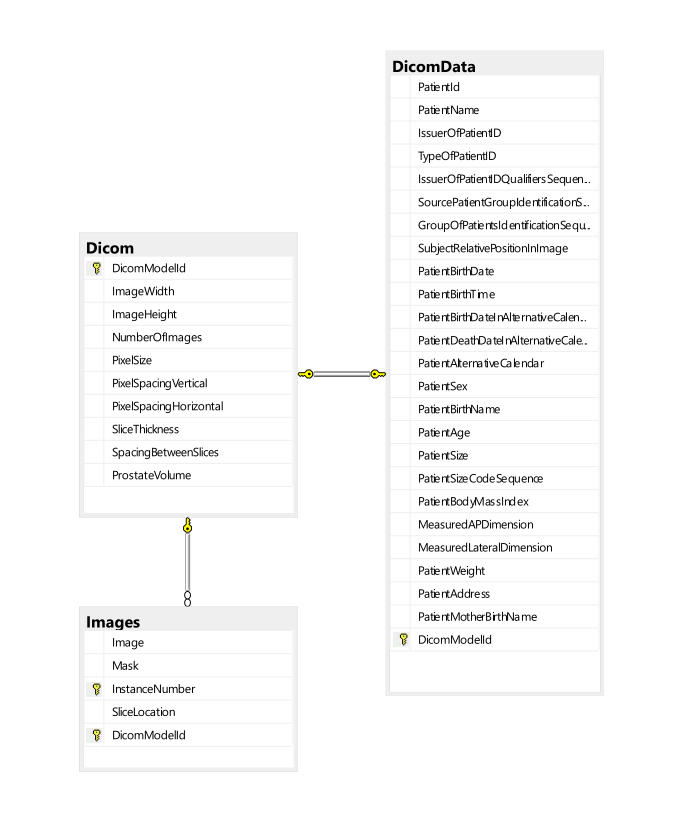
\includegraphics[width=\textwidth]{Backend/SchematBazy.png}
	\captionof{figure}{Schemat bazy danych}
\end{minipage}

\section{Moduł prezentacji}
Aplikacja jest stworzona w architekturze SPA (Single Page Application). Wykorzystanie tego podejścia pozwala na wyświetlanie wielu widoków bez konieczności pobierania ponownie tych samych informacji, dzięki temu zachowując płynne działanie strony internetowej. Stusując te podejście zyskujemy na płynności działania oraz lepsze odczucia użytkownika przy korzystaniu z serwisu.

Naszą aplikację stworzyliśmy przy pomocy biblioteki React. Ułatwia ona myślenie o logice biznesowej aplikacji dzieląc stronę na komponenty. Każdy komponent składa się z co najmniej jednego HTML tagu i jest odpowiedzialny za inną część widoczną na stronie. Granulacja komponentów sprzyja pisaniu złożonych aplikacji poprzez separację stanów każdego z komponentów.
Naszą aplikację stworzyliśmy przy pomocy biblioteki React. Ułatwia ona myślenie o logice biznesowej aplikacji dzieląc stronę na komponenty. Każdy komponent składa się z co najmniej jednego HTML tagu i jest odpowiedzialny za inną część widoczną na stronie. Granulacja komponentów sprzyja pisaniu złożonych aplikacji poprzez separację stanów każdego z komponentów.

\subsection{Widok startowy}
Pierwszy ekran jaki jest wyświetlany w naszej spełnia trzy podstawowe funkcjonalności.
\begin{enumerate}
\item Wyświetlenie listy pacjentów dostępnych w aplikacji.
\item Dodanie nowego użytkownika do bazy danych.
\item Integracja z systemem PACS.
\end{enumerate}

\begin{minipage}{\linewidth}
	\centering
	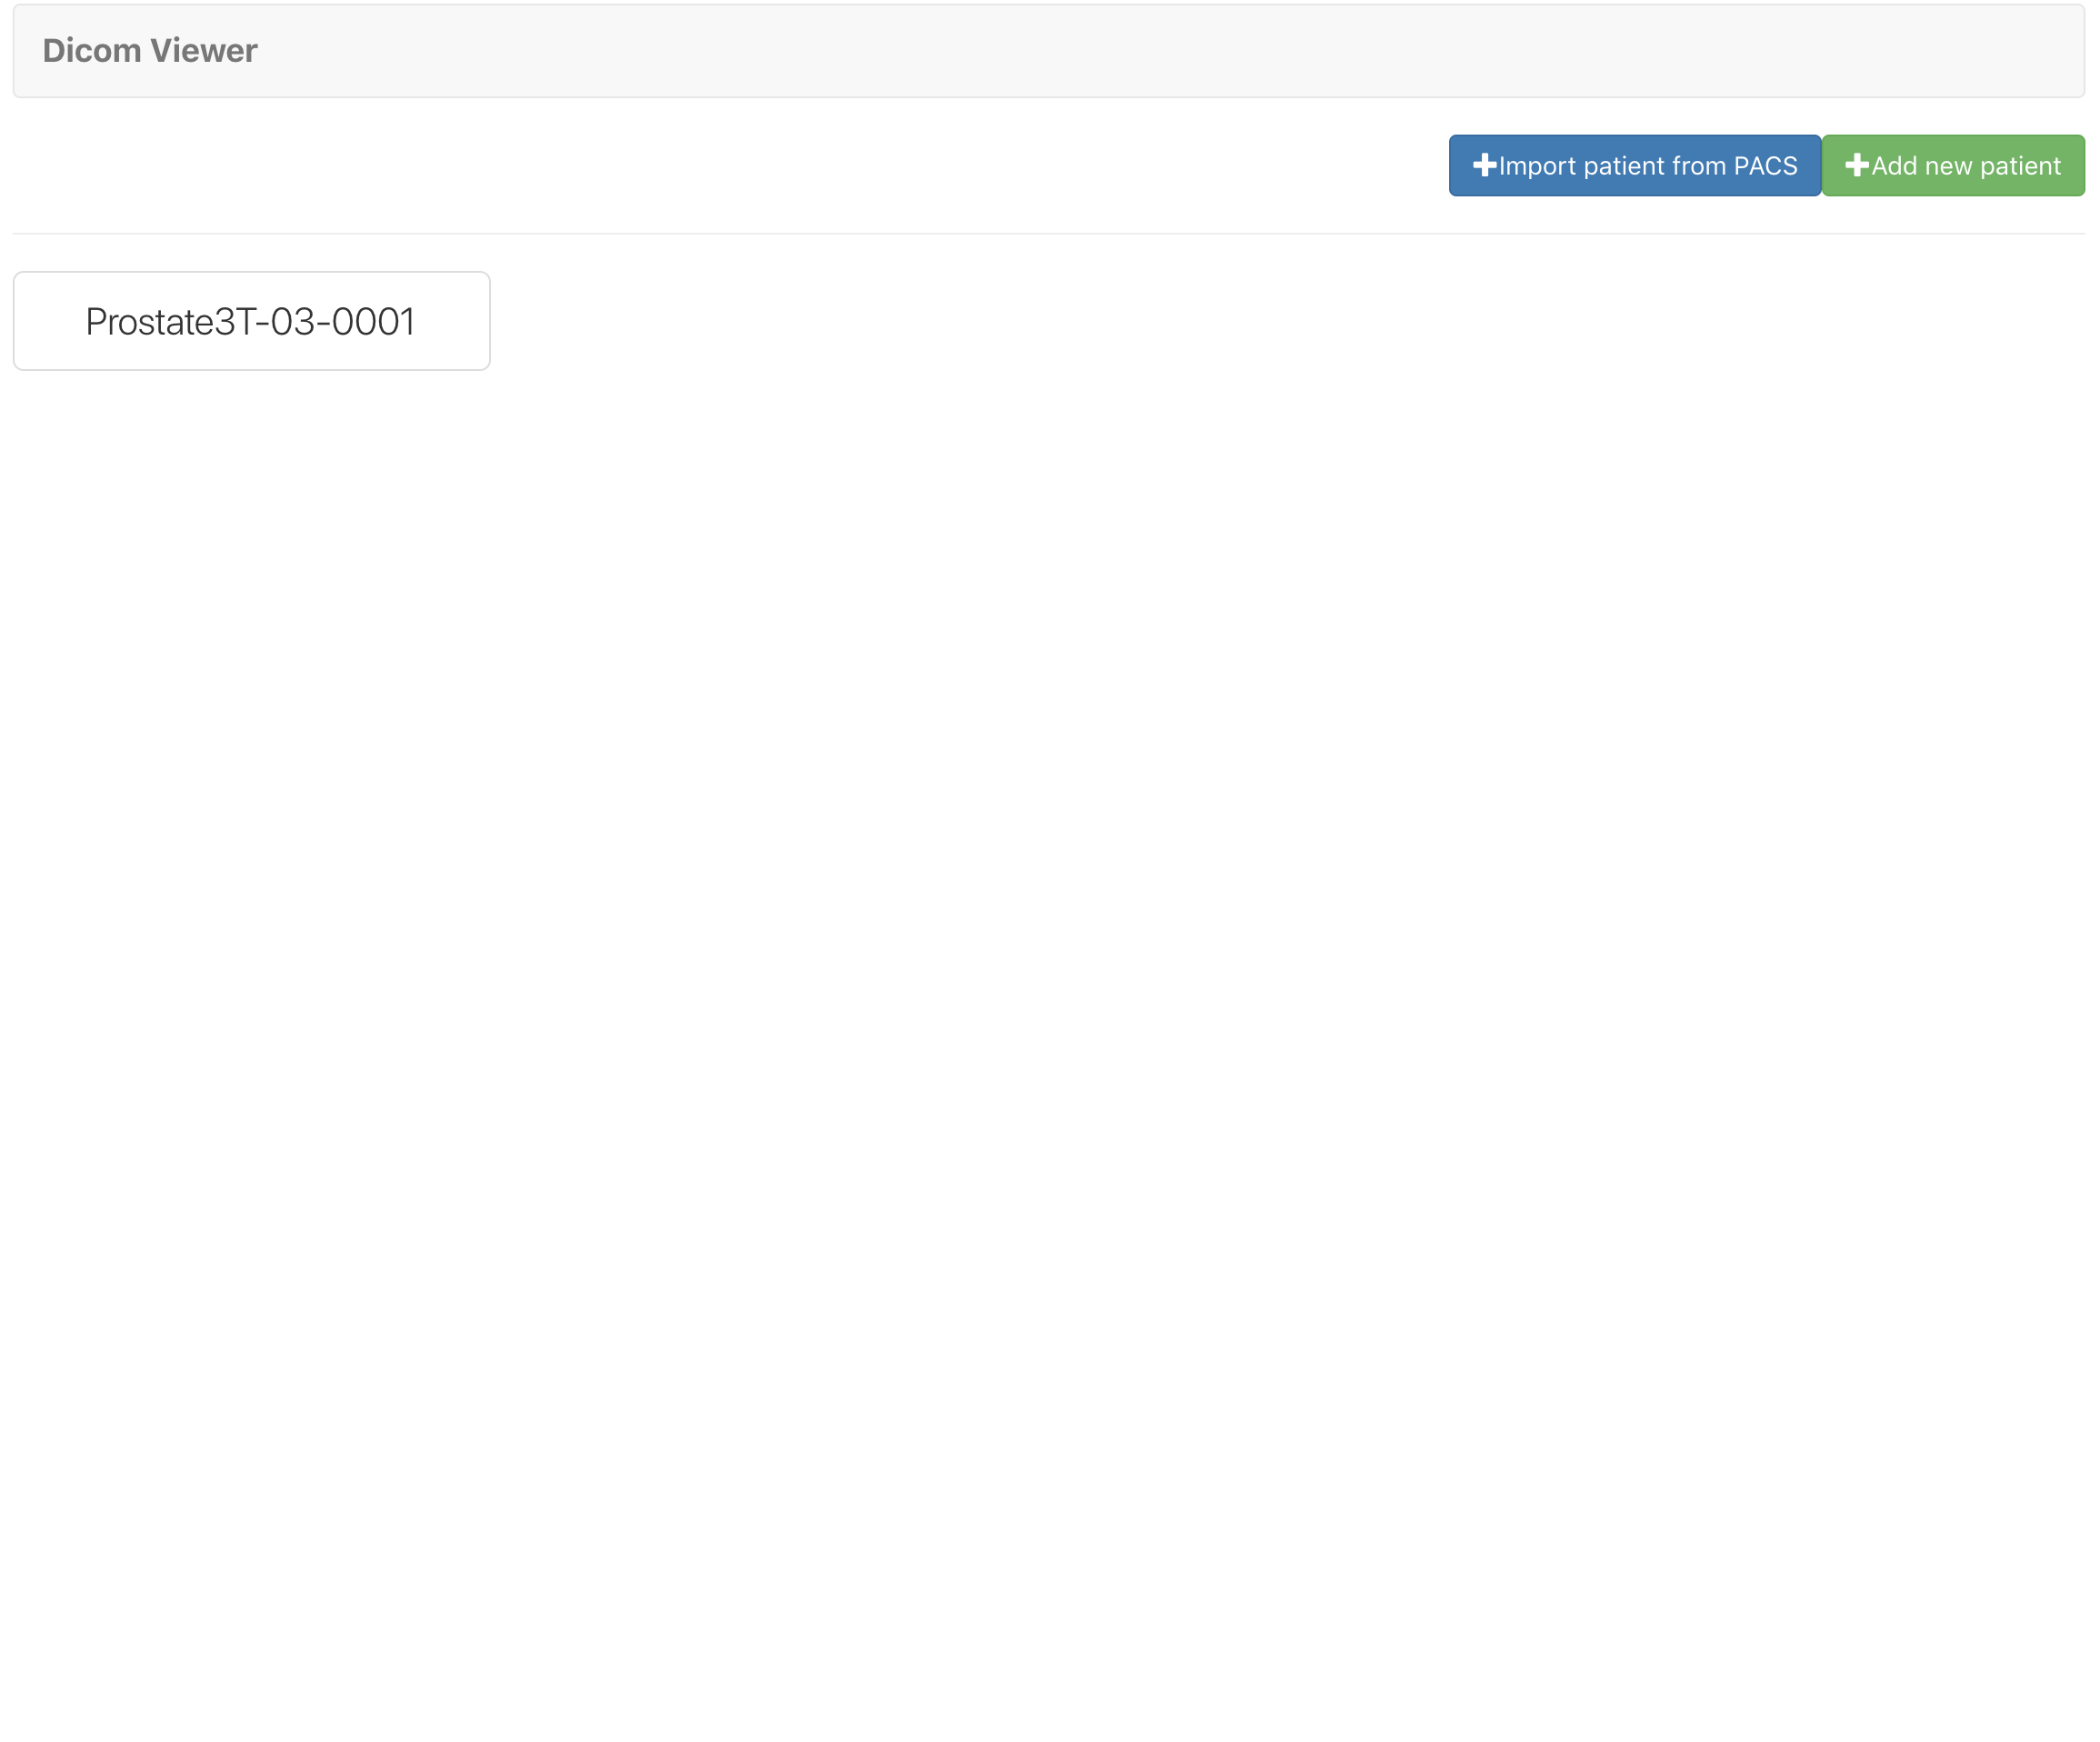
\includegraphics[width=0.5\textwidth]{FrontScreen/Main/0.png}
	\captionof{figure}{Ekran startowy}
\end{minipage}

Aby dodać nowego pacjenta, należy nacisnąć przycisk \textit{Add New Patient}.Pojawi się nowe okno w którym użytkownik powinien wybrać wszystkie pliki z danymi pacjenta, następnie nacisnąc \textit{Upload}. Po udanym procesie należy zamknąć okienko.
\par
Typowym scenariuszem jest dodawanie pacjenta wraz ze wszystkimi obrazami jakie mamy na jego temat. Pliki średnio ważą około 10 MB, w zależności od ilości wartstw obrazu oraz szybkości połączenia internetowego czasy dodawania mogą być wydłużone.
\begin{minipage}{\linewidth}
	\centering
	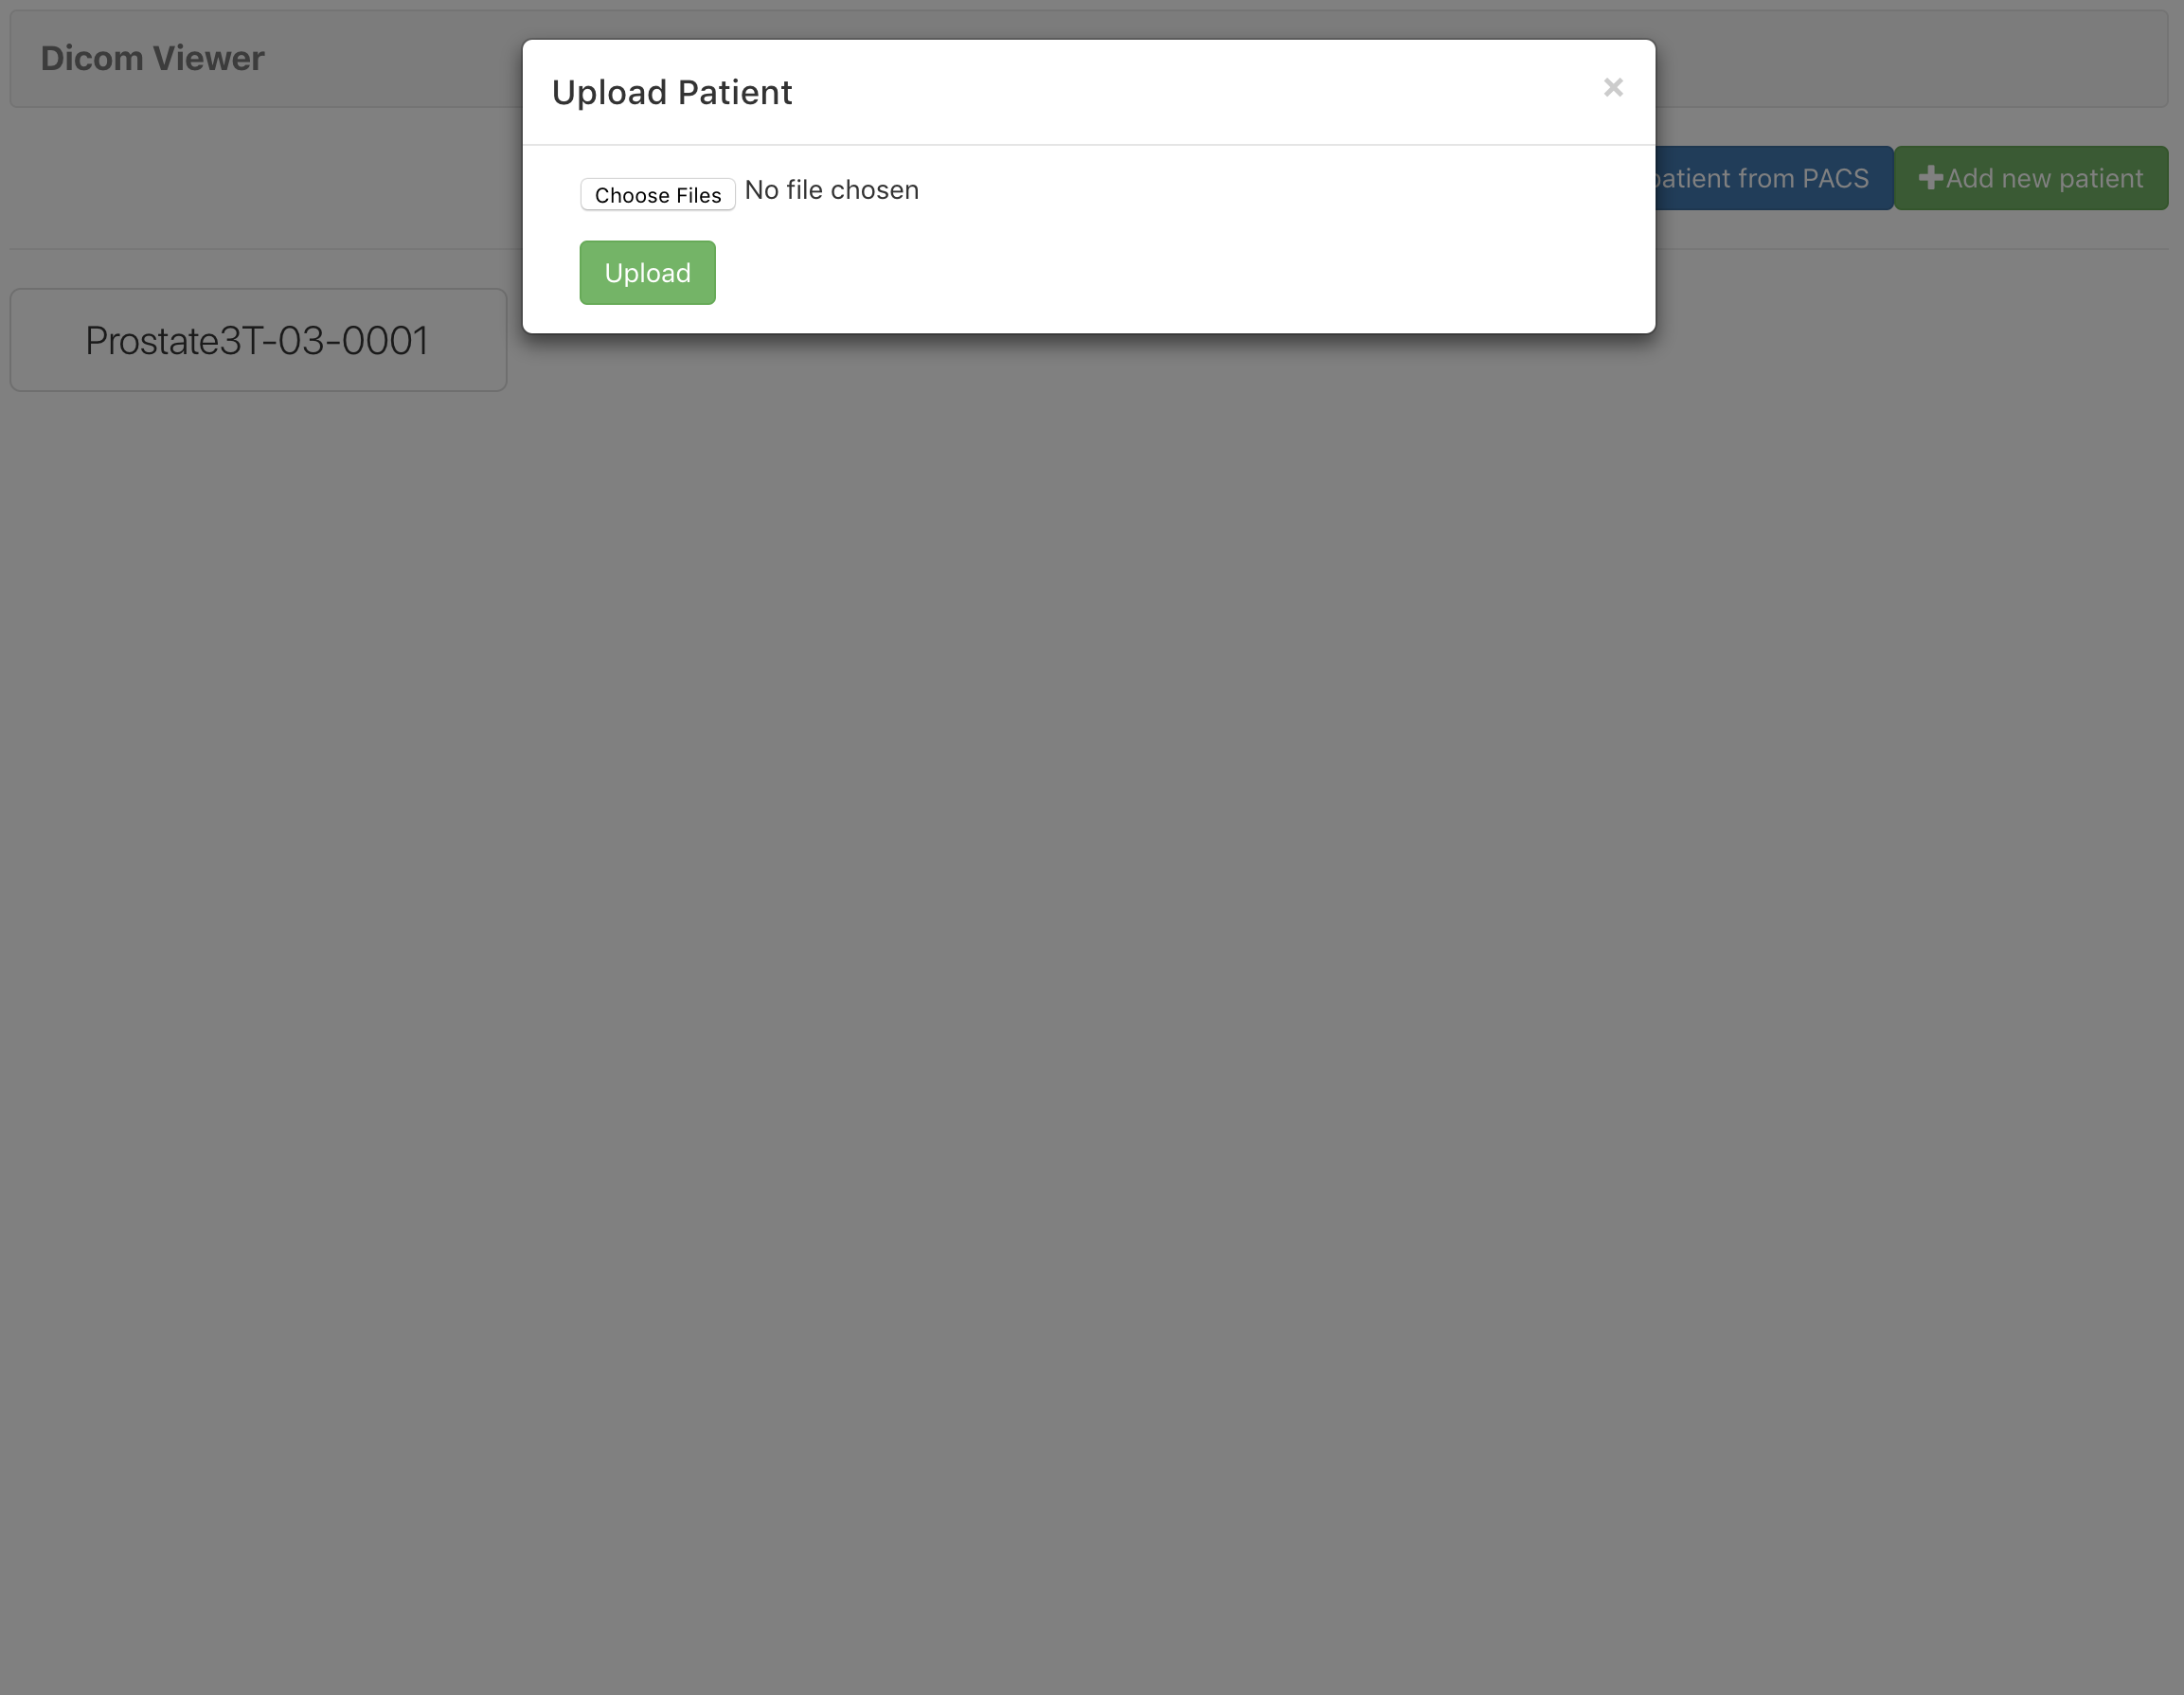
\includegraphics[width=0.5\textwidth]{FrontScreen/Main/15.png}
	\captionof{figure}{Dodawanie pacjenta}
\end{minipage}
\begin{minipage}{\linewidth}
	\centering
	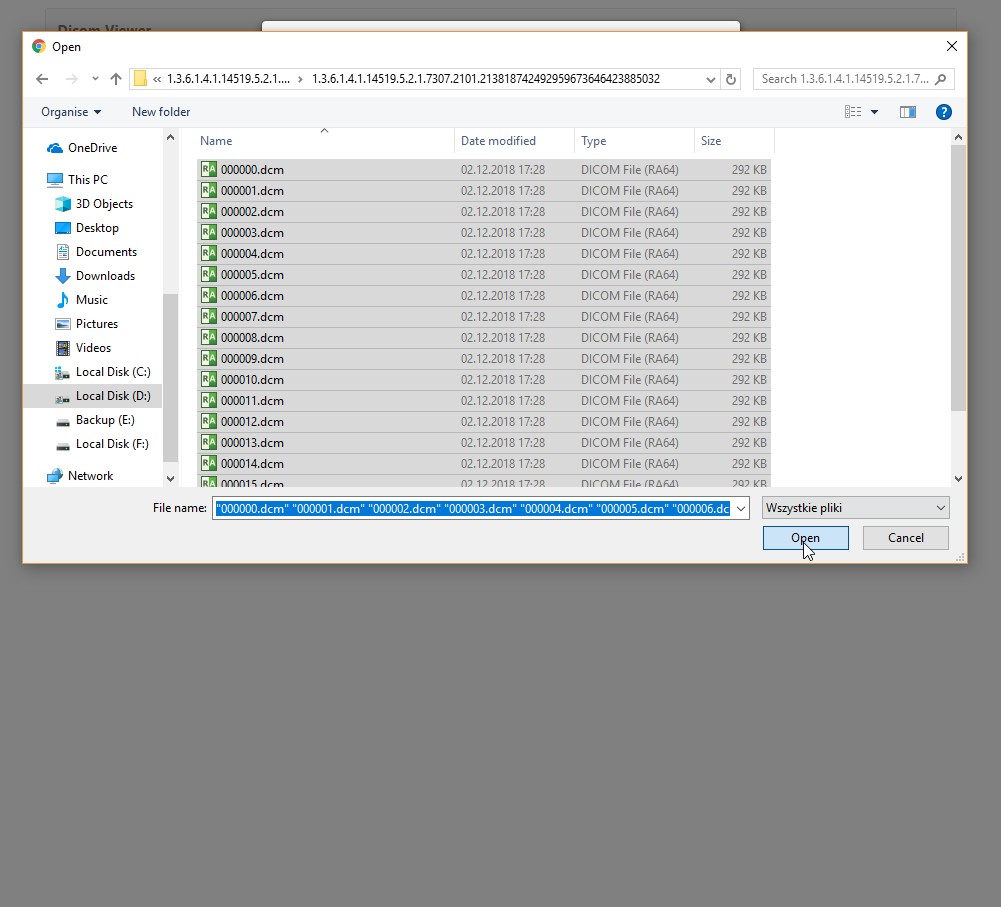
\includegraphics[width=0.5\textwidth]{FrontScreen/Main/95.png}
	\captionof{figure}{Wybór plików}
\end{minipage}
\begin{minipage}{\linewidth}
	\centering
	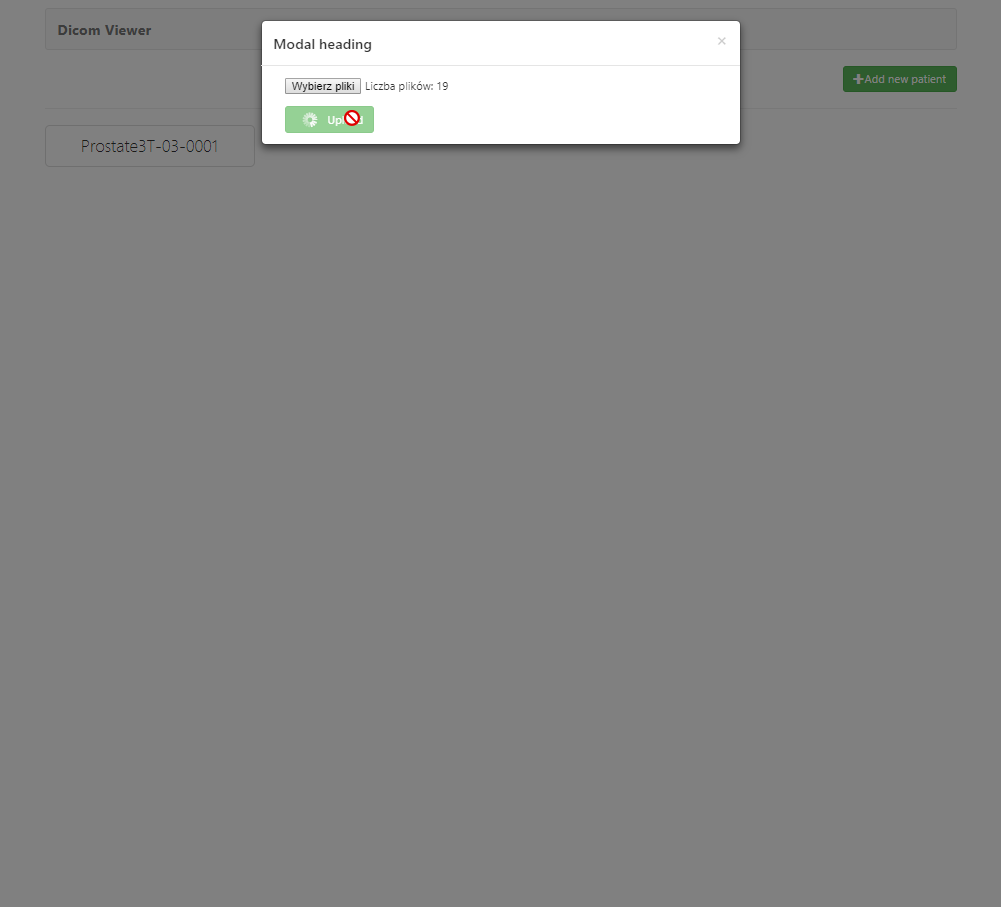
\includegraphics[width=0.5\textwidth]{FrontScreen/Main/114.png}
	\captionof{figure}{Proces zakończony}
\end{minipage}
\begin{minipage}{\linewidth}
	\centering
	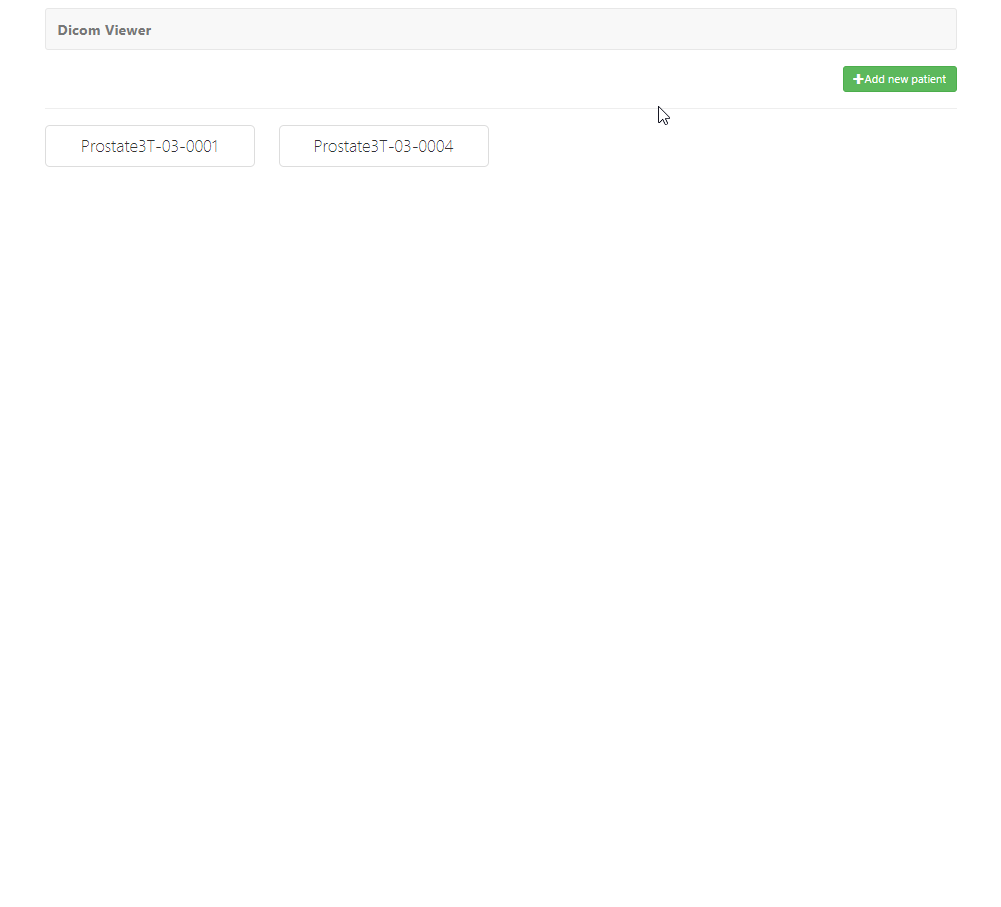
\includegraphics[width=0.5\textwidth]{FrontScreen/Main/410.png}
	\captionof{figure}{Proces zakończony}
\end{minipage}


\subsection{Widok pacjenta}

Lista pacjentów wyświetla ich identyfikatory w systemie. Aby przejść do widoku wyświetlającego wszystkie informacje o pacjencie należy nacisnąć na wybranego pacjenta.

\begin{minipage}{\linewidth}
	\centering
	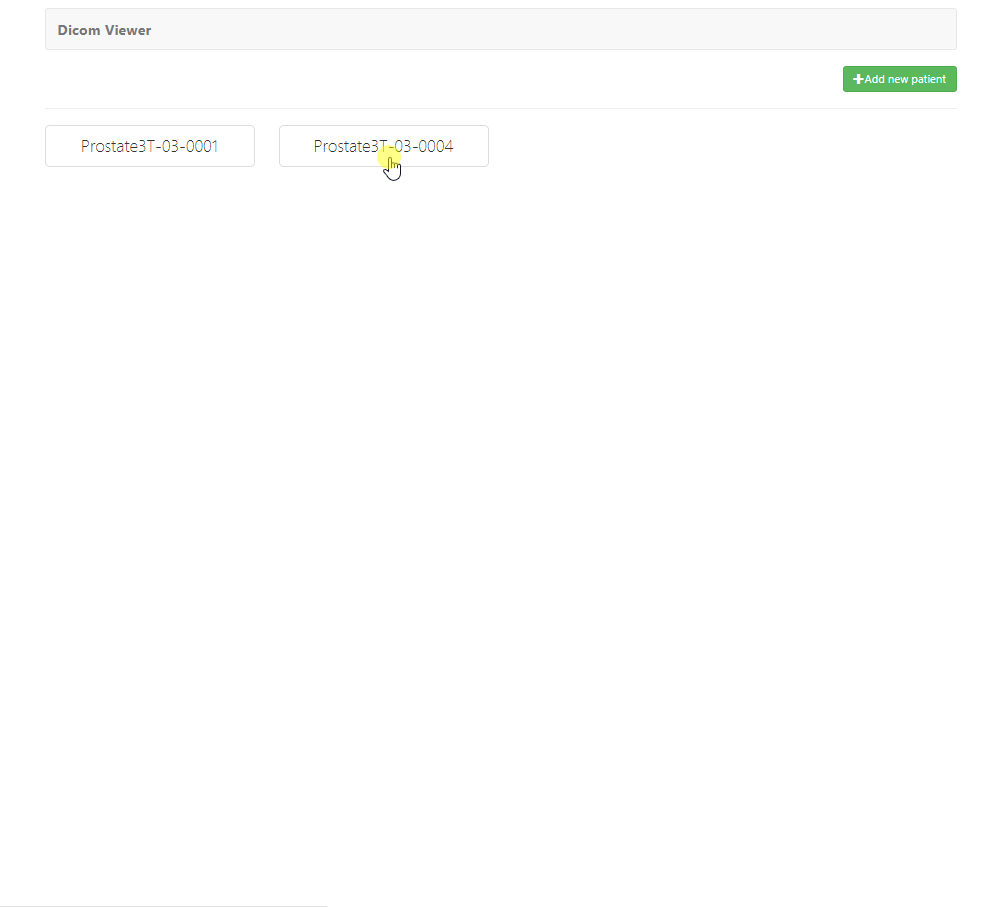
\includegraphics[width=0.5\textwidth]{FrontScreen/Patient/0.png}
	\captionof{figure}{Przejście do widoku pacjenta}
\end{minipage}

Widok pacjenta przedstawia nam wszystkie informacje jakie posiadamy na temat danego przypadku badanego. W szczególności:
\begin{description}
\item Dane pacjenta z pliku DICOM, takie jak: nazwa, wiek, płeć, wzrost, waga oraz inne. Wyświetlamy tylko informacje, które w danym pliku się znajdowały. Jeżeli jakieś dane miały wartość pustą pomijamy je. Jeżeli dane podlegały wcześniejszej anonimizacji dane wrażliwe jakie zobaczymy na interfejsie użytkownika nie będą danymi odpowiadającymi tym z systemu szpitalnego.
\item Informacje na temat obrazu, takie jak: wymiary obrazu (szerokość i wysokość), odległość między kolejnymi obrazami w badaniu, odległości między konkretnymi pixelami na obrazie.
\item Informacje na temat objętości oraz przyciski do kalkulacji objętości według wybranego algorytmu.
\item Obraz z rezonansu magnetycznego oraz maskę znalezioną w procesie segmentacji wraz z możliwością edycji.
\end{description}

\begin{minipage}{\linewidth}
	\centering
	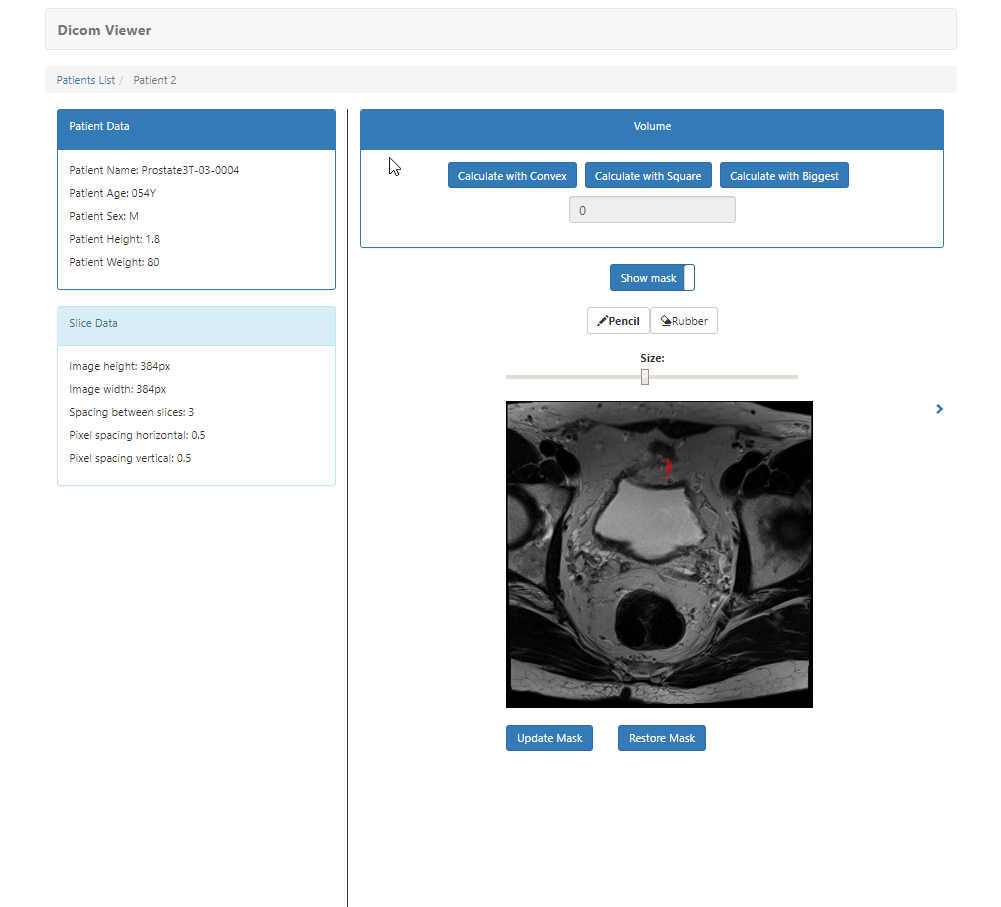
\includegraphics[width=0.5\textwidth]{FrontScreen/Patient/22.png}
	\captionof{figure}{Widok pacjenta}
\end{minipage}

Aby obliczyć objętość na podstawie masek znajdujących się obecnie w bazie danych należy nacisnąć odpowiedni przycisk znajdujący się na górze strony. Udostępniamy trzy alternatywne metody opisane w poprzednim rozdziale. Po naciśnięciu przycisku objętość jest obliczana oraz automatycznie aktualizowana na stronie tak jak i w bazie danych.

\begin{minipage}{\linewidth}
	\centering
	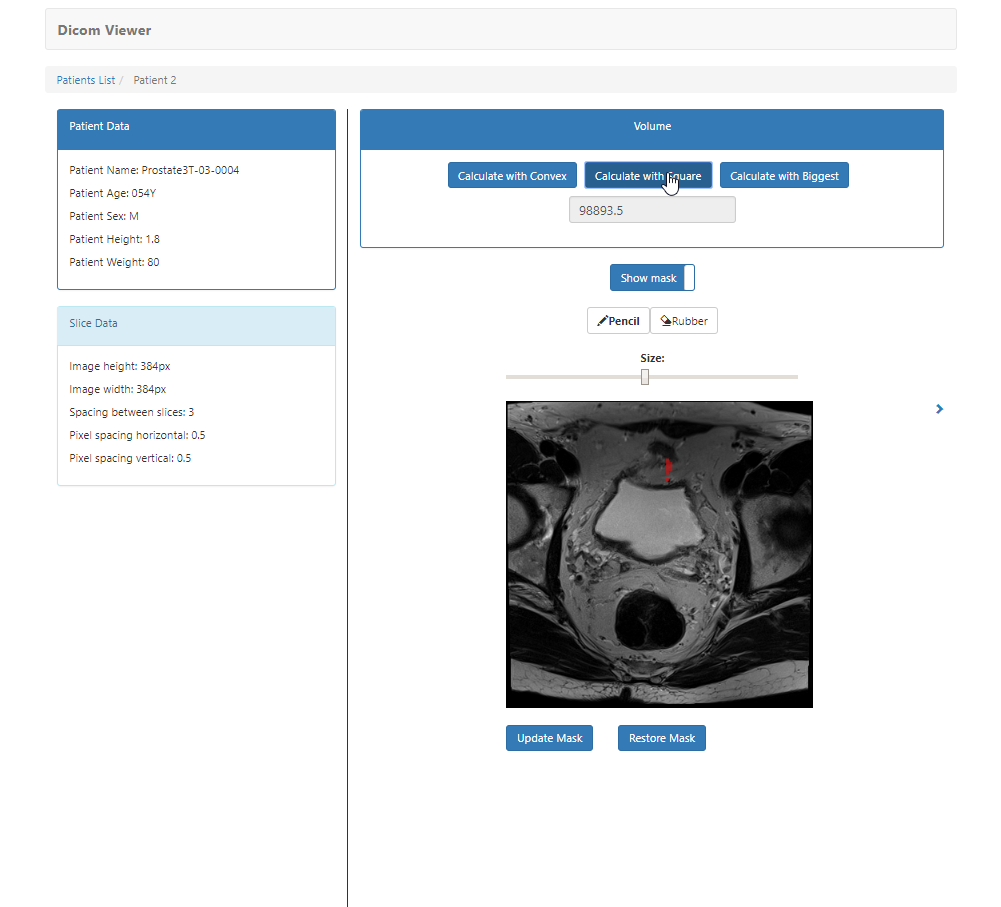
\includegraphics[width=0.5\textwidth]{FrontScreen/Patient/343.png}
	\captionof{figure}{Kalkulacja objęctości}
\end{minipage}

Aby przełączać się pomiędzy poszczególnymi warstwami należy nacisnąć przycisk po prawej lub lewej stronie obrazu.

\begin{minipage}{\linewidth}
	\centering
	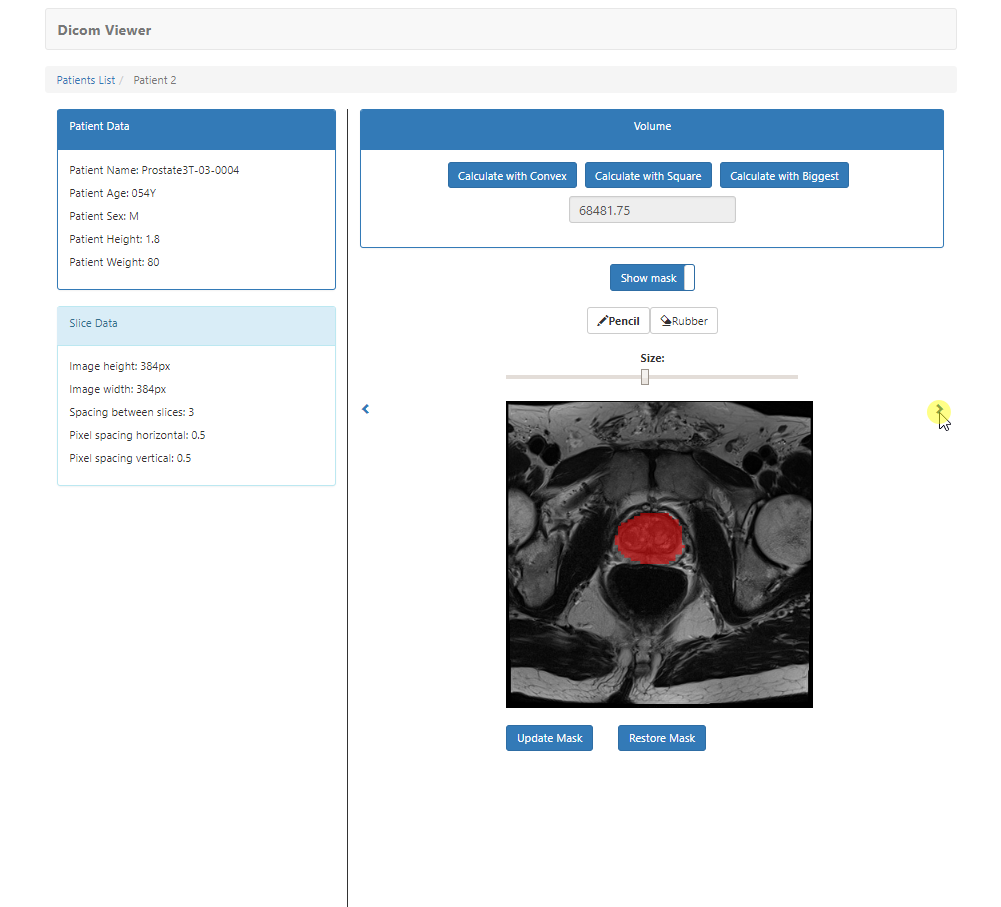
\includegraphics[width=0.5\textwidth]{FrontScreen/Editing/15.png}
	\captionof{figure}{Przechodzenie pomiędzy kolejnymi obrazami}
\end{minipage}

\subsection{Edycja obrazu}

Zapewniamy możliwość edycji masek obliczonych w procesie segmentacji. Udostępniamy opcje rysowani \textit{Pencil} oraz usuwania \textit{Rubber}. Po wybraniu narzędzia użytkownik może rysować po obrazie.

\begin{minipage}{\linewidth}
	\centering
	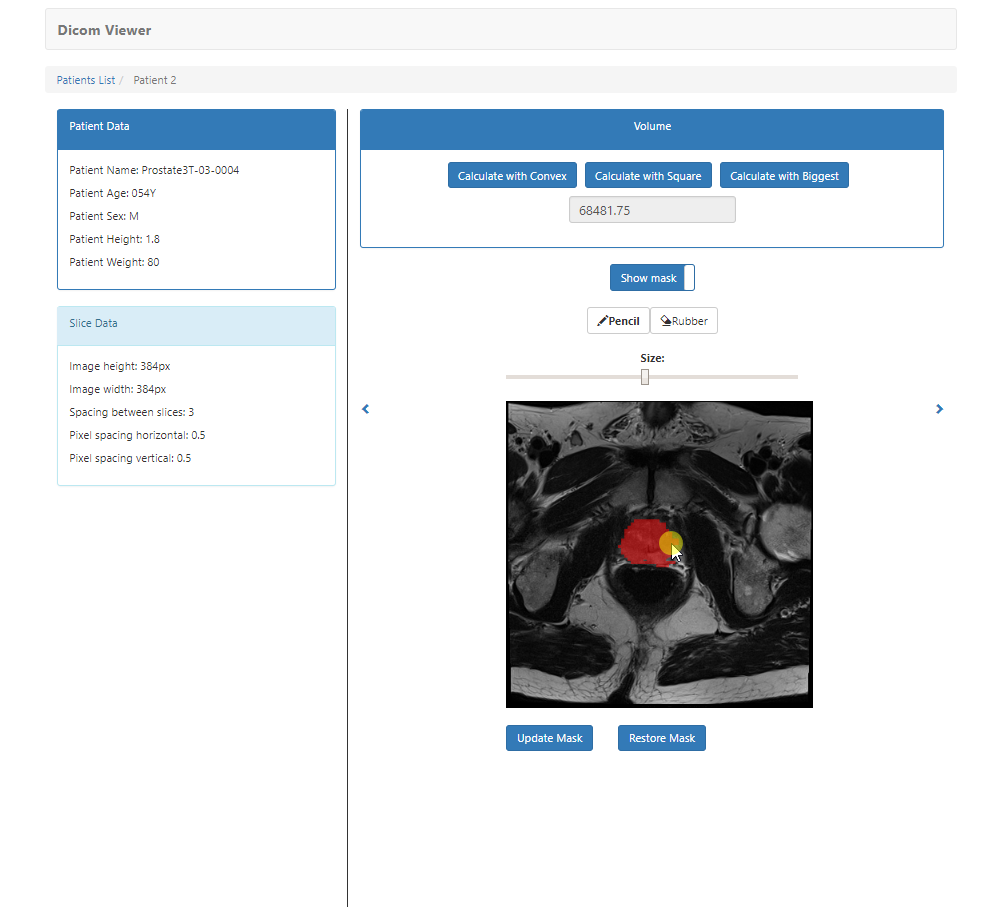
\includegraphics[width=0.5\textwidth]{FrontScreen/Editing/117.png}
	\captionof{figure}{Rysowanie maski}
\end{minipage}
\begin{minipage}{\linewidth}
	\centering
	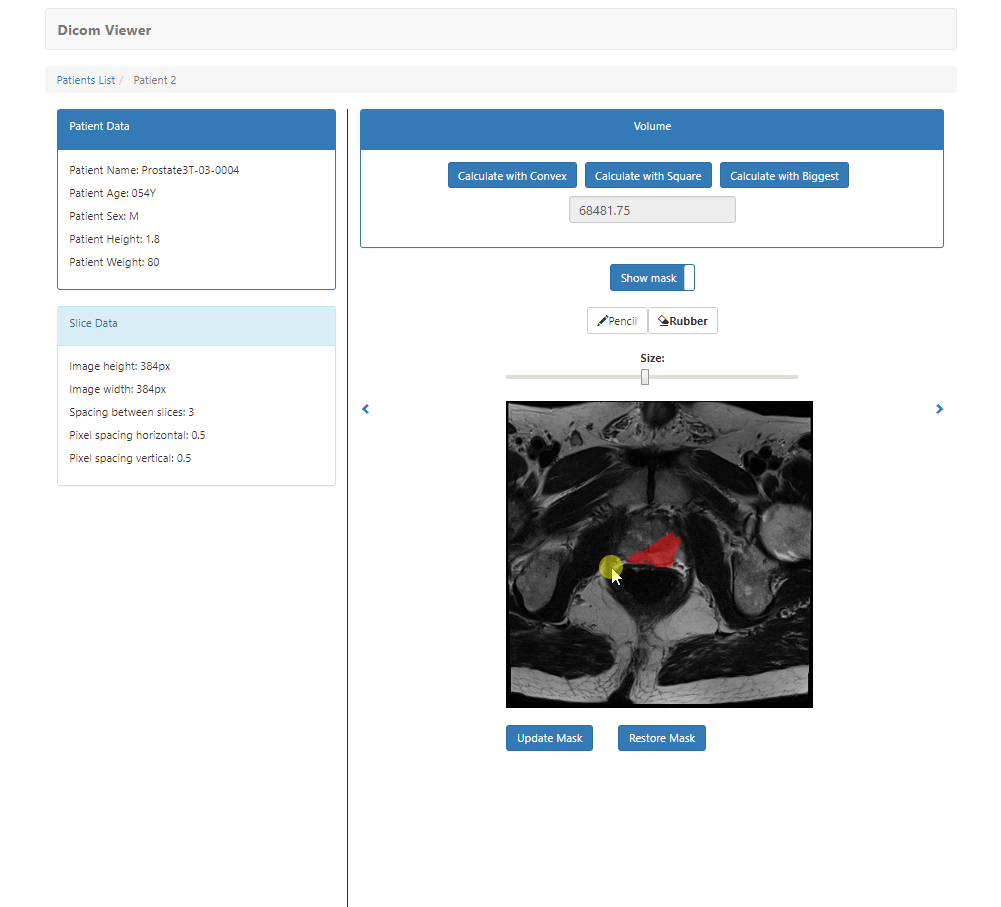
\includegraphics[width=0.5\textwidth]{FrontScreen/Editing/236.png}
	\captionof{figure}{Usuwanie maski}
\end{minipage}

Po zakończeniu edycji należy nacisnąć przycisk \textit{Update mask}.

\begin{minipage}{\linewidth}
	\centering
	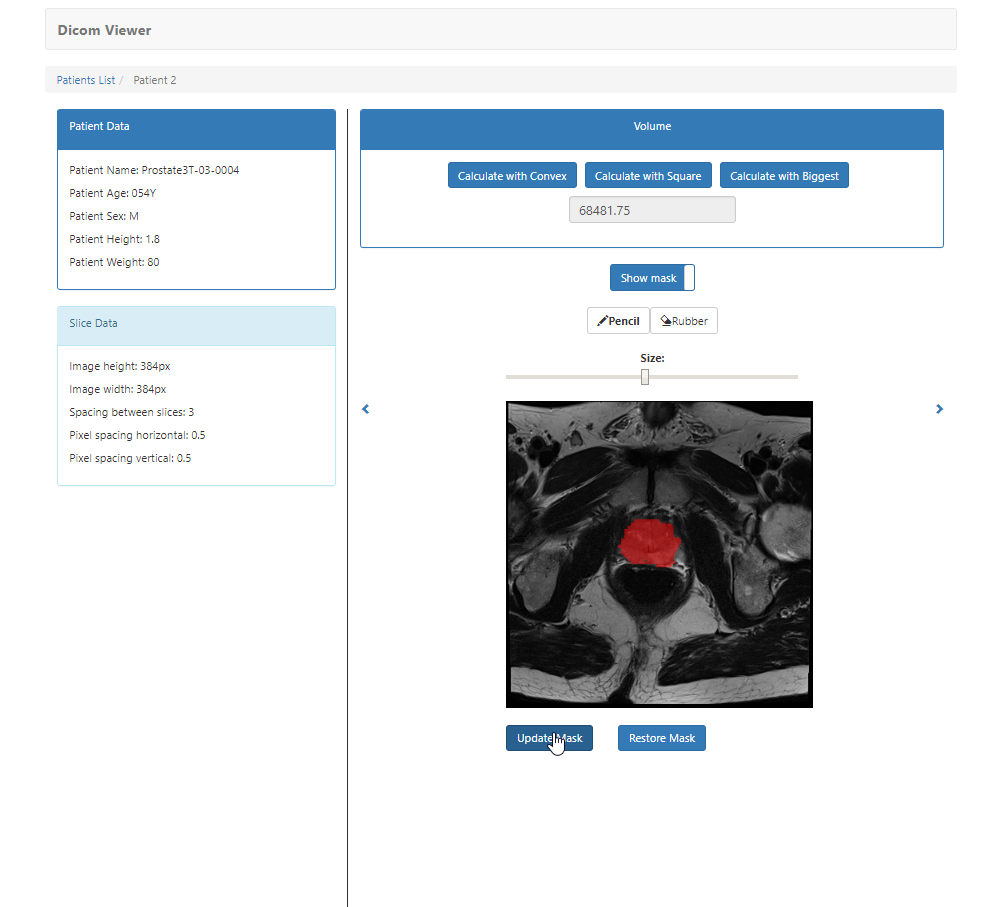
\includegraphics[width=0.5\textwidth]{FrontScreen/Editing/170.png}
	\captionof{figure}{Aktualizacja mask}
\end{minipage}

W przypadku gdy chcemy przywrócić pierwotną maskę znalezioną przez nasz algorytm segmentacji należy wybrać opcję \textit{Restore mask}

\begin{minipage}{\linewidth}
	\centering
	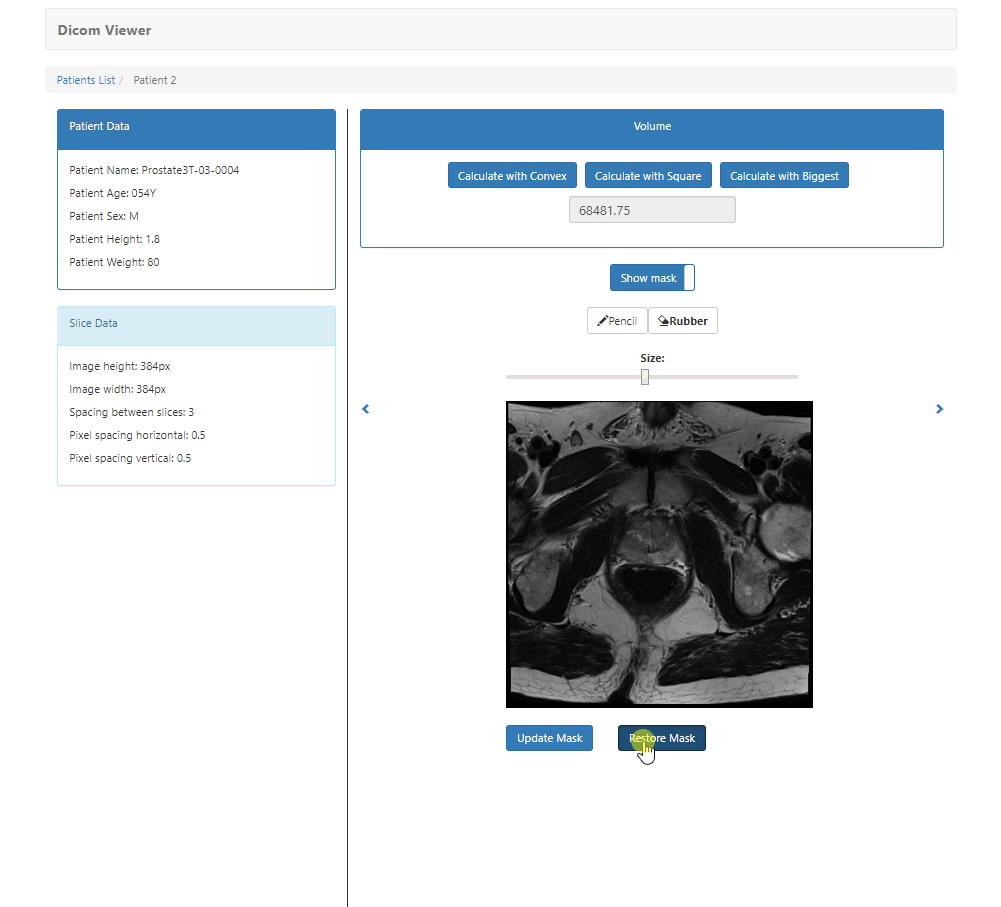
\includegraphics[width=0.5\textwidth]{FrontScreen/Editing/323.png}
	\captionof{figure}{Resetowanie maski}
\end{minipage}

Dodatkowo zapewniamy możliwość ukrycia maski w przypadku aby lekarz mógł przeglądać oryginał zdjęcia bez przysłaniania go maską.

\begin{minipage}{\linewidth}
	\centering
	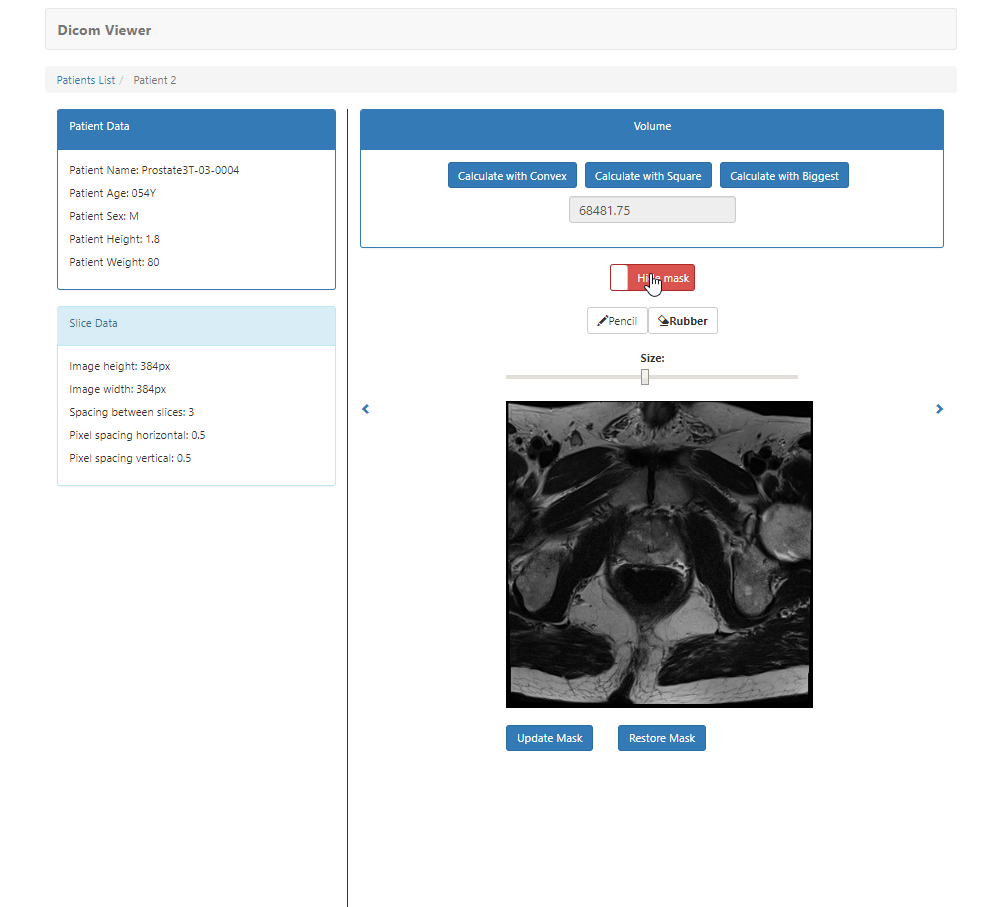
\includegraphics[width=0.5\textwidth]{FrontScreen/Editing/366.png}
	\captionof{figure}{Ukryj maskę}
\end{minipage}

\subsection{Integracja z systemem PACS}

Przycisk Import patient from PACS pozwala na pobranie danych o pacjencie z systemu PACS.

\begin{minipage}{\linewidth}
	\centering
	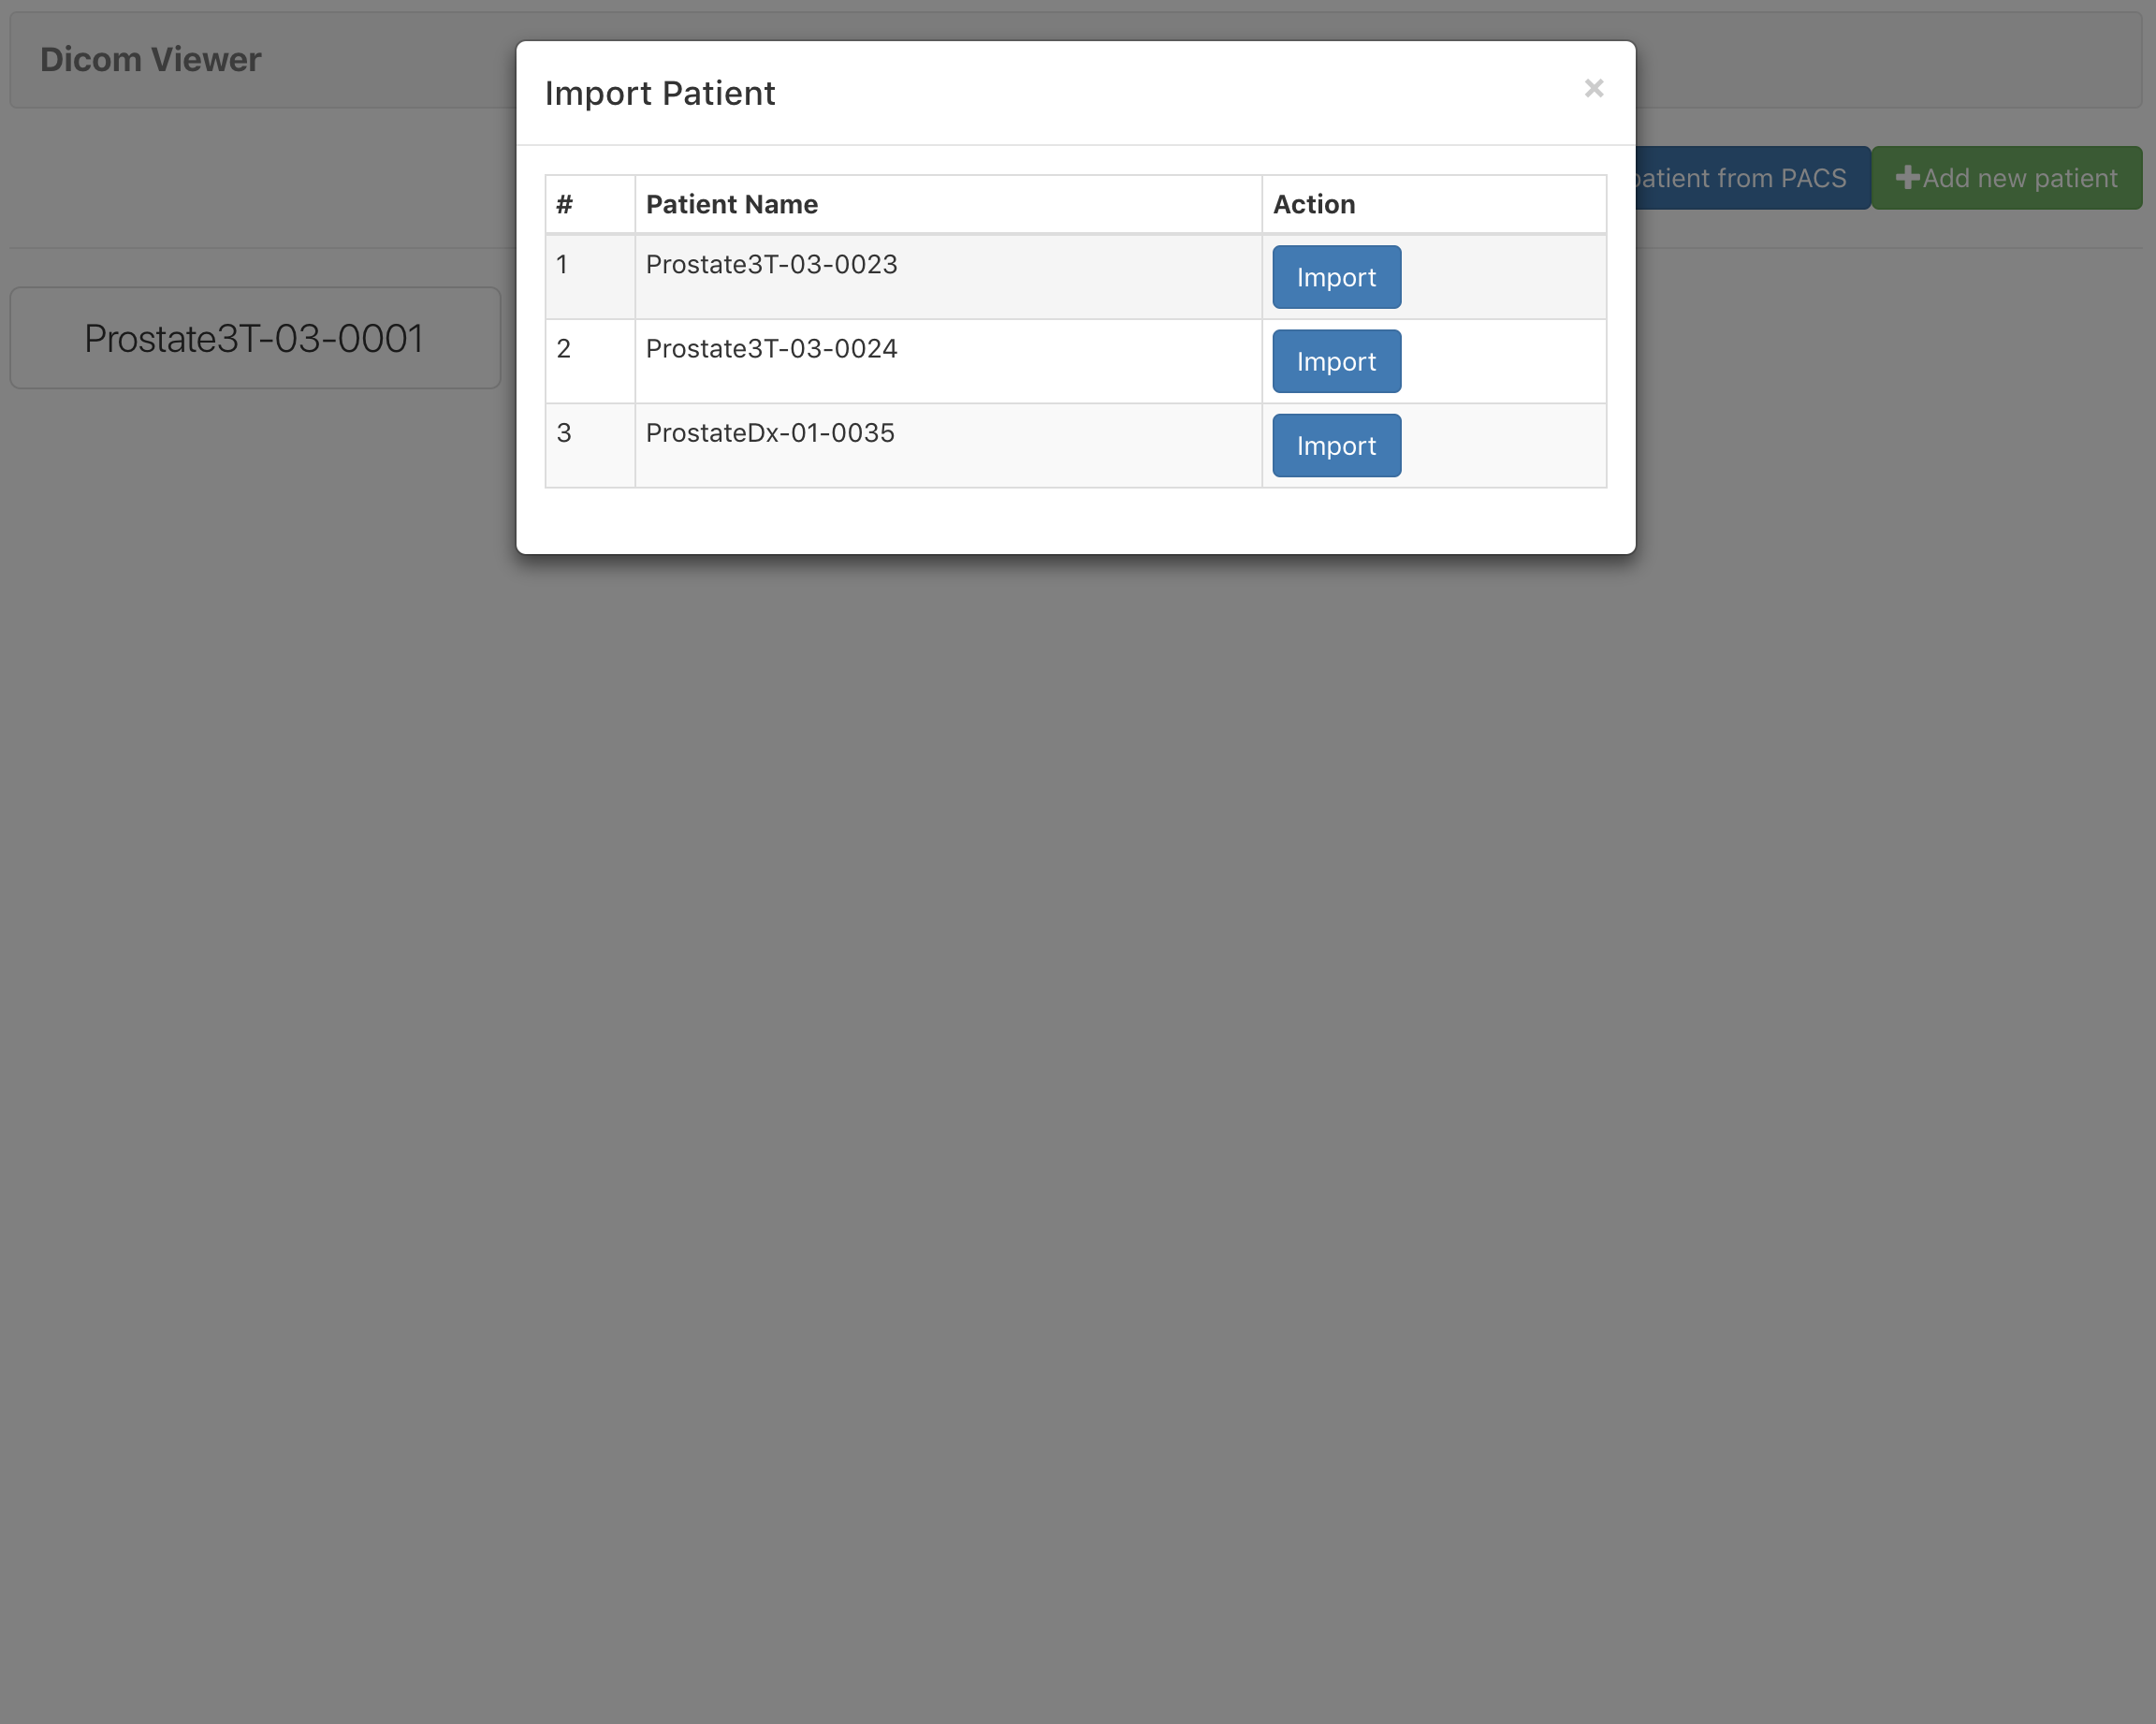
\includegraphics[width=0.5\textwidth]{FrontScreen/PACS/pacs.png}
	\captionof{figure}{Import z systemu PACS}
\end{minipage}

Połączenie z systemem jest konfigurowalne w plikach konifuracyjnych aplikacji fronowej. Import polega na pobraniu zanonimizowanych danych z serwera PACS i załadowaniu ich do naszej bazy danych.



% -------------------- Podsumowanie rezultatów -----------------------
\chapter{Podsumowanie rezultatów}
Rozdział jest poświęcony przedstawieniu rezultatów pracy nad omawianym systemem. Omówione zostaną testy, które zostały przeprowadzone w celu zbadania, czy stworzone rozwiązanie odpowiada założeniom, przedstawionym w rozdziale \textit{Specyfikacja}. 
\par
Głównym założeniem stworzenia aplikacji było wspieranie pracy lekarza poprzez zapewnienie systemu, który zapewniałby informację o predycji objętości prostaty z obrazów DICOM. Informacja o wielkości gruczołu ma dać lekarzowi szybką informację o potencjalnym wystąpieniu nowotworu prostaty. Cele został osiągnięty poprzez zaprojektowanie aplikacji, która daje możliwość przeglądania, segmentacji oraz liczenia objętości prostaty z różnych źródeł jakimi są pliki płaskie oraz szpitalny system PACS. Dodatkowo zapewniliśmy możliwość poprawy wyliczenia objętości poprzez ręczną możliwość edycji segmentacji. 

\section{Integracja z systemem informatycznym}
Podstawowym wymaganiem dotyczącym naszej pracy jest możliwość integracji i używania go razem z obecnymi w szpitalu systemami. Podczas naszej współpracy ze szpitalem niestety doszliśmy do wniosku, że nie jest możliwa integracja z systemem używanym na co dzień w szpitalu. System ten jest napisany przez firmę Philips i nie ma w nim możliwości instalacji wtyczek, a cały kod źródłowy jest utajniony. Przez co w naszym systemie proponujemy obejście tego problemu poprzez łączenie się z siecią szpitalna przez przeglądarkę i w ten sposób pobieranie danych. Rozwiązanie umożliwiające łatwą integrację z infrastrukturą szpitalną bez rozszerzania funkcjonalności przeglądarek DICOM. Alternatywnie można podłączyć serwer do szpitalnego systemu PACS przy użyciu sieci VPN. 
Rozwiązanie przy użyciu klienta po stronie przeglądarki ma kilka zalet, takich jak na przykład redukcje kosztów po stronie obsługi IT i umożliwia wprowadzanie zmian po stronie klienta bez konieczności manualnej instalacji oprogramowania. Co ma istotne znaczenie w używanych systemach szpitalnych.
\par
Aplikacja powstała przy wykorzystaniu najnowszych dostępnych technologii stąd w środowisku produkcyjnym (w szczególności w systemie szpitalnym) mogą pojawiać się problemy, wynikające z różnic pomiędzy naszym środowiskiem deweloperskim a szpitalną infrastrukturą IT. Wszystkie biblioteki jakich użyliśmy w pracy są stale rozwijane i zapewniają dobre wsparcie dla deweloperów. 
 
\section{Trudności}
W trakcie realizacji projektu napotkaliśmy kilka trudności. Największymi z nich były:
\begin{enumerate}
\item Problemy z integracją z siecią szpitalną. Wniosek jaki powstał po etapie analizy biznesowej, to, że uzyskanie odpowiednich uprawnień oraz dostępów do celu realizacji projektu jest niemożliwe. Stąd w naszej pracy integrację wykonaliśmy z lokalną instancją bazy PACS. Może to wprowadzać problemy przy realnej próbie integracji z systemem szpitalnym, gdyby okazało się, że systemy różnią się między sobą metodami dostępu w szczególności metodami udostępnianymi przez REST API.
\item  Największym problemem związanym z Pozyskanie danych szpitalnych był fakt, iż każdy system używa innego formatowania dokumentów, więc często występowały trudności z odczytaniem istotnych w naszym badaniu informacji.
\item Dane testowe jaki użyliśmy do uczenia sieci pochodzą z konkursu i zbiór testowy jest bardzo ograniczony. Może to powodować problemy z działaniem na realnych danych szpitalnych. 
\item Nie byliśmy w stanie sprawdzić dokładności algorytmu segmentacji z danymi realnych pacjentów szpitala, z uwagi na brak dostępu do danych. W analizie wyników brakowało nam najdokładniejszej informacji jaką jest objętość prostaty po zabiegu prostatektomii. Stąd nie jesteśmy w stanie zweryfikować wyników względem faktycznych wartości.
\end{enumerate}
Trudności spowodowały rozwiązanie problemów w alternatywne sposoby niż początkowo zakładaliśmy. Jednak  aby dopuścić rozwiązanie do użytku produkcyjnego powinny być rozwiązane. 

\section{Wnioski}
W trakcie realizacji pracy pojawiły się problemy, które zmusiły nas do zmiany początkowego podejścia. Finalna wersja spełnia wszystkie założenia przyjęte na początku projektu. Przedstawiony system może poprawić komfort pracy lekarza radiologa oraz zapewnić istotne informacje przy wystawianiu diagnozy pacjenta poprzez informację o przybliżonej wartości objętości gruczołu prostaty. Z uwagi na dużą złożoność systemu jest wiele możliwości wprowadzania usprawnień.

% -------------------- 6. Bibliografia -----------------------
% Bibliografia leksykograficznie wg nazwisk autorów

\begin{thebibliography}{20}%jak ktoś ma więcej książek, to niech wpisze większą liczbę

% \bibitem[numerek]{referencja} Autor, \emph{Tytuł}, Wydawnictwo, rok, strony
% cytowanie: \cite{referencja1, referencja 2,...}
\bibitem[1] {rynekZdrowia} \emph{Strona internetowa Rynek Zdrowia}, http://www.rynekzdrowia.pl/Serwis-Onkologia/Eksperci-wzrasta-zachorowalnosc-i-umieralnosc-Polakow-na-raka-prostaty,153015,1013.html
\bibitem[2] {konkurs} \emph{Dane konkursowe}, https://wiki.cancerimagingarchive.net/plugins/servlet/contentId=23691656/\#content/view/23691656
\bibitem[3] {standardDICOM} \emph {Standard DCIOM}, https://www.dicomstandard.org/
\bibitem[4] {OpenCV} \emph {Open CV} https://opencv.org/
\bibitem[5] {imageOrg} \emph {Przetwarzanie danych w medycynie} http://www.image-net.org/
\bibitem[6] {konkretny} \emph {Dane do uczenia sieci }https://wiki.cancerimagingarchive.net/display/Public/NCI-ISBI+2013+Challenge+-+Automated+Segmentation+of+Prostate+Structures
\bibitem[7] {zgłodzenie} \emph{Zgłoszenie do konkursu}, https://github.com/mirzaevinom/prostate\_segmentation
\bibitem[8]{Orthanc} \emph{Serwer PACS} https://www.orthanc-server.com/
\bibitem[9]{Philips} \emph{Aplikacje dostarczane przez firmę Philips} https://www.philips.com.eg/healthcare/resources/support-documentation/dicom-clinical-applications
\bibitem[10]{FP} \emph{Future Processing} https://www.future-processing.com/software-solutions/healthcare/
%\bibitem[2] https://www.nhs.uk/conditions/prostate-cancer/diagnosis/
%\bibitem[3] https://www.cancer.org/cancer/prostate-cancer/detection-diagnosis-staging/how-diagnosed.html
%\bibitem[5] https://lmb.informatik.uni-freiburg.de/people/ronneber/u-net/
\end{thebibliography}
\thispagestyle{empty}


% --- 7. Wykaz symboli i skrótów - jeśli nie ma, zakomentować
\chapter*{Wykaz symboli i skrótów}

\begin{tabular}{cl}
HTTP & Hypertext Transfer Protocol \\
IDE & Integrated Development Environment \\
np. & Na przykład \\
tzw. & Tak zwany \\
\end{tabular}
\thispagestyle{empty}


% ----- 8. Spis rysunków - jeśli nie ma, zakomentować --------
\listoffigures
\thispagestyle{empty}


% ------------ 9. Spis tabel - jak wyżej ------------------
\renewcommand{\listtablename}{Spis tabel}
\listoftables
\thispagestyle{empty}



% 10. Spis załączników - jak nie ma załączników, to zakomentować lub usunąć

\chapter*{Spis załączników}
\begin{enumerate}[itemsep = 0pt]
\item Załącznik 1 - Opis API
\end{enumerate}
\thispagestyle{empty}

% --------------------- 11. Załączniki ---------------------
% to jest po to, żeby było wiadomo, że załączniki znajdują się na końcu pracy

\newpage
\pagestyle{empty} 
\section{Załącznik 1 - Opis API}
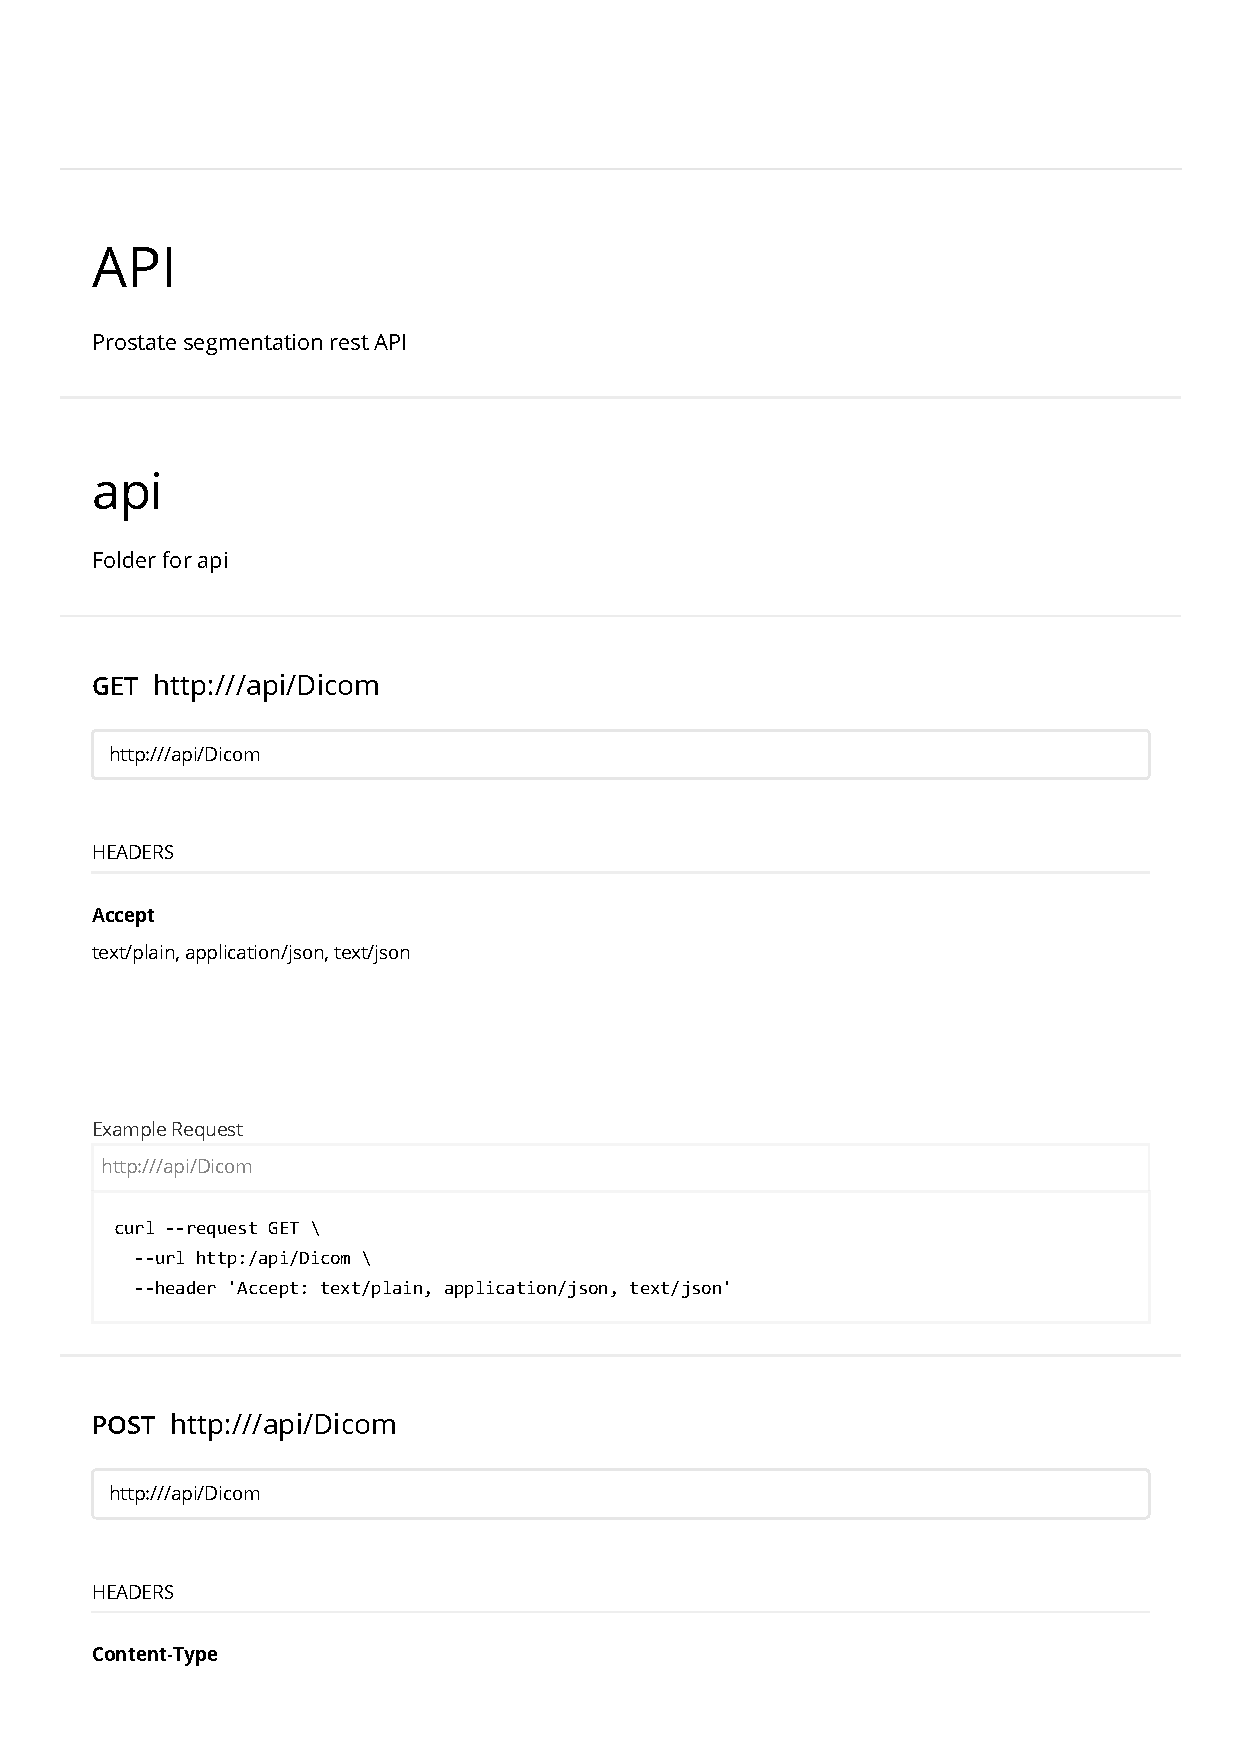
\includepdf[pages=-]{API.pdf}

\end{document}
